\documentclass[../main/main]{subfiles}

\setcounter{chapter}{5}
%\setcounter{page}{1}
\begin{document}
\chapter{適応的離散化手法の性能評価}
本章では,前章「設計変数の適応的離散化手法手法」で提案した二つの適応的離散化手法の性能をNSGA-IIと24個のベンチマーク問題を用いた評価する.

\section{実験条件}
\subsection{性能評価に使用するベンチマーク問題}
本実験では,影響評価で用いた19個のベンチマーク問題に加え,適応的離散化手法が意図したメカニズムとなっているかを確認するため,5つのベンチマーク問題を追加した24個のベンチマーク問題を用いた.
本実験で用いたベンチマーク問題を\Tabref{benchmark}に示す.

\begin{table}[htbp]
\fontsize{9.5pt}{9.5pt} \selectfont
\tabcolsep = 1pt
\centering
\caption{性能評価で用いるベンチマーク問題}
\vspace{0.1cm}
\label{benchmark}
\begin{tabular}{cccc||cccc}
\hline 
Problem & Obj. &Var. & Con. & Separability & Modality & Bias & Geometry \\
\hline 
DTLZ2 & M & N & - & separable & uni & - & concave\\
DTLZ3 & M & N & - & separable & multi & - & concave\\
DTLZ4 & M & N & - & separable & uni & \checkmark & concave\\
DTLZ7 & M & N & - & separable & uni & - & concave, disconnected\\
WFG2 & M & N & - & non-separable & multi & - & convex, disconnected\\
WFG4 & M & N & - & separable & multi & - & concave\\
WFG6 & M & N & - & non-separable & uni & - & concave\\
WFG7 & M & N & - & separable & uni & \checkmark & concave\\
WFG8 & M & N & - & non-separable & multi & - & concave\\
UF2 & 2 & N & - & non-separable & multi & - & convex\\
UF9& 3 & N & - & non-separable & multi & - & linear, disconnected\\
CF2 & 2 & N & 1 & non-separable & multi & - & convex, disconnected\\
CF7 & 2 & N & 2 & non-separable & multi & - & convex\\
C1DTLZ3 & M & N & 1 & separable & multi & - & concave\\
C2DTLZ2convex & M & N & 1 & separable & uni & - & convex, disconnected\\
C3DTLZ1 & M & N & M & separable & multi & - & convex(feasible surface is PF)\\
Car Side Impact & 3 & 7 & 10 & & & uncertain &\\
Welded Beam Design& 2 & 4 & 4 & & & uncertain &\\
Modified DTLZ2 & M & N & - & separable & uni & - & concave\\
Modified DTLZ3 & M & N & - & separable & multi & - & concave\\
Modified DTLZ4 & M & N & - & separable & uni & \checkmark & concave\\
Multi DTLZ2 & M & N & - & separable & uni & - & concave\\
Multi DTLZ3 & M & N & - & separable & multi & - & concave\\
Multi DTLZ4 & M & N & - & separable & uni & \checkmark  & concave\\
\hline
\end{tabular}
\\
{\scriptsize Obj. is the number of objectives; Var. is the number of variables; Con. is the number of constraints.}\\
{\scriptsize $M$ is the user predefined number of objectives; $N$ is the user predefined number of variables.}\\
{\scriptsize - indicates no value or no characteristic; \checkmark indicates that the problem has the characteristic.}\\
{\scriptsize The Car Side Impact and Welded Beam Design problems have uncertain characterisics because of engineering problems.}
\end{table}

表の見方は第4章「設計変数の離散化による影響評価」の表4.1.1と同様である.
本実験で追加した5つのベンチマーク問題の構造について次節以降で述べる.

\subsubsection{DTLZ7}
DTLZ7は  \Eqref{dtlz7}  で表される多目的問題である.
DTLZ7は,局所解を持たない単峰性の最適化問題であり,$M$目的の最適化問題として定式化した場合,$2^{M-1}$個の非連続な最適解部分を持つ問題である.
DTLZ2-4と同様に,設計変数$x_1,\cdots,x_{M-1}$は位置変数,設計変数$x_M,\cdots,x_n$は距離変数となるが,DTLZ2-4と異なり,距離変数$x_M$の最適値は$0$である.
したがって,DTLZ7の真のパレート最適解を得るためには,位置変数$x_1,\cdots,x_{M-1}$が一様に広がっており,すべての距離変数$x_M,\cdots,x_n$が$0$となる必要がある.

\begin{eqnarray} 
\left.
\begin{array}{ll}
Min. \quad f_{1}  (x_1) = x_1,\\
Min. \quad f_{2} (x_2) = x_2, \\
Min. \quad f_{3} (x_3) = x_3, \\
     \  \  \ $\vdots$    \qquad       \qquad \vdots \\
Min. \quad f_{M_1}(x_{M-1}) = x_{M-1},\\
Min. \quad f_{M} (\bm x) = (1 + g(\bm{x_M}))h(f_1,f_2,\cdots,f_{M-1},g),\\
with\ g(\bm{x}_{M}) = 1 + \cfrac{9}{|\bm{x_M}|} \sum_{x_i \in \bm{x_M}} x_i,  \\
\quad \quad \ h(f_1,f_2,\cdots,f_{M-1},g) = M - \sum^{M-1}_{i = 1}\left[ \cfrac{f_i}{1+g} (1 + sin(3\pi f_i))\right],\\
   \qquad    \  0 \le x_{i} \le 1,  for\ i = 1, 2, \ldots, n, \\
      \qquad    \        \bm x = (x_1,x_2, \ldots, x_n),\\
   \qquad    \        \bm{x}_M = (x_M,x_{M+1}, \ldots, x_n).
   \label{dtlz7} 
\end{array}
\right\}
\end{eqnarray}

\clearpage

\subsubsection{WFG8}
WFG8は第4章「設計変数の離散化による影響評価」の「4.1.1.2 WFG問題」で述べたように,形状関数とスケーリング関数によって設計変数は目的関数空間に射影される.
\Tabref{wfg8_comb}には,WFG8で用いる形状関数とスケーリング関数をまとめた.
形状関数とスケーリング関数については,それぞれ第4章「設計変数の離散化による影響評価」の表4.1.2,4.1.3を参照のこと.

\begin{table}[htbp]
\fontsize{10pt}{10pt} \selectfont
%\tabcolsep = 1pt
\centering
\caption{WFG8で用いる形状関数とスケーリング関数の組み合わせ}
\label{wfg8_comb}
\begin{tabular}{|c||c|l|}
\hline
Problem & Type & \multicolumn{1}{c|}{Setting}\\
\hline
All & Constants & $S_{m=1:M} = 2m$\\
&                       & $A_{1:M-1} = 1$ ( for WFG8)\\
\hline
All & Domains & $z_{i = 1:n,max} = 2i$\\
\hline
%WFG2 & Shape & $h_{m = 1:M-1} = convex_m$\\
%           &             & $h_M = disc_M ( with \alpha = \beta = 1 \ and \ A = 5)$\\
%           &     $t^1$   & $t^1_{i=1:k} = y_i$\\
%           &             &$ t^1_{i = k+1:n} = s\_linear(y_i, 0.35)$\\
%           &     $t^2$    & $t^2_{i = 1:k} = y_i$\\
%           &             & $t^2_{i = k+1:k+l/2} = r\_nonsep(\{ y_{k+2(i - k) - 1}, y_{k+2(i - k)} \},2)$\\
%           &     $t^3$    & $t^3_{i = 1:M-1} = r\_sum(\{ y_{(i-1)k / (M - 1) + 1}, \cdots, y_{ik / (M-1)} \}, \{1, \cdots, 1 \} )$\\
%           &              & $t^3_M = r\_sum(\{ y_{k+1}, \cdots, y_{k+l/2} \} , \{ 1, \cdots, 1\} )$\\
%\hline
%WFG4 & Shape &$ h_{m = 1:M} = concave_m$\\
%           &     $ t^1$  & $t^1_{i = 1:n} = s\_multi(y_i , 30, 10, 0.35)$\\
%           &  $t^2$      & $t^2_{i = 1:M-1} = r\_sum(\{ y_{(i-1)k / (M - 1) + 1}, \cdots, y_{ik / (M-1)} \}, \{1, \cdots, 1 \} )$\\
%           &                 & $t^2_M = r\_sum(\{ y_{k+1}, \cdots, y_n  \}, {1, \cdots, 1})$\\
%\hline
%WFG6 & Shape & $h_{m = 1:M} = concave_m$\\
%           &     $t^1$   & As $t^1$ from WFG2. (Linear shift.)\\
%           &     $t^2$    & $t^2_{i = 1:M-1} = r\_nonsep(\{ y_{(i - 1)k/(M-1)+1},\cdots, y_{ik/(M-1)} \}, k/(M-1))$\\
%           &             & $t^2_M = r\_nonsep(\{ y_{k+1},\cdots, y_{n} \},l)$\\
%\hline
%WFG7 & Shape & $h_{m = 1:M} = concave_m$\\
%           &     $ t^1$  & $t^1_{i = 1:k} = b\_param(y_i , r\_sum(\{ y_{i+1}, \cdots, y_n \}, \{1, \cdots, 1\}), \cfrac{0.98}{49.98},0.02,50)$\\
%           &                 & $ t^1_{i = k+1:n} = y_i$\\
%           &     $t^2$   & As $t^1$ from WFG2. (Linear shift.)\\
%           &     $t^3$   & As $t^2$ from WFG4. (Weighted sum reduction.)\\
%\hline  
WFG8 & Shape & $h_{m = 1:M} = concave_m$\\
           &     $ t^1$  & $t^1_{i = 1:k} = y_i$\\
           &                 & $t^1_{i = k+1:n} = b\_param(y_i , r\_sum(\{ y_{i+1}, \cdots, y_n \}, \{1, \cdots, 1\}), \cfrac{0.98}{49.98},0.02,50)$\\
           &     $t^2$   & As $t^1$ from WFG2. (Linear shift.)\\
           &     $t^3$   & As $t^2$ from WFG4. (Weighted sum reduction.)\\
\hline  
\end{tabular}
\end{table}

\subsubsection{Multi DTLZ問題}
Modified DTLZ問題をさらに改変したものである.
Modified DTLZ問題は距離変数の最適値が$0.1\pi$の1つだけである.
現実の設計問題を考えた場合,最適値が2つ以上存在する場合などが考えられるが,このような問題のベンチマーク問題は少ない.
そこで,Modified DTLZ問題を改変することで,最適値が2つとなる問題を提案する.
次節から,Multi DTLZ2,3,4について述べる.

\subsubsubsection{Multi DTLZ2,4}
Multi DTLZ2,4はそれぞれModified DTLZ2,4を改変したものである.
上述の\Eqref{gx_mod2}より,Modified DTLZ2,4は距離変数の最適値が$0.1\pi$の1点である.
Multi DTLZ2,4では\Eqref{gx_mod2}を\Eqref{gx_multi2}に改変することで距離変数の最適値が$0.1\pi$と$0.3\pi$の2点となる.

\begin{eqnarray}
g(\bm x_M) = 
\left\{
\begin{array}{rl}
\sum_{x_i \in \bm x_M} (x_i - 0.1 \pi)^2 & if  \ \ \  0 \leq x_i < 0.5\\
\sum_{x_i \in \bm x_M} (x_i - 0.3 \pi)^2 & otherwise \\
\end{array}
\right.
\label{gx_multi2}
\end{eqnarray}


\subsubsubsection{Multi DTLZ3}
Multi DTLZ3はModified DTLZ3を改変したものである.
上述の\Eqref{gx_mod3}より,Modified DTLZ3は距離変数の最適値が$0.1\pi$の1点である.
Multi DTLZ3では\Eqref{gx_mod3}を\Eqref{gx_multi3}に改変することで距離変数の最適値が$0.1\pi$と$0.3\pi$の2点となる.

\begin{eqnarray}
g(\bm x_M) = 
\left\{
\begin{array}{ll}
100[|\bm x_M| + \sum_{x_i \in \bm x_M} (x_i - 0.1\pi)^2 &\\
\qquad \qquad \qquad \qquad - cos(20 \pi (x_i - 0.1 \pi ))] & if  \  0 \leq x_i < 0.5 \\
100[|\bm x_M| + \sum_{x_i \in \bm x_M} (x_i - 0.3\pi)^2 &\\
\qquad \qquad \qquad \qquad - cos(20 \pi (x_i - 0.3 \pi ))] & otherwise \\
\end{array}
\right.
\label{gx_multi3}
\end{eqnarray}

\afterpage{\clearpage}



\subsection{計算条件}
本実験で用いるNSGA-IIの計算条件を \Tabref{tbl:condition} に示す.
また,各ベンチマーク問題の集団サイズ,世代数,目的関数の数,設計変数の数は,次節で説明する.
WFG問題におけるパラメータ$k$,$l$はそれぞれ$6$,$4$に設定した.
提案手法(SD,ePDF)の比較対象として,離散化の制御を行わず最適化を行ったもの(制御なし)を用いる.
SDを用いた提案手法の計算条件を\Tabref{tbl:sd_condition},ePDFを用いた提案手法の計算条件を\Tabref{tbl:pdf_condition}に示す.

\begin{table}[htbp]
\begin{minipage}{0.4\hsize}
\begin{center}
\caption{性能評価で用いるNSGA-IIの共通パラメータ}
\label{tbl:condition}
\begin{tabular}{c|c}
\hline 
parameter & value \\
\hline 
Crossover rate & 1.0\\
Mutation rate & 1/(\# of variables)\\
$\eta_c$ & 30 \\
$\eta_m$ & 20 \\
Trial & 10\\
\hline
\end{tabular}
\end{center}
\end{minipage}
\begin{minipage}{0.59\hsize}
\centering
\caption{SDで用いるパラメータ}
\label{tbl:sd_condition}
\begin{tabular}{c|c}
\hline 
parameter & value \\
\hline 
$d_{\rm min}$ & $2$\\
$d_{\rm max}$ & $8$\\
$\sigma_{\rm max}$ & $1 / \sqrt{12}$ \\
\hline
\end{tabular}
\\
{\footnotesize $1 / \sqrt{12}$ is standard deviation of uniform distribution.}
\end{minipage}
\end{table}

\begin{table}[htbp]
\centering
\caption{ePDFで用いるパラメータ}
\label{tbl:pdf_condition}
\begin{tabular}{c|c}
\hline 
parameter & value \\
\hline 
$d_{\rm min}$ & $2$\\
$d_{\rm max}$ & $8$\\
$h$ & $0.05$ \\
Kernel Function & Standard Normal Distribution\\
\hline
\end{tabular}
\\
{\footnotesize $h$ is bandwidth parameter in KDE.}
{\footnotesize Kernel Function is a function used by KDE.}
\end{table}




\section{数値実験の結果と考察}
非劣解の評価に関しては,今回はEngineering問題を除くベンチマーク問題では真のパレートフロントが既知であることと,収束性と多様性の観点から議論を行うため.多くの研究で利用されている Hyper Volume ではなく,解の収束性の指標である Generational Distance (GD) と解の収束性・多様性の総合指標である Inverted Generational Distance (IGD) を用いる.
また,各世代における実行可能な非劣解から算出されたGDとIGDの平均値を用いて評価する.
Engineering 問題においては,すべての結果の非劣解を合わせたものを擬似パレートフロントとし,同様にGDとIGDの平均値を求める.
さらに提案手法とその他の制御手法に有意な差があるかを調べるため,有意水準5\%でWilcoxonの順位和検定を行った.

%\section{GDの結果と考察}
\quad \Tabref{tbl:gd}は,各ベンチマーク問題において,SDを用いた提案手法(SD)とePDFを用いた提案手法(ePDF),離散化の制御を行わずに最適化を行った場合(制御なし)のGDの平均値の推移と各提案手法との検定結果を示している.
表中に示す Obj. は目的関数の数,Var. は設計変数の数,Gen は GD の平均値を求めた世代数を示している.
また,各世代において最小値となっている値は太字で示した.
さらに各提案手法と離散化の制御を行わなかったもの結果の間に有意差がある場合は$\checkmark$,有意差があると判断できない手法には$-$を記載した.

\Tabref{tbl:gd}を見ると,多くの問題でSDを用いた適応的離散化が最も小さいGD値となっていることが分かる.
また,ePDFを用いた適応的離散化においても制御なしと比較して多くの問題で小さい値となっている.
GDは値が小さいほど解の収束性が良いことを示す指標である.
したがって,設計変数を適応的に離散化するだけで収束性が向上する傾向があることが分かる.

統計検定の結果を見ると,SDを用いた適応的離散化は24個のベンチマーク問題のうち16個の問題で統計的に有意な差を持って優れたGDの推移となっていることが分かる.
また,統計的に有意な差を持って悪い推移となっている問題はWFG7とCF7の2つだけである.
ePDFを用いた適応的離散化においては,SDよりは少ないものの,9個の問題で統計的に優れた収束性が示されている.
さらに,ePDFでは統計的に有意な差を持って収束性が悪くなる問題は存在しなかった.
これらの結果からも,多くの問題において設計変数の適応的離散化は解の収束性を向上させる効果があることが確認された.
また,離散化をする際に用いる指標の違いにより,収束性に与える影響が異なることが分かった.

次に,問題ごとに細かく結果を見ていく.
まずDTLZ2-4,7の結果を見ると,どの問題でもSDを用いた適応的離散化が統計的に有意な差を持って最も良いGD値となっていることが分かる.
DTLZ問題は設計変数同士の相関関係がない点や,距離変数の最適値が$0.5$もしくは$0$であるため,粗く離散化した方が容易に最適値に収束しやすい問題だと考えられる.
したがって,適応的離散化により粗い離散化が行われたため,適応的離散化を用いた手法は離散化の制御を行わなかった場合に比べ,収束性が向上したことが考えられる.

WFG2,4,6,7,8の結果を見ると,DTLZ問題の結果とは異なり,最終世代のGD値の結果を見るとePDFを用いた適応的離散化が5つのうち3つの問題で最も良い結果となっている.
また,離散化の制御を行わなかったものも最終世代のGD値で比較すると2つの問題で最も良い結果となっている.
WFG問題はスケーリング関数により何度も設計変数が別空間に射影されるため,非線形性が非常に強い問題である.
また問題によっては設計変数同士に相関関係をあるため,進化の過程で設計変数空間に複数個密な分布が発生することが考えられる.
ePDFは設計変数空間が複雑な分布となっていてもその特徴を捉えやすく,適切な離散化が行えたことにより,最終的なGD値が良い値になったことが考えられる.
一方で,SDでは設計変数空間が複雑な分布となった場合,ePDFに比べ特徴を捉えづらく,適切な離散化ができなかったため,最終的なGD値が悪化してしまったことが考えられる.
統計検定の結果を見ると,WFG2では適応的離散化を用いた場合有意差を持って収束性が向上することが分かった.
また,WFG7では,有意差を持ってSDの結果が悪くなることが分かった.



\begin{table*}[htbp]
\fontsize{7.5pt}{7.5pt} \selectfont
\tabcolsep = 3pt
%\tabcolsep = 3pt
\centering
\caption{各適応的離散化手法を用いた場合と用いない場合のGDの平均値の推移}
\vspace{0.1cm}
\label{tbl:gd}
\begin{tabular}{c|ccccc||c|c|c|c|c}
\hline 
Problem & MG & PS & Obj. & Var. & Gen & \multicolumn{2}{c|}{SD} &\multicolumn{2}{c|}{ePDF} &制御なし\\ 
\hline
\multirow{3}{*}{DTLZ2}& & & & & 10 && $\bf 1.628  $ && $1.741  $ & $1.759  $\\ 
& 100&100&3&38&50& \checkmark &$\bf 1.671 \times 10^{-1}$ &-& $2.179 \times 10^{-1}$ & $2.565 \times 10^{-1}$\\ 
& & & & & 100&&$\bf 6.114 \times 10^{-2}$ && $9.541 \times 10^{-2}$ & $1.011 \times 10^{-1}$\\ 
\hline 
\multirow{3}{*}{DTLZ3}& & & & & 10 && $\bf 2.175 \times 10^{3}$ && $2.484 \times 10^{3}$ & $2.508 \times 10^{3}$\\ 
& 200&500&3&38&100& \checkmark &$\bf 1.508 \times 10^{2}$ &\checkmark& $2.792 \times 10^{2}$ & $4.039 \times 10^{2}$\\ 
& & & & & 200&&$\bf 2.661 \times 10$ && $4.349 \times 10$ & $6.669 \times 10$\\ 
\hline 
\multirow{3}{*}{DTLZ4}& & & & & 10 && $\bf 9.789 \times 10^{-1}$ && $1.292  $ & $1.223  $\\ 
& 100&300&3&38&50& \checkmark &$\bf 5.313 \times 10^{-2}$ &-& $8.692 \times 10^{-2}$ & $7.147 \times 10^{-2}$\\ 
& & & & & 100&&$\bf 2.060 \times 10^{-2}$ && $3.269 \times 10^{-2}$ & $2.522 \times 10^{-2}$\\ 
\hline 
\multirow{3}{*}{DTLZ7}& & & & & 10 && $\bf 7.060  $ && $8.295  $ & $8.145  $\\ 
& 100&100&3&38&50& \checkmark &$\bf 6.427 \times 10^{-1}$ &-& $1.276  $ & $1.306  $\\ 
& & & & & 100&&$\bf 1.491 \times 10^{-1}$ && $5.271 \times 10^{-1}$ & $5.442 \times 10^{-1}$\\ 
\hline 
\multirow{3}{*}{WFG2}& & & & & 10 && $2.350 \times 10^{-1}$ && $\bf 2.232 \times 10^{-1}$ & $2.428 \times 10^{-1}$\\ 
& 100&100&3&10&50& \checkmark &$\bf 5.586 \times 10^{-2}$ &\checkmark& $6.082 \times 10^{-2}$ & $7.141 \times 10^{-2}$\\ 
& & & & & 100&&$3.821 \times 10^{-2}$ && $\bf 3.748 \times 10^{-2}$ & $4.220 \times 10^{-2}$\\ 
\hline 
\multirow{3}{*}{WFG4}& & & & & 10 && $2.289 \times 10^{-1}$ && $2.139 \times 10^{-1}$ & $\bf 2.134 \times 10^{-1}$\\ 
& 100&100&3&10&50& - &$9.733 \times 10^{-2}$ &-& $\bf 9.001 \times 10^{-2}$ & $9.510 \times 10^{-2}$\\ 
& & & & & 100&&$6.698 \times 10^{-2}$ && $\bf 6.460 \times 10^{-2}$ & $6.654 \times 10^{-2}$\\ 
\hline 
\multirow{3}{*}{WFG6}& & & & & 10 && $4.868 \times 10^{-1}$ && $\bf 4.819 \times 10^{-1}$ & $4.900 \times 10^{-1}$\\ 
& 100&100&3&10&50& - &$\bf 2.171 \times 10^{-1}$ &-& $2.244 \times 10^{-1}$ & $2.268 \times 10^{-1}$\\ 
& & & & & 100&&$1.680 \times 10^{-1}$ && $1.797 \times 10^{-1}$ & $\bf 1.596 \times 10^{-1}$\\ 
\hline 
\multirow{3}{*}{WFG7}& & & & & 10 && $\bf 3.477 \times 10^{-1}$ && $3.575 \times 10^{-1}$ & $3.602 \times 10^{-1}$\\ 
& 100&100&3&10&50& \checkmark &$1.270 \times 10^{-1}$ &-& $1.144 \times 10^{-1}$ & $\bf 1.061 \times 10^{-1}$\\ 
& & & & & 100&&$8.698 \times 10^{-2}$ && $6.898 \times 10^{-2}$ & $\bf 6.517 \times 10^{-2}$\\ 
\hline 
\multirow{3}{*}{WFG8}& & & & & 10 && $7.337 \times 10^{-1}$ && $7.214 \times 10^{-1}$ & $\bf 7.015 \times 10^{-1}$\\ 
& 100&100&3&10&50& - &$2.934 \times 10^{-1}$ &-& $\bf 2.882 \times 10^{-1}$ & $2.939 \times 10^{-1}$\\ 
& & & & & 100&&$2.198 \times 10^{-1}$ && $\bf 1.977 \times 10^{-1}$ & $2.002 \times 10^{-1}$\\ 
\hline 
\multirow{3}{*}{UF2}& & & & & 10 && $3.405 \times 10^{-1}$ && $\bf 2.927 \times 10^{-1}$ & $3.001 \times 10^{-1}$\\ 
& 200&200&2&20&100& - &$2.661 \times 10^{-2}$ &\checkmark& $\bf 2.264 \times 10^{-2}$ & $2.64 \times 10^{-2}$\\ 
& & & & & 200&&$1.726 \times 10^{-2}$ && $\bf 1.400 \times 10^{-2}$ & $1.701 \times 10^{-2}$\\ 
\hline 
\multirow{3}{*}{UF9}& & & & & 10 && $\bf 2.752  $ && $2.810  $ & $2.771  $\\ 
& 200&300&3&20&100& - &$\bf 7.003 \times 10^{-1}$ &-& $7.153 \times 10^{-1}$ & $7.343 \times 10^{-1}$\\ 
& & & & & 200&&$\bf 5.068 \times 10^{-1}$ && $5.427 \times 10^{-1}$ & $5.320 \times 10^{-1}$\\ 
\hline 
\multirow{3}{*}{CF2}& & & & & 10 && $\bf 9.075 \times 10^{-1}$ && $9.586 \times 10^{-1}$ & $1.005  $\\ 
& 200&200&2&20&100& \checkmark &$\bf 1.506 \times 10^{-1}$ &\checkmark& $1.845 \times 10^{-1}$ & $2.302 \times 10^{-1}$\\ 
& & & & & 200&&$1.444 \times 10^{-1}$ && $\bf 1.113 \times 10^{-1}$ & $1.425 \times 10^{-1}$\\ 
\hline 
\multirow{3}{*}{CF7}& & & & & 10 && $\bf 2.628 \times 10$ && $2.686 \times 10$ & $2.706 \times 10$\\ 
& 200&200&2&20&100& \checkmark &$1.938  $ &-& $\bf 1.535  $ & $1.577  $\\ 
& & & & & 200&&$9.725 \times 10^{-1}$ && $\bf 5.473 \times 10^{-1}$ & $7.615 \times 10^{-1}$\\ 
\hline 
\multirow{3}{*}{C1DTLZ3}& & & & & 10 && $\bf 2.573 \times 10^{3}$ && $2.757 \times 10^{3}$ & $2.871 \times 10^{3}$\\ 
& 300&100&3&38&150& \checkmark &$\bf 1.361 \times 10^{2}$ &\checkmark& $2.214 \times 10^{2}$ & $3.267 \times 10^{2}$\\ 
& & & & & 300&&$\bf 7.301 \times 10$ && $9.030 \times 10$ & $1.243 \times 10^{2}$\\ 
\hline 
\multirow{3}{*}{C2DTLZ2 convex}& & & & & 10 && $\bf 3.948 \times 10$ && $5.962 \times 10$ & $7.017 \times 10$\\ 
& 300&100&3&38&150& \checkmark &$7.964 \times 10^{-2}$ &\checkmark& $\bf 7.492 \times 10^{-2}$ & $1.114 \times 10^{-1}$\\ 
& & & & & 300&&$5.569 \times 10^{-2}$ && $\bf 5.244 \times 10^{-2}$ & $9.449 \times 10^{-2}$\\ 
\hline 
\multirow{3}{*}{C3DTLZ1}& & & & & 10 && $\bf 1.140 \times 10^{3}$ && $1.168 \times 10^{3}$ & $1.152 \times 10^{3}$\\ 
& 300&100&3&38&150& \checkmark &$\bf 1.445 \times 10^{2}$ &\checkmark& $2.307 \times 10^{2}$ & $3.801 \times 10^{2}$\\ 
& & & & & 300&&$\bf 6.083 \times 10$ && $9.469 \times 10$ & $2.587 \times 10^{2}$\\ 
\hline 
\multirow{3}{*}{CarSideImpact}& & & & & 10 && $1.089 \times 10^{-1}$ && $\bf 1.008 \times 10^{-1}$ & $1.075 \times 10^{-1}$\\ 
& 100&300&3&7&50& - &$\bf 3.751 \times 10^{-2}$ &-& $3.765 \times 10^{-2}$ & $3.763 \times 10^{-2}$\\ 
& & & & & 100&&$\bf 3.109 \times 10^{-2}$ && $3.194 \times 10^{-2}$ & $3.167 \times 10^{-2}$\\ 
\hline 
\multirow{3}{*}{Welded Beam Design}& & & & & 10 && $\bf 2.762  $ && $2.954  $ & $8.898  $\\ 
& 100&300&2&4&50& \checkmark &$\bf 1.276 \times 10^{-2}$ &\checkmark& $1.884 \times 10^{-2}$ & $4.047 \times 10^{-2}$\\ 
& & & & & 100&&$4.390 \times 10^{-3}$ && $\bf 2.665 \times 10^{-3}$ & $8.827 \times 10^{-3}$\\ 
\hline 
\multirow{3}{*}{Modified DTLZ2}& & & & & 10 && $\bf 1.839  $ && $2.211  $ & $2.324  $\\ 
& 100&100&3&38&50& \checkmark &$\bf 1.641 \times 10^{-1}$ &-& $2.432 \times 10^{-1}$ & $2.827 \times 10^{-1}$\\ 
& & & & & 100&&$\bf 6.194 \times 10^{-2}$ && $1.030 \times 10^{-1}$ & $1.107 \times 10^{-1}$\\ 
\hline 
\multirow{3}{*}{Modified DTLZ3}& & & & & 10 && $\bf 2.226 \times 10^{3}$ && $2.636 \times 10^{3}$ & $2.628 \times 10^{3}$\\ 
& 200&500&3&38&100& \checkmark &$\bf 1.488 \times 10^{2}$ &-& $2.653 \times 10^{2}$ & $3.739 \times 10^{2}$\\ 
& & & & & 200&&$\bf 2.579 \times 10$ && $9.312 \times 10$ & $7.365 \times 10$\\ 
\hline 
\multirow{3}{*}{Modified DTLZ4}& & & & & 10 && $\bf 1.190  $ && $1.518  $ & $1.715  $\\ 
& 100&300&3&38&50& \checkmark &$\bf 5.539 \times 10^{-2}$ &-& $8.747 \times 10^{-2}$ & $1.000 \times 10^{-1}$\\ 
& & & & & 100&&$\bf 2.342 \times 10^{-2}$ && $3.050 \times 10^{-2}$ & $3.500 \times 10^{-2}$\\ 
\hline 
\multirow{3}{*}{Multi DTLZ2}& & & & & 10 && $\bf 6.995 \times 10^{-1}$ && $7.915 \times 10^{-1}$ & $7.791 \times 10^{-1}$\\ 
& 100&100&3&38&50& \checkmark &$\bf 8.519 \times 10^{-2}$ &-& $1.250 \times 10^{-1}$ & $1.163 \times 10^{-1}$\\ 
& & & & & 100&&$\bf 3.907 \times 10^{-2}$ && $5.691 \times 10^{-2}$ & $5.176 \times 10^{-2}$\\ 
\hline 
\multirow{3}{*}{Multi DTLZ3}& & & & & 10 && $\bf 2.017 \times 10^{3}$ && $2.333 \times 10^{3}$ & $2.394 \times 10^{3}$\\ 
& 200&500&3&38&100& \checkmark &$\bf 2.528 \times 10^{2}$ &\checkmark& $3.403 \times 10^{2}$ & $5.155 \times 10^{2}$\\ 
& & & & & 200&&$\bf 7.257 \times 10$ && $1.561 \times 10^{2}$ & $1.586 \times 10^{2}$\\ 
\hline 
\multirow{3}{*}{Multi DTLZ4}& & & & & 10 && $\bf 4.561 \times 10^{-1}$ && $5.459 \times 10^{-1}$ & $5.982 \times 10^{-1}$\\ 
& 100&300&3&38&50& \checkmark &$\bf 3.238 \times 10^{-2}$ &-& $5.687 \times 10^{-2}$ & $5.349 \times 10^{-2}$\\ 
& & & & & 100&&$\bf 1.934 \times 10^{-2}$ && $2.833 \times 10^{-2}$ & $2.690 \times 10^{-2}$\\ 
\hline 
\end{tabular}
%\\
%{\footnotesize MG is the number of generation set; PS is the number of population size set.}\\
%{\footnotesize Obj. is the number of objectives; Var. is the number of variables.}\\
%{\footnotesize Gen indicates the generation that results were computed on.} \\
%{\footnotesize $\checkmark$ indicates that there is significant difference between using each indicator and UD in each problem.}\\
%{\footnotesize - indicates that there is not significant difference between using each indicator and UD in each problem.}
\end{table*}

UF2,9,CF2,7の結果を見ると概ねどちらかの適応的離散化手法が良い結果となっている.
まずUF2については,ePDFの結果が統計的有意差を持って最も良くなっており,SDの結果と制御なしの結果の間には有意差が存在しなかった.
そのため,UF2では適切な離散化を施すことで収束性が向上する可能性があることが分かった.
ePDFは複雑な解の分布の特徴を捉えやすく,non-separableやmultiといった特徴を持つ問題に対しても適切に離散化できる可能性が高いことが考えられる.
UF9では,適応的離散化手法と離散化の制御なしの場合の間に有意差は存在しなかった.
しかし,各世代を通してSDが最も良いGD値となっており,離散化が収束性に影響している可能性が考えられる.
CF2では,適応的離散化手法が有意差を持ってGD値が良い推移を取っていることが分かる.
したがって,適切な離散化を施すことで収束性が向上することが分かった.
また最終的に,ePDFが最も小さいGD値となっており,このことからも複雑な問題に対しても適切に離散化できる可能性が高いことが分かる.
CF7では,ePDFが最も小さいGD値となっているものの,SDが有意差を持って高いGD値となっていることが分かる.
このことからも,ePDFはSDに比べ,複雑な問題に対しても効果的に離散化が行えることが分かった.

C1DTLZ3,C2DTLZ2 convex, C3DTLZ1の結果を見るとどの問題も適応的離散化を施すことで有意差を持って収束性が向上する結果となった.
CDTLZ問題は,基本的な問題構造はDTLZと同様だが制約条件がつく問題である.
このことから,制約条件がある場合でも,適応的離散化がうまく働き収束性が向上することが分かった.

Car Side Impact 問題,Welded Beam Design 問題では,Car Side Impact 問題では統計的有意差は見られなかったが,Welded Beam Design 問題ではいずれの適応的離散化手法も統計的有意差を持って良い結果となっている.
また,有意差は見られなかったものの Car Side Impact 問題ではSDが最終的に最も小さい値となっており,実際の設計問題を模擬した問題においても,適応的離散化が収束性を向上させる可能性があることが確認された.

Modified DTLZ2-4 の結果見ると,いずれの問題においてもSDの結果が統計的有意差を持って最も良い結果となっている.
対照的にePDFは離散化の制御を行わなかった場合と比較し,統計的有意差は見られなかった.
DTLZ問題は変数同士に相関関係を持たず,非常に単純な構造をしているため,SDの評価のみで十分に分布を評価することができる.
ePDFでは解の分布を精細に評価するために,誤差や外れ値に影響されやすく,単純な分布の際は反って誤った評価をしてしまう場合が考えられる.
したがって,適切に離散化が行えず,離散化を行わなかったものと同等の結果となってしまったものと考えられる.
この点は,ePDFの課題として挙げられる.

Multi DTLZ2-4では,いずれの問題においてもSDの結果が統計的有意差を持って最も良い結果となっている.
またePDFも Multi DTLZ3において,制御なしと比較し統計的に優れた収束性を持っていることが分かる.
Multi DTLZ問題においても上述のModified DTLZ問題と同様に非常に単純な構造をしているため,SDの評価のみで十分に分布を評価することができるため,SDが最も良い結果となったことが考えられる.
また,Multi DTLZ問題は,ある設計変数空間に2点最適解が存在する構造となっているため,複数密な分布が生成される場合があり,Multi DTLZ3において良い結果となったことが考えられる.

以上の結果から,適応的離散化は多くの問題で収束性を加速させることが分かった.
特にSDを用いた適応的離散化は24個のうち16の問題で統計的に優れた収束性があることが分かった.
また,問題の性質から,解の分布状態の評価指標としてSDを用いた方が良い場合とePDFを用いた方が良い場合があることが分かった.
特に,設計変数同士に相関関係があるなど,設計変数空間に複数密な分布が得られやすいような問題に対してはePDFの方が収束性向上に効果があることが分かった.

%\clearpage

%\section{IGDの結果と考察}
\quad \Tabref{tbl:igd}は,各ベンチマーク問題において,SDを用いた提案手法(SD)とePDFを用いた提案手法(ePDF),離散化の制御を行わずに最適化を行った場合(制御なし)のIGDの平均値の推移と各提案手法との検定結果を示している.
表中に示す Obj. は目的関数の数,Var. は設計変数の数,Gen は IGD の平均値を求めた世代数を示している.
また,各世代において最小値となっている値は太字で示した.
さらに各提案手法と離散化の制御を行わなかったもの結果の間に有意差がある場合は$\checkmark$,有意差があると判断できない手法には$-$を記載した.

IGD値は小さければ小さいほど収束性が良く多様性も良いという指標であり,収束性の指標であるGD値と比較することで解の多様性について議論することができる.
\Tabref{tbl:igd}を見ると,\Tabref{tbl:gd}のGDの結果と比較して,最小のIGD値となっている手法にばらつきがあることが分かる.
しかし,どの場合も概ね同程度のオーダーのIGD値が得られていることから,適応的離散化手法では収束性を高めながらもある程度多様性を維持することができており,設計の意図通りの効果が得られたことが分かる.
%また,\Tabref{tbl:gd}と比較し,離散化の制御を行わなかった場合が最小のIGD値となっている場合が多い
%このことから,適応的離散化手法は収束性を向上させる傾向はあるが,一概に解の多様性も向上させる傾向があるとは言えないと結果となった.



\begin{table*}[htbp]
\fontsize{7.5pt}{7.5pt} \selectfont
\tabcolsep = 3pt
%\tabcolsep = 3pt
\centering
\caption{各適応的離散化手法を用いた場合と用いない場合のIGDの平均値の推移}
\vspace{0.1cm}
\label{tbl:igd}
\begin{tabular}{c|ccccc||c|c|c|c|c}
\hline 
Problem & MG & PS & Obj. & Var. & Gen & \multicolumn{2}{c|}{SD} &\multicolumn{2}{c|}{ePDF} &制御なし\\ 
\hline
\multirow{3}{*}{DTLZ2}& & & & & 10 && $1.276  $ && $\bf 1.255  $ & $1.264  $\\ 
& 100&100&3&38&50& - &$\bf 1.497 \times 10^{-1}$ &-& $1.607 \times 10^{-1}$ & $1.782 \times 10^{-1}$\\ 
& & & & & 100&&$5.709 \times 10^{-2}$ && $\bf 5.549 \times 10^{-2}$ & $6.213 \times 10^{-2}$\\ 
\hline 
\multirow{3}{*}{DTLZ3}& & & & & 10 && $\bf 1.577 \times 10^{3}$ && $1.647 \times 10^{3}$ & $1.666 \times 10^{3}$\\ 
& 200&500&3&38&100& \checkmark &$\bf 1.181 \times 10^{2}$ &\checkmark& $1.659 \times 10^{2}$ & $2.195 \times 10^{2}$\\ 
& & & & & 200&&$\bf 2.270 \times 10$ && $3.245 \times 10$ & $4.607 \times 10$\\ 
\hline 
\multirow{3}{*}{DTLZ4}& & & & & 10 && $\bf 1.152  $ && $1.159  $ & $1.236  $\\ 
& 100&300&3&38&50& \checkmark &$2.351 \times 10^{-1}$ &\checkmark& $\bf 7.879 \times 10^{-2}$ & $3.517 \times 10^{-1}$\\ 
& & & & & 100&&$1.879 \times 10^{-1}$ && $\bf 3.076 \times 10^{-2}$ & $2.507 \times 10^{-1}$\\ 
\hline 
\multirow{3}{*}{DTLZ7}& & & & & 10 && $\bf 5.908  $ && $6.235  $ & $6.182  $\\ 
& 100&100&3&38&50& \checkmark &$\bf 5.914 \times 10^{-1}$ &-& $8.121 \times 10^{-1}$ & $8.245 \times 10^{-1}$\\ 
& & & & & 100&&$\bf 1.783 \times 10^{-1}$ && $3.283 \times 10^{-1}$ & $3.037 \times 10^{-1}$\\ 
\hline 
\multirow{3}{*}{WFG2}& & & & & 10 && $5.272 \times 10^{-1}$ && $5.133 \times 10^{-1}$ & $\bf 4.964 \times 10^{-1}$\\ 
& 100&100&3&10&50& \checkmark &$3.631 \times 10^{-1}$ &\checkmark& $3.412 \times 10^{-1}$ & $\bf 3.072 \times 10^{-1}$\\ 
& & & & & 100&&$3.428 \times 10^{-1}$ && $3.40 \times 10^{-1}$ & $\bf 2.713 \times 10^{-1}$\\ 
\hline 
\multirow{3}{*}{WFG4}& & & & & 10 && $\bf 4.360 \times 10^{-1}$ && $4.778 \times 10^{-1}$ & $4.638 \times 10^{-1}$\\ 
& 100&100&3&10&50& - &$\bf 1.293 \times 10^{-1}$ &-& $1.593 \times 10^{-1}$ & $1.439 \times 10^{-1}$\\ 
& & & & & 100&&$\bf 8.883 \times 10^{-2}$ && $1.031 \times 10^{-1}$ & $9.700 \times 10^{-2}$\\ 
\hline 
\multirow{3}{*}{WFG6}& & & & & 10 && $5.071 \times 10^{-1}$ && $\bf 4.927 \times 10^{-1}$ & $5.013 \times 10^{-1}$\\ 
& 100&100&3&10&50& - &$\bf 2.207 \times 10^{-1}$ &-& $2.255 \times 10^{-1}$ & $2.273 \times 10^{-1}$\\ 
& & & & & 100&&$1.679 \times 10^{-1}$ && $1.760 \times 10^{-1}$ & $\bf 1.591 \times 10^{-1}$\\ 
\hline 
\multirow{3}{*}{WFG7}& & & & & 10 && $5.242 \times 10^{-1}$ && $5.096 \times 10^{-1}$ & $\bf 4.986 \times 10^{-1}$\\ 
& 100&100&3&10&50& \checkmark &$2.500 \times 10^{-1}$ &-& $2.359 \times 10^{-1}$ & $\bf 2.345 \times 10^{-1}$\\ 
& & & & & 100&&$2.022 \times 10^{-1}$ && $1.815 \times 10^{-1}$ & $\bf 1.664 \times 10^{-1}$\\ 
\hline 
\multirow{3}{*}{WFG8}& & & & & 10 && $7.920 \times 10^{-1}$ && $7.807 \times 10^{-1}$ & $\bf 7.708 \times 10^{-1}$\\ 
& 100&100&3&10&50& - &$3.691 \times 10^{-1}$ &-& $\bf 3.618 \times 10^{-1}$ & $3.624 \times 10^{-1}$\\ 
& & & & & 100&&$2.882 \times 10^{-1}$ && $2.670 \times 10^{-1}$ & $\bf 2.622 \times 10^{-1}$\\ 
\hline 
\multirow{3}{*}{UF2}& & & & & 10 && $2.204 \times 10^{-1}$ && $\bf 2.117 \times 10^{-1}$ & $2.283 \times 10^{-1}$\\ 
& 200&200&2&20&100& \checkmark &$\bf 4.259 \times 10^{-2}$ &\checkmark& $4.702 \times 10^{-2}$ & $5.312 \times 10^{-2}$\\ 
& & & & & 200&&$\bf 3.524 \times 10^{-2}$ && $4.546 \times 10^{-2}$ & $4.534 \times 10^{-2}$\\ 
\hline 
\multirow{3}{*}{UF9}& & & & & 10 && $\bf 1.005  $ && $1.086  $ & $1.011  $\\ 
& 200&300&3&20&100& \checkmark &$2.864 \times 10^{-1}$ &\checkmark& $2.808 \times 10^{-1}$ & $\bf 2.508 \times 10^{-1}$\\ 
& & & & & 200&&$2.257 \times 10^{-1}$ && $2.146 \times 10^{-1}$ & $\bf 1.880 \times 10^{-1}$\\ 
\hline 
\multirow{3}{*}{CF2}& & & & & 10 && $5.045 \times 10^{-1}$ && $\bf 5.015 \times 10^{-1}$ & $5.257 \times 10^{-1}$\\ 
& 200&200&2&20&100& \checkmark &$1.089 \times 10^{-1}$ &\checkmark& $1.070 \times 10^{-1}$ & $\bf 1.063 \times 10^{-1}$\\ 
& & & & & 200&&$1.054 \times 10^{-1}$ && $1.017 \times 10^{-1}$ & $\bf 9.750 \times 10^{-2}$\\ 
\hline 
\multirow{3}{*}{CF7}& & & & & 10 && $\bf 1.760 \times 10$ && $1.785 \times 10$ & $1.851 \times 10$\\ 
& 200&200&2&20&100& \checkmark &$8.404 \times 10^{-1}$ &\checkmark& $5.173 \times 10^{-1}$ & $\bf 4.863 \times 10^{-1}$\\ 
& & & & & 200&&$4.401 \times 10^{-1}$ && $4.077 \times 10^{-1}$ & $\bf 3.775 \times 10^{-1}$\\ 
\hline 
\multirow{3}{*}{C1DTLZ3}& & & & & 10 && $1.953 \times 10^{3}$ && $1.967 \times 10^{3}$ & $\bf 1.950 \times 10^{3}$\\ 
& 300&100&3&38&150& \checkmark &$\bf 1.232 \times 10^{2}$ &\checkmark& $1.483 \times 10^{2}$ & $1.956 \times 10^{2}$\\ 
& & & & & 300&&$\bf 6.410 \times 10$ && $7.591 \times 10$ & $8.024 \times 10$\\ 
\hline 
\multirow{3}{*}{C2DTLZ2 convex}& & & & & 10 && $\bf 3.897  $ && $4.042  $ & $4.338  $\\ 
& 300&100&3&38&150& \checkmark &$7.372 \times 10^{-2}$ &\checkmark& $\bf 7.317 \times 10^{-2}$ & $7.828 \times 10^{-2}$\\ 
& & & & & 300&&$6.928 \times 10^{-2}$ && $\bf 6.84 \times 10^{-2}$ & $7.260 \times 10^{-2}$\\ 
\hline 
\multirow{3}{*}{C3DTLZ1}& & & & & 10 && $6.831 \times 10^{2}$ && $\bf 6.752 \times 10^{2}$ & $6.938 \times 10^{2}$\\ 
& 300&100&3&38&150& \checkmark &$\bf 6.346 \times 10$ &\checkmark& $8.339 \times 10$ & $8.776 \times 10$\\ 
& & & & & 300&&$\bf 2.551 \times 10$ && $2.630 \times 10$ & $3.508 \times 10$\\ 
\hline 
\multirow{3}{*}{CarSideImpact}& & & & & 10 && $\bf 3.348 \times 10^{-1}$ && $3.384 \times 10^{-1}$ & $3.652 \times 10^{-1}$\\ 
& 100&300&3&7&50& - &$\bf 5.361 \times 10^{-2}$ &-& $5.504 \times 10^{-2}$ & $5.674 \times 10^{-2}$\\ 
& & & & & 100&&$3.509 \times 10^{-2}$ && $3.522 \times 10^{-2}$ & $\bf 3.480 \times 10^{-2}$\\ 
\hline 
\multirow{3}{*}{Welded Beam Design}& & & & & 10 && $5.077 \times 10^{-1}$ && $5.136 \times 10^{-1}$ & $\bf 4.921 \times 10^{-1}$\\ 
& 100&300&2&4&50& \checkmark &$1.068 \times 10^{-1}$ &\checkmark& $8.372 \times 10^{-2}$ & $\bf 6.592 \times 10^{-2}$\\ 
& & & & & 100&&$9.295 \times 10^{-2}$ && $6.907 \times 10^{-2}$ & $\bf 4.521 \times 10^{-2}$\\ 
\hline 
\multirow{3}{*}{Modified DTLZ2}& & & & & 10 && $\bf 1.405  $ && $1.456  $ & $1.501  $\\ 
& 100&100&3&38&50& - &$\bf 1.507 \times 10^{-1}$ &-& $1.797 \times 10^{-1}$ & $1.944 \times 10^{-1}$\\ 
& & & & & 100&&$\bf 6.230 \times 10^{-2}$ && $6.332 \times 10^{-2}$ & $6.526 \times 10^{-2}$\\ 
\hline 
\multirow{3}{*}{Modified DTLZ3}& & & & & 10 && $1.683 \times 10^{3}$ && $\bf 1.67 \times 10^{3}$ & $1.757 \times 10^{3}$\\ 
& 200&500&3&38&100& \checkmark &$\bf 1.133 \times 10^{2}$ &-& $1.943 \times 10^{2}$ & $2.152 \times 10^{2}$\\ 
& & & & & 200&&$\bf 2.249 \times 10$ && $7.016 \times 10$ & $4.999 \times 10$\\ 
\hline 
\multirow{3}{*}{Modified DTLZ4}& & & & & 10 && $1.291  $ && $\bf 1.263  $ & $1.340  $\\ 
& 100&300&3&38&50& \checkmark &$1.870 \times 10^{-1}$ &\checkmark& $1.435 \times 10^{-1}$ & $\bf 8.858 \times 10^{-2}$\\ 
& & & & & 100&&$1.352 \times 10^{-1}$ && $9.321 \times 10^{-2}$ & $\bf 3.138 \times 10^{-2}$\\ 
\hline 
\multirow{3}{*}{Multi DTLZ2}& & & & & 10 && $\bf 5.394 \times 10^{-1}$ && $5.829 \times 10^{-1}$ & $5.742 \times 10^{-1}$\\ 
& 100&100&3&38&50& - &$\bf 8.292 \times 10^{-2}$ &-& $9.095 \times 10^{-2}$ & $9.542 \times 10^{-2}$\\ 
& & & & & 100&&$4.514 \times 10^{-2}$ && $\bf 3.997 \times 10^{-2}$ & $4.431 \times 10^{-2}$\\ 
\hline 
\multirow{3}{*}{Multi DTLZ3}& & & & & 10 && $1.525 \times 10^{3}$ && $\bf 1.473 \times 10^{3}$ & $1.528 \times 10^{3}$\\ 
& 200&500&3&38&100& \checkmark &$\bf 1.915 \times 10^{2}$ &-& $2.260 \times 10^{2}$ & $2.750 \times 10^{2}$\\ 
& & & & & 200&&$\bf 5.739 \times 10$ && $1.161 \times 10^{2}$ & $1.032 \times 10^{2}$\\ 
\hline 
\multirow{3}{*}{Multi DTLZ4}& & & & & 10 && $6.936 \times 10^{-1}$ && $\bf 6.506 \times 10^{-1}$ & $6.604 \times 10^{-1}$\\ 
& 100&300&3&38&50& \checkmark &$2.073 \times 10^{-1}$ &\checkmark& $\bf 5.409 \times 10^{-2}$ & $1.145 \times 10^{-1}$\\ 
& & & & & 100&&$1.544 \times 10^{-1}$ && $\bf 2.777 \times 10^{-2}$ & $9.036 \times 10^{-2}$\\ 
\hline 
\end{tabular}
%\\
%{\footnotesize MG is the number of generation set; PS is the number of population size set.}\\
%{\footnotesize Obj. is the number of objectives; Var. is the number of variables.}\\
%{\footnotesize Gen indicates the generation that results were computed on.} \\
%{\footnotesize $\checkmark$ indicates that there is significant difference between using each indicator and UD in each problem.}\\
%{\footnotesize - indicates that there is not significant difference between using each indicator and UD in each problem.}
\end{table*}

統計検定の結果を見ると,SDでは11個の問題,ePDFでは7個の問題において統計的に有意な差を持って優れたIGD値となっている.
しかしながら,6個の問題で離散化を用いない場合の方がどちらの適応的離散化手法よりも統計的に良い結果となった.
このことから,いくつかの問題においては,適応的離散化を用いることで収束性は向上するが,多様性は悪化してしまう場合があることが分かった.

次に問題ごとに詳しく述べる.
まずDTLZ2-4,7の結果を見ると,DTLZ2以外の問題ではいずれかの適応的離散化手法が統計的に優れたIGDとなっている.
特にDTLZ4においては先行研究の結果から,細かく離散化を行わなければ多様な解は生成されないことが分かっているが,どちらの適応的離散化手法とも離散化の制御を行わなかった場合よりも優れたIGDとなっており,適応的な離散化により,多様な解を得るための必要最低限な粒度まで細かく離散化が行われたことが分かる.
また,これらの問題では,常に細かい離散化をせずとも解の多様性が失われることなく探索が可能であることが分かった.

WFG2,4,6,7,8の結果を見ると,WFG2では制御なしが適応的離散化手法に比べ良い結果となっており,WFG7ではSDと比較し制御なしが適応的離散化手法に比べ良い結果となっていることが分かる.
その他の問題については統計的に有意な差は見られなかった.
WFG2の結果から,WFG2では常に細かい粒度を用いて探索を行わなければ解の多様性が失われてしまうということが分かった.
また,WFG7の結果では,ePDFと離散化制御なしが有意差がなく,SDと離散化制御なしに有意差があったことから,適切に離散化を施すことができれば解の多様性は損なわれないが,適応的に離散化することで解の収束性が悪化してしまう場合があることが分かった.
しかし,WFG2や7では同オーダーのIGD値が適応的離散化手法で得られていることから,多様性を著しく損なうことはないことが分かる.
また,そのほかの問題では有意差が見られなかったことから,解の多様性に関しては適応的に離散化を施しても大きく影響しないことが分かった.

UF2,9,CF2,7の結果を見ると,UF2ではどちらの適応的離散化手法も離散化制御なしと比較し優れた結果となっているものの,UF9,CF2,7ではどちらの適応的離散化手法よりも離散化制御を行わなかったものの方が良い結果となっている.
UF2の結果から,UF2では常に細かい粒度を用いて探索を行わなくても解の多様性は損なわれず,むしろ適切に粗い離散化に切り替えることで良い結果となる可能性があることが分かった.
一方,その他の問題では,常に細かい粒度を用いて探索を行わなければ解の多様性が悪化してしまうということが分かった.
また,これらの4つの問題は設計変数間に相関関係が存在し局所解を持つという共通の特徴をもつものの,解の多様性に関して異なる傾向が見られたことから,問題の特徴のみから適応的離散化の影響を議論することは難しいことが分かる.

C1DTLZ3,C2DTLZ2 convex,C3DTLZ1 の結果から,どちらの適応的離散化手法ともこれらの問題では,離散化制御なしと比較して,優れたIGDとなっていることが分かった.
CDTLZ問題はDTLZ問題に制約条件に付加した問題で,基本的な式の構造は変わらない.
したがって,上述のDTLZ問題の結果と同様に,これらの問題では,常に細かい粒度を用いて探索を行わなくとも解の多様性は損なわれず,適応的に離散化を施すことで改善される可能性があることが考えられる.
また,制約付き問題でもIGDが良くなったことから,適応的離散化による解の多様化は,制約条件による影響を大きく受けないことが分かった.

Car Side Impact 問題,Welded Beam Design 問題の結果を見ると,Car Side Impact 問題では各適応的離散化手法と離散制御なしの間で有意差はない結果となり,Welded Beam Design 問題では離散化制御なしの方が適応的離散化を適用するよりも優れた結果となることが分かった.
Car Side Impact 問題の結果から,この問題ではGD・IGDどちらの結果も有意差がなかったことから,目的関数と制約条件に関して設計変数値の変化の感度が低く,離散化による値の変化がほとんど影響しない問題であることが考えられる.
Welded Beam Design 問題の結果から,Welded Beam Design 問題では常に細かい粒度を用いて探索を行わなければ,解の多様性が失われてしまうということが分かった.

Modified DTLZ2-4の結果から,Modified DTLZ2では各手法間に有意差はなく,Modified DTLZ3ではSDが統計的に優れた結果となり,Modified DTLZ4では離散化制御なしが統計的に優れた結果となった.
Modified DTLZ問題は,DTLZ問題の最適値を無理数($0.1\pi$)に変更した問題である.
したがって,設計変数に細かい粒度がなければ,真の最適解に到達することができない問題である.
Modified DTLZ3の結果から,適応的な離散化を用いることにより,粗い離散化によって収束性を向上させた後,最適値を表現するために必要な細かい粒度に自動的に切り替えることができたため,良いIGD値が得られたものと考えられる.
また,Modified DTLZ4の結果から,Modified DTLZ4では常に細かい粒度を用いて探索しなければ解の多様性は悪化してしまうことが分かった.

Multi DTLZ2-4の結果から,Multi DTLZ2では各手法間に有意差はなく,Multi DTLZ3,Multi DTLZ4ではePDFが統計的に優れた結果となった.
Multi DTLZ3,4の結果より,適応的に離散化を施すことで多様性の向上は見込まれるものの,適切に離散化する粒度を割り当てられなければ,解の多様性が悪化してしまう可能性があることが分かった.

以上の結果より,大半の問題において,適応的離散化により多様性が向上するまたは維持されることが分かったが,問題の構造によっては常に設計変数を細かい粒度を用いて探索しなければ多様性が損なわれる問題もあるため,悪化してしまう場合もあることが分かった.
しかしながら,悪化してしまった問題においても,適応的離散化手法では同程度のオーダーのIGD値が得られていることから,多様性をある程度維持することには成功していると考えられる.
また,問題の特徴の違いによる傾向さは見られなかった.

\subsection{特徴的な結果が得られた問題の分析}
\quad 本項では,どちらの提案手法とも制御なしと比較して非常に良いGD・IGDとなったDTLZ3,制御なしが唯一統計的に優れた収束性を示したWFG7,どの世代においても常にePDFが最も良いIGDとなったMulti DTLZ4に注目し,結果の詳細な分析を行う.

\subsubsection{DTLZ3}
\Figref{dtlz3_gd_transition},\ref{dtlz3_igd_transition}はそれぞれDTLZ3においてSD,ePDFを用いた適応的離散化手法と離散化制御を用いなかった場合に得られたGD,IGDの平均値の推移を示している.
\Figref{dtlz3_gd_transition},\ref{dtlz3_igd_transition}を見ると,GD,IGDともにSDが最も良い結果となっており,次いでePDFが良い結果となっている.
この結果から,DTLZ3においては設計変数を適応的に離散化することで,収束性と多様性はともに向上することがわかる.

\Figref{fig:nondoms}はDTLZ3において,最終的に得られた非劣解集合を示している.
DTLZ3は原点方向が最適化方向であることから,明らかにSDとePDFが制御なしに比べ最適な解が得られていることが分かる.
また,SD,ePDFともに制御なしに比べDRSsの数が少ないことも分かる.
このことから,適応的に離散化することで,DRSsの発生が抑制され収束性が向上したことが考えられる.

\Figref{digi_trans}は,SDにおける設計変数空間の分割数の世代ごとの推移を示している.
縦軸は設計変数の分割数を示しており,大きな値ほど細かく離散化されていることを表す.
また,赤線で示した推移はDTLZ3において,目的関数空間での位置を司る変数(位置変数)である$x_1$,$x_2$の推移を示しており,青線で示した推移は目的関数空間での距離を司る変数(距離変数)である$x_3$-$x_{38}$を示している.
\Figref{digi_trans}より,赤で示した位置変数$x_1$,$x_2$は常に粗く離散化されている一方で,青で示した距離変数$x_3$-$x_{38}$は世代を経るごとに細かい離散化に推移していることが分かる.
DTLZ3の式の構造上,位置変数$x_1$,$x_2$は細かく離散化を行わなくても解の収束性や多様性に大きな影響はない.
このことから,SDを用いた場合,細かい離散化が必要である設計変数とそうでない設計変数を識別することができると考えられる.

\clearpage

\begin{figure*}[!ht]
\begin{tabular}{cc}
\begin{minipage}{0.49\hsize}
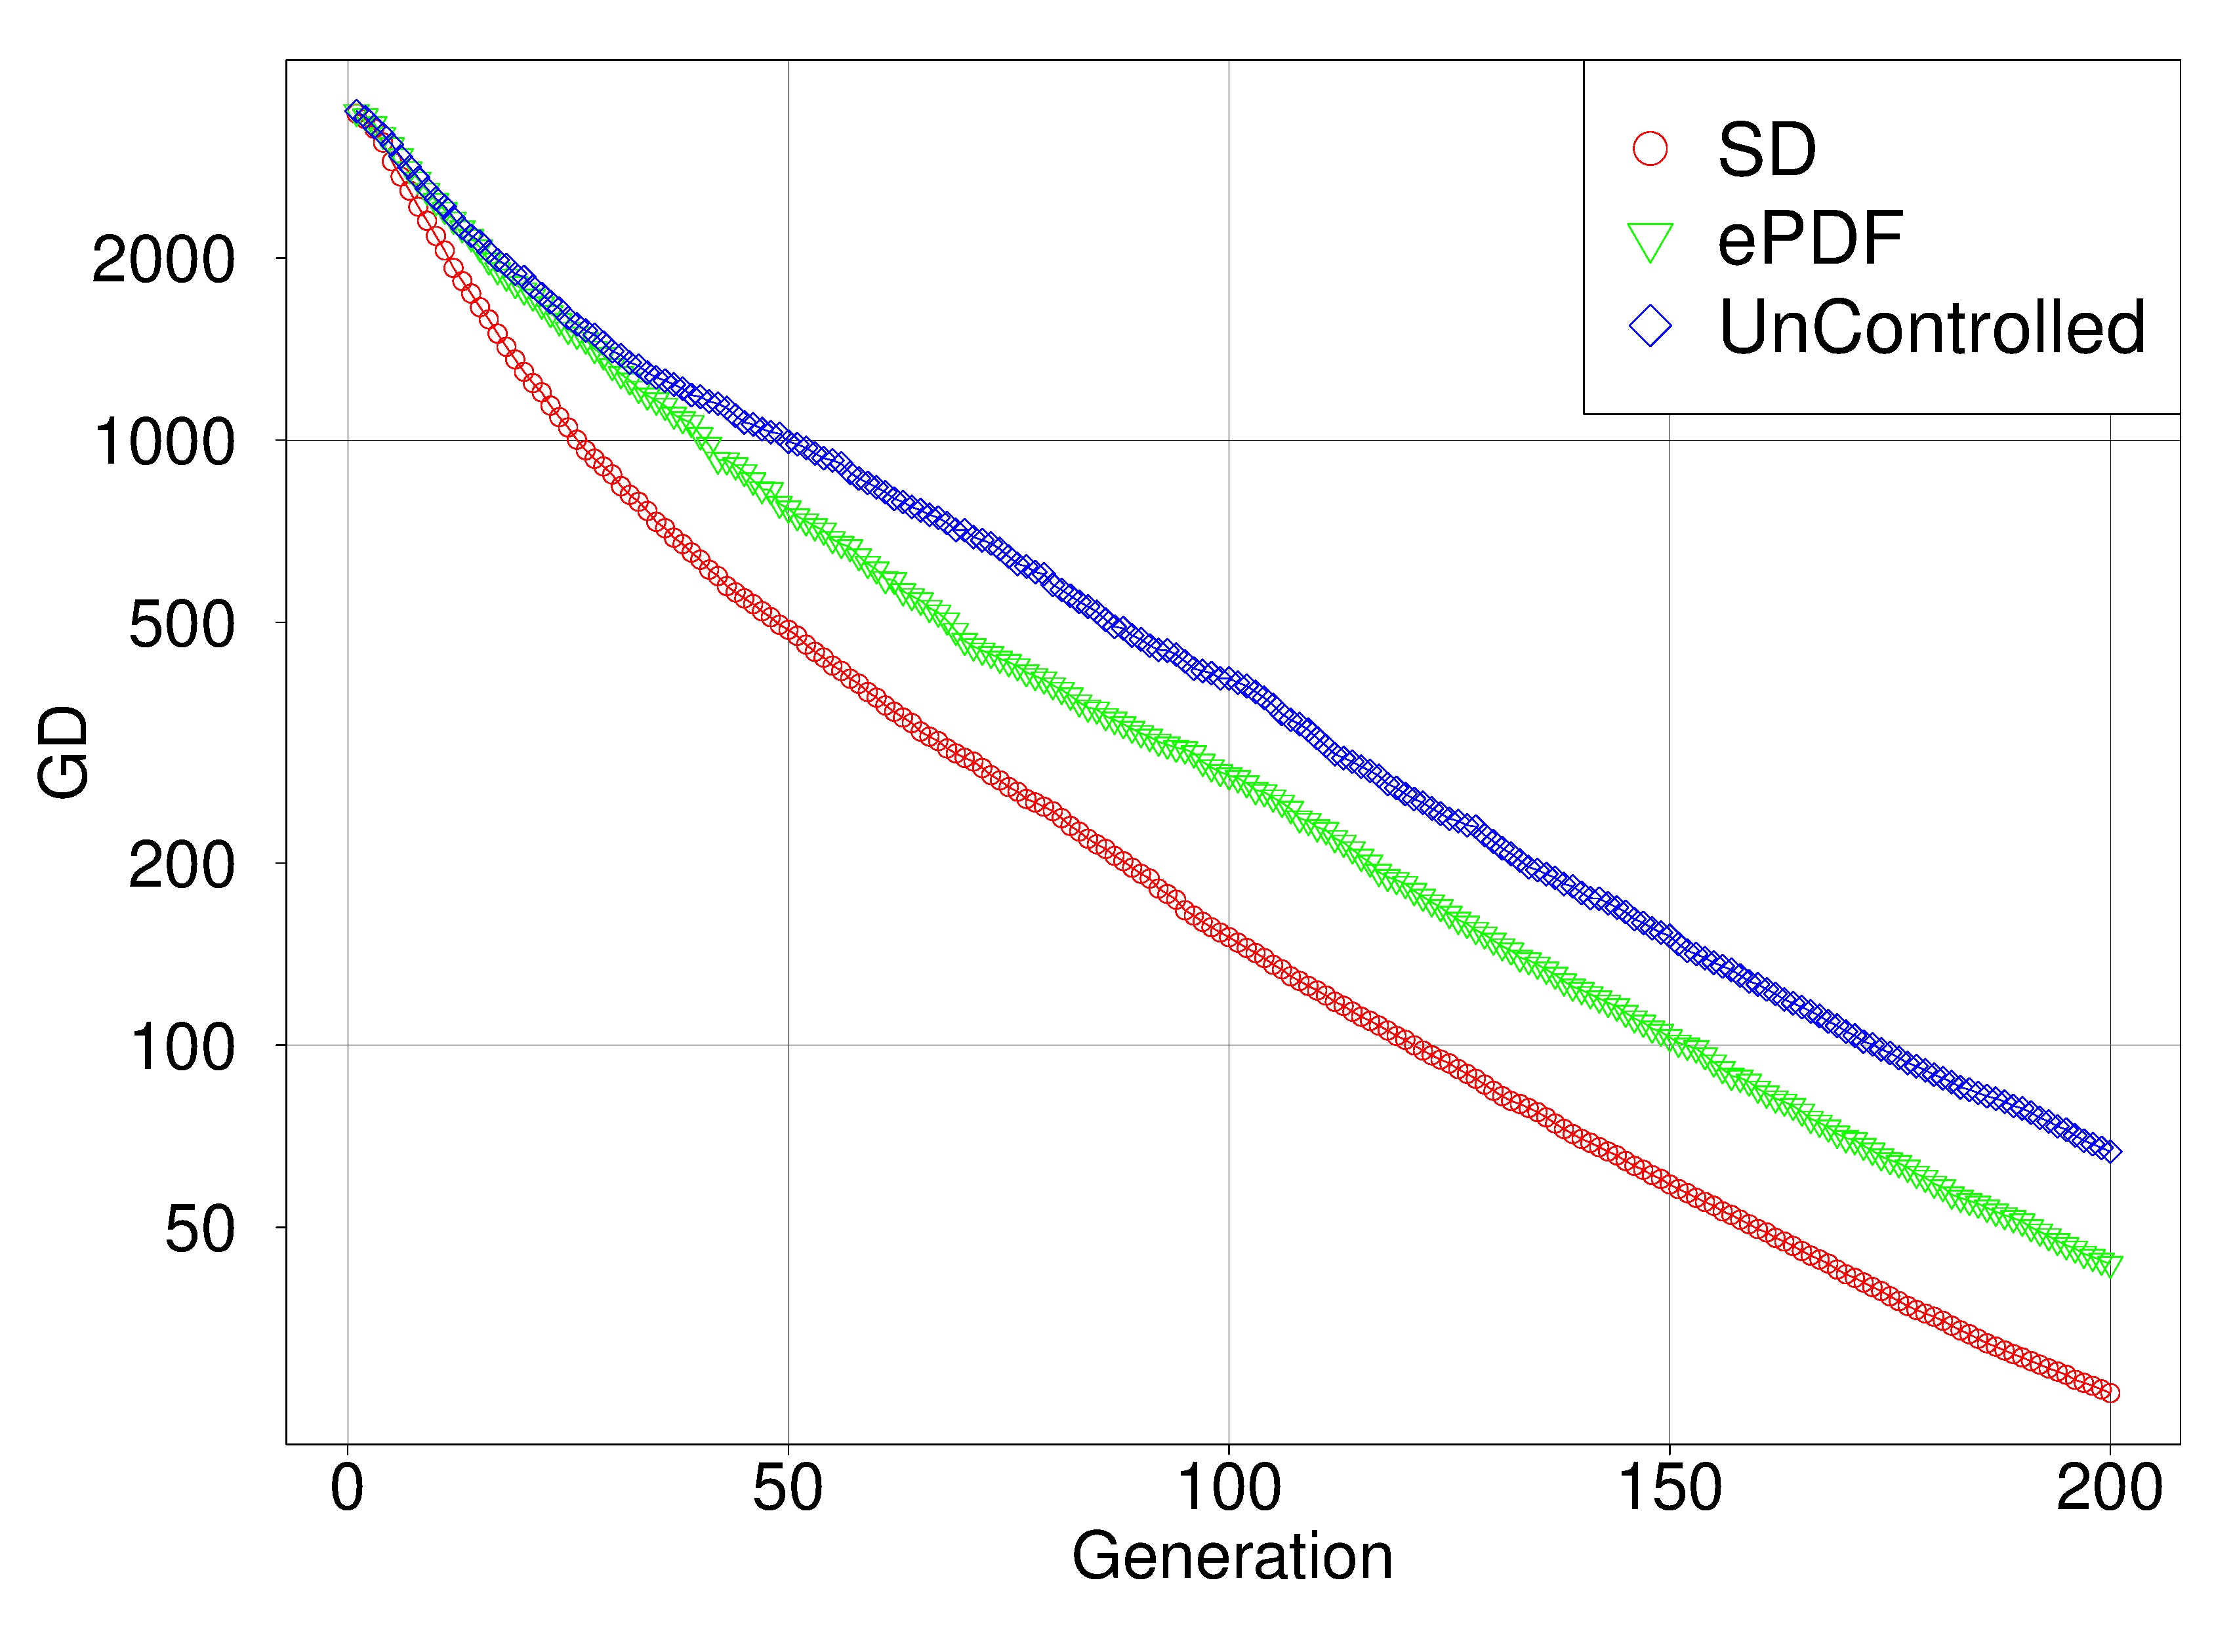
\includegraphics[width=1\linewidth]{../figures/DTLZ3_GD.eps}
\caption{適応的離散化手法を用いた場合と用いない場合のDTLZ3におけるGDの推移}
\label{dtlz3_gd_transition}
\end{minipage}
\begin{minipage}{0.49\hsize}
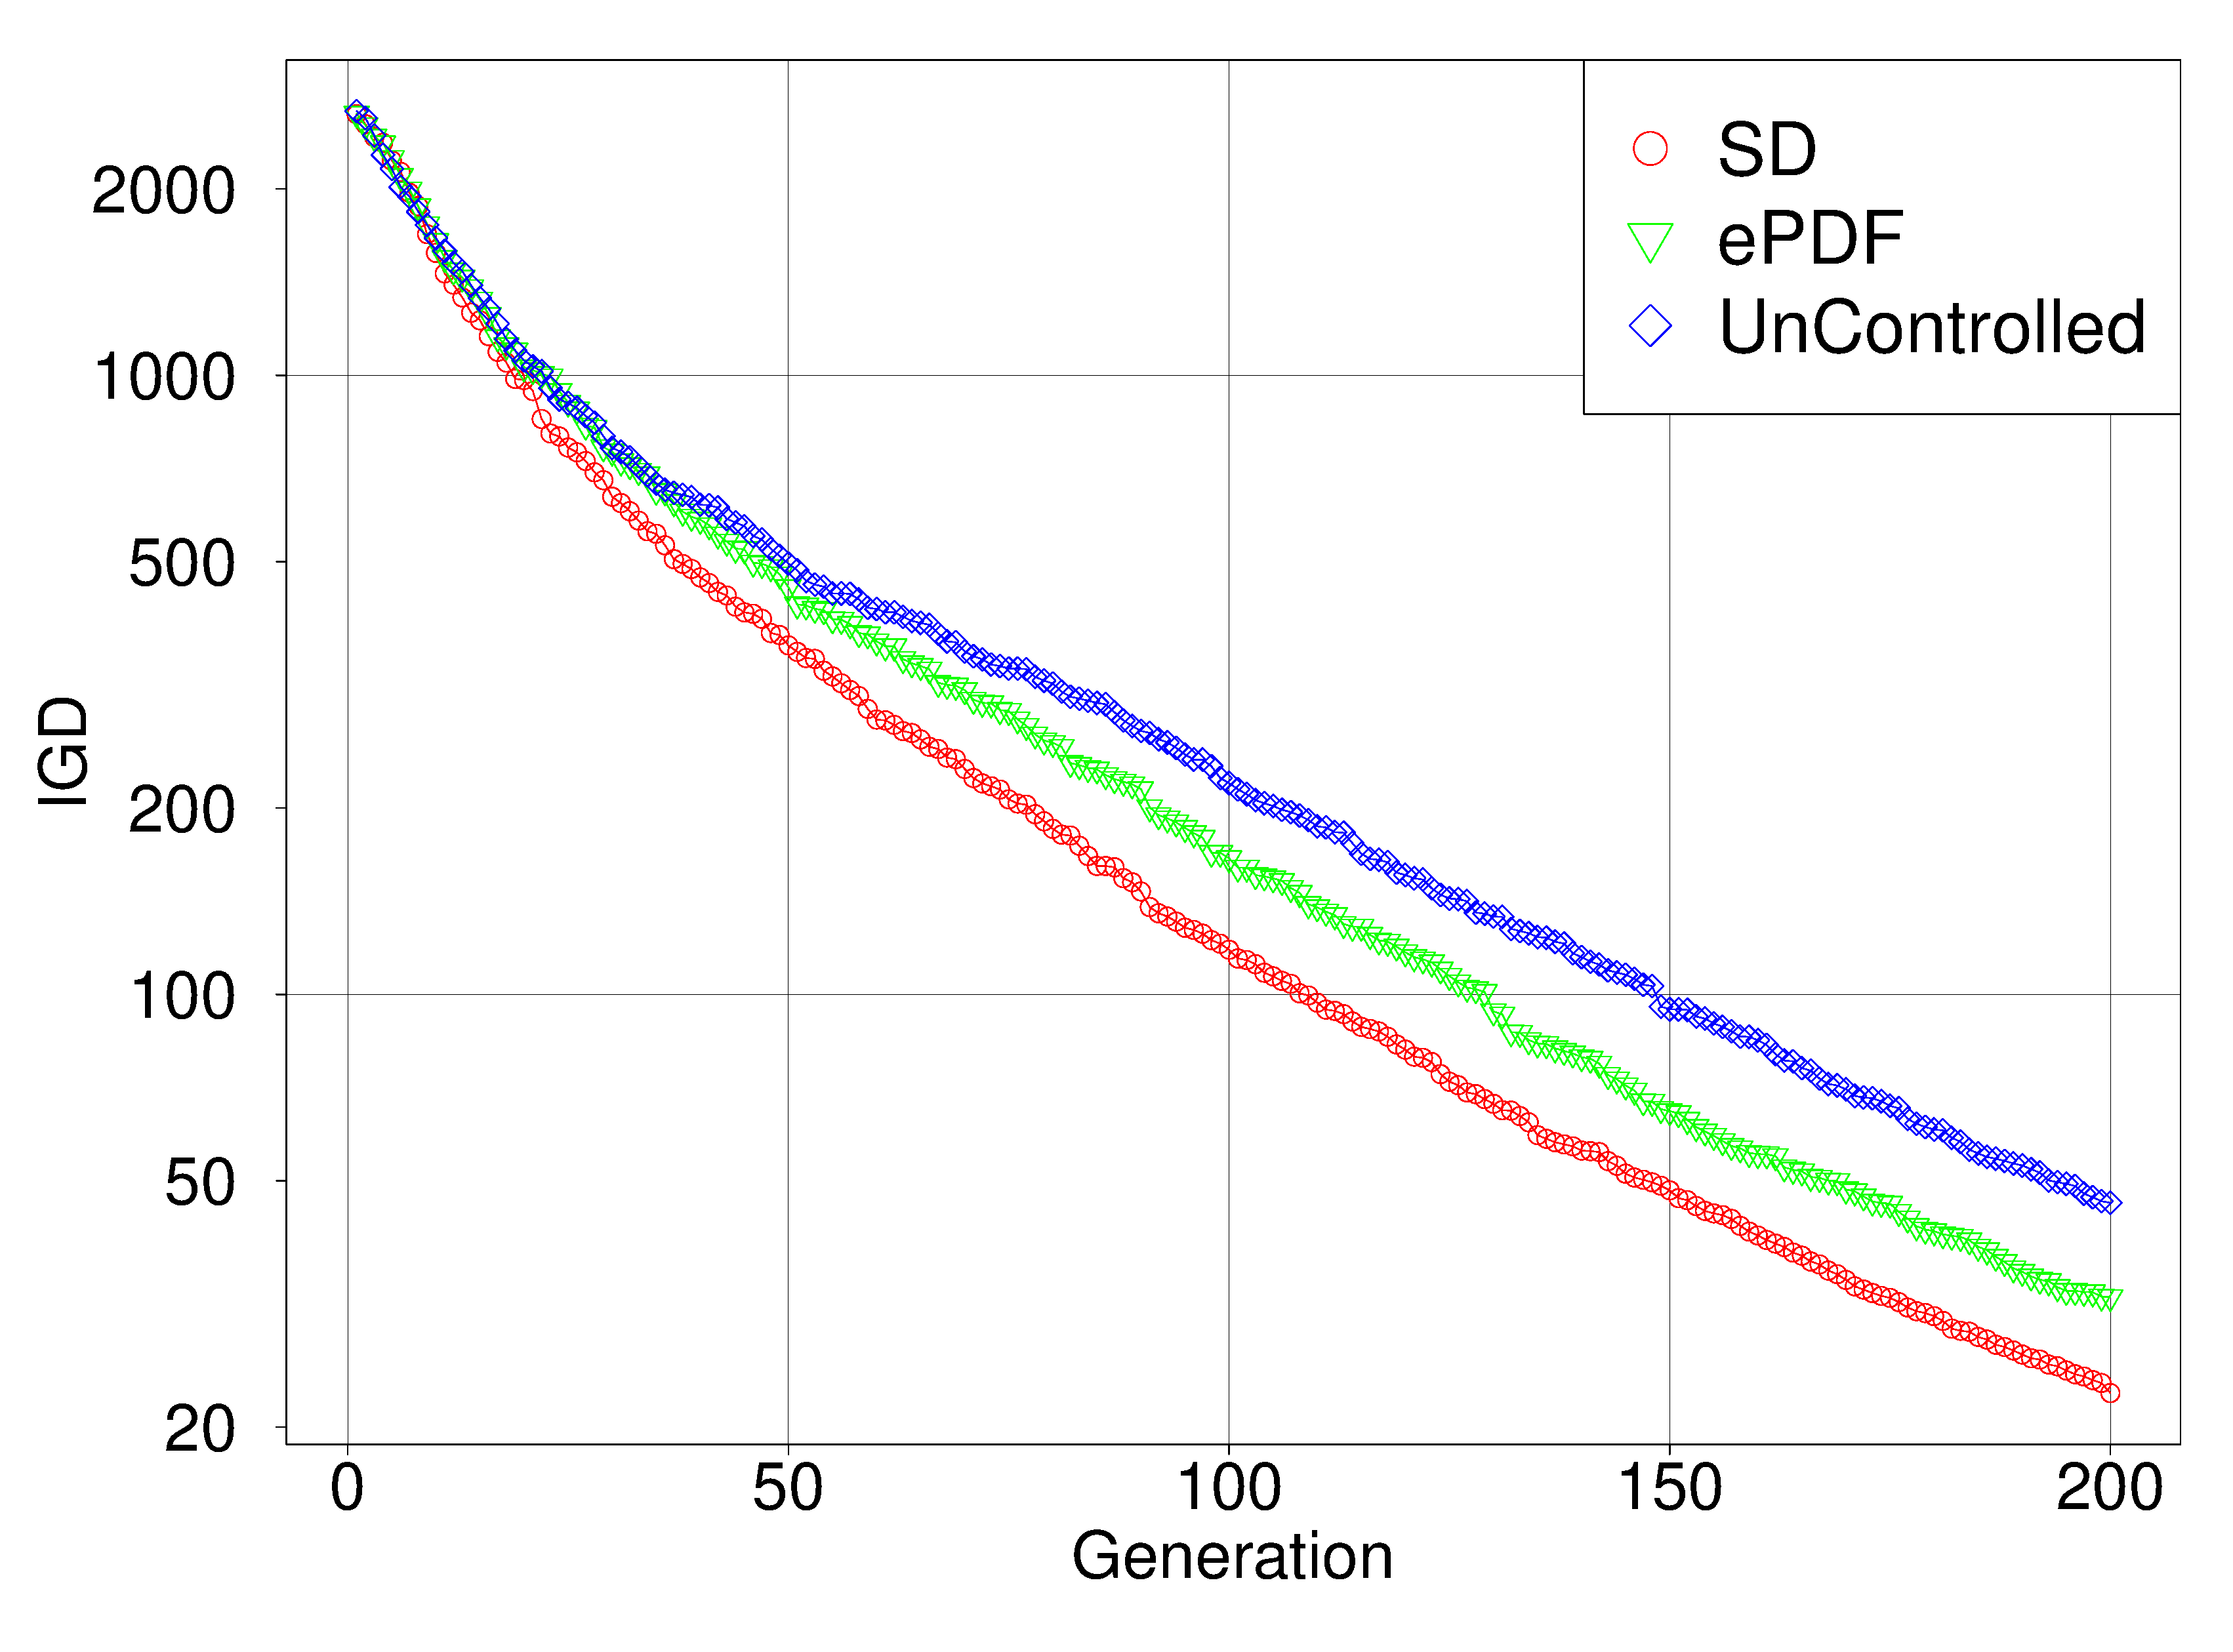
\includegraphics[width=1\linewidth]{../figures/DTLZ3_IGD.eps}
\caption{適応的離散化手法を用いた場合と用いない場合のDTLZ3におけるIGDの推移}
\label{dtlz3_igd_transition}
\end{minipage}
\end{tabular}
\end{figure*}

\begin{figure*}[htbp]
\begin{tabular}{cc}
\begin{minipage}{0.33\hsize}
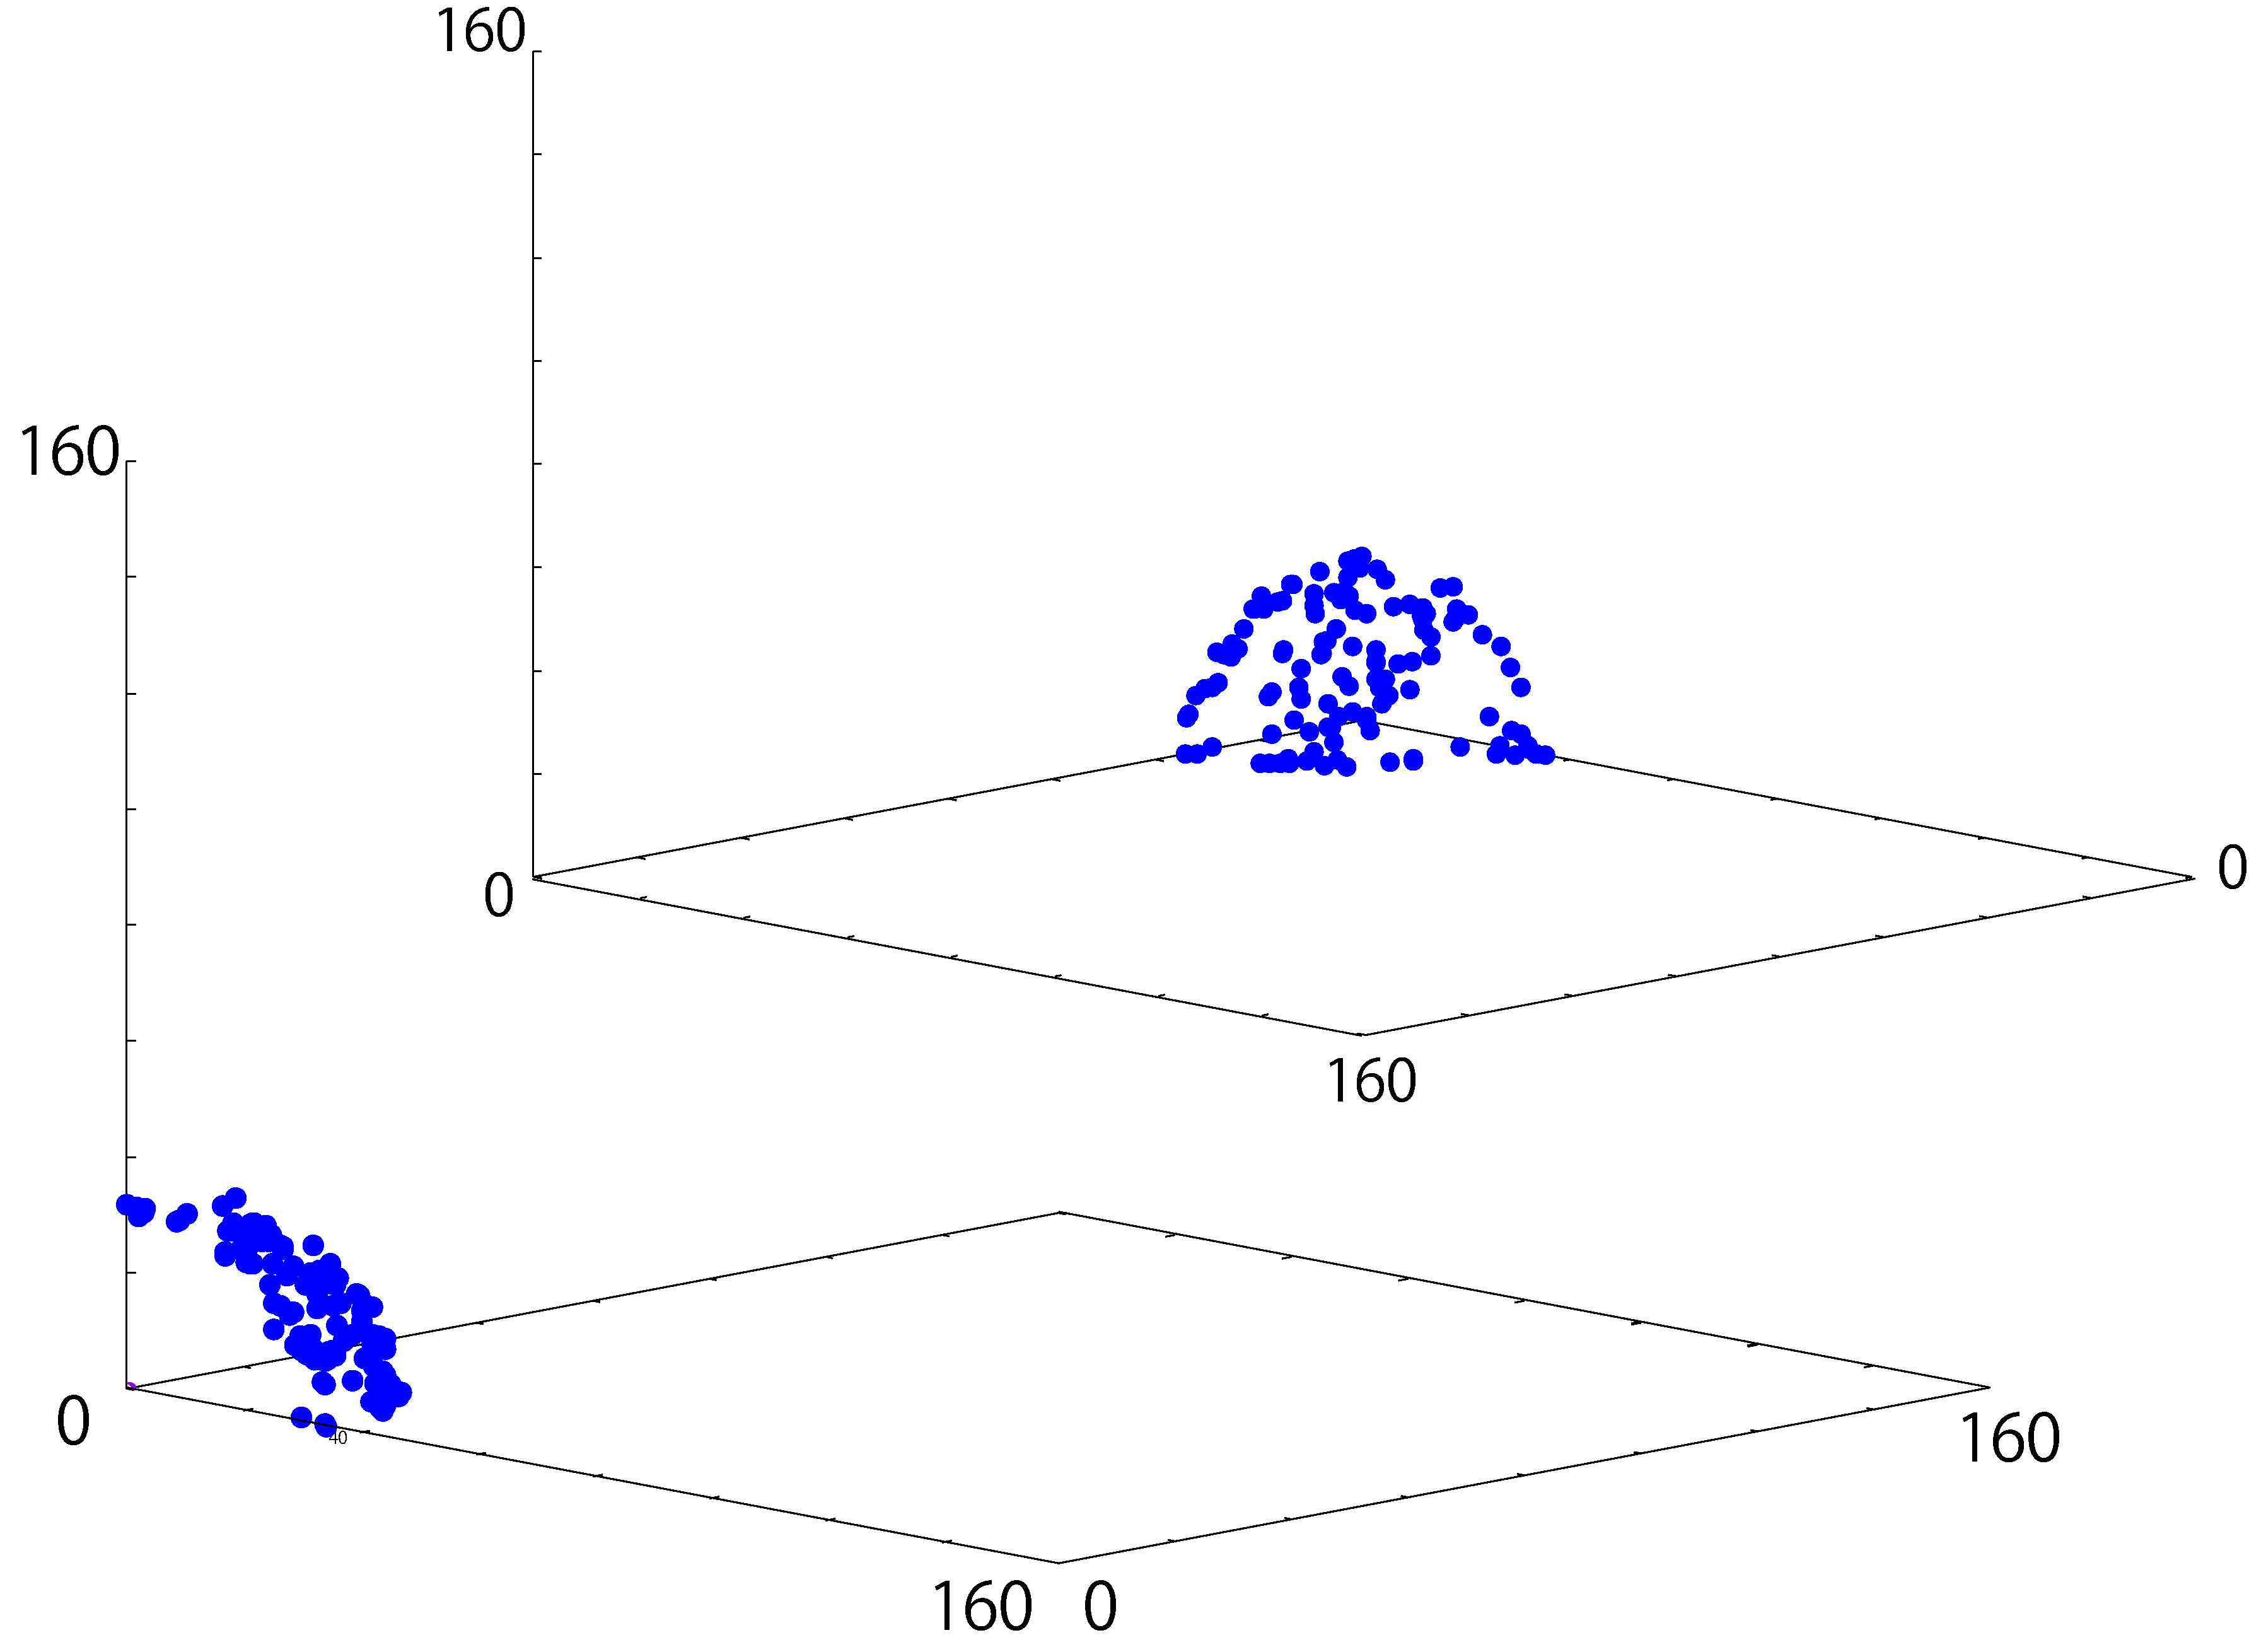
\includegraphics[width=1\linewidth]{../figures/dtlz3_sd_double.pdf}
\begin{center}
{\footnotesize (a) SD}
\end{center}
\end{minipage}
\begin{minipage}{0.33\hsize}
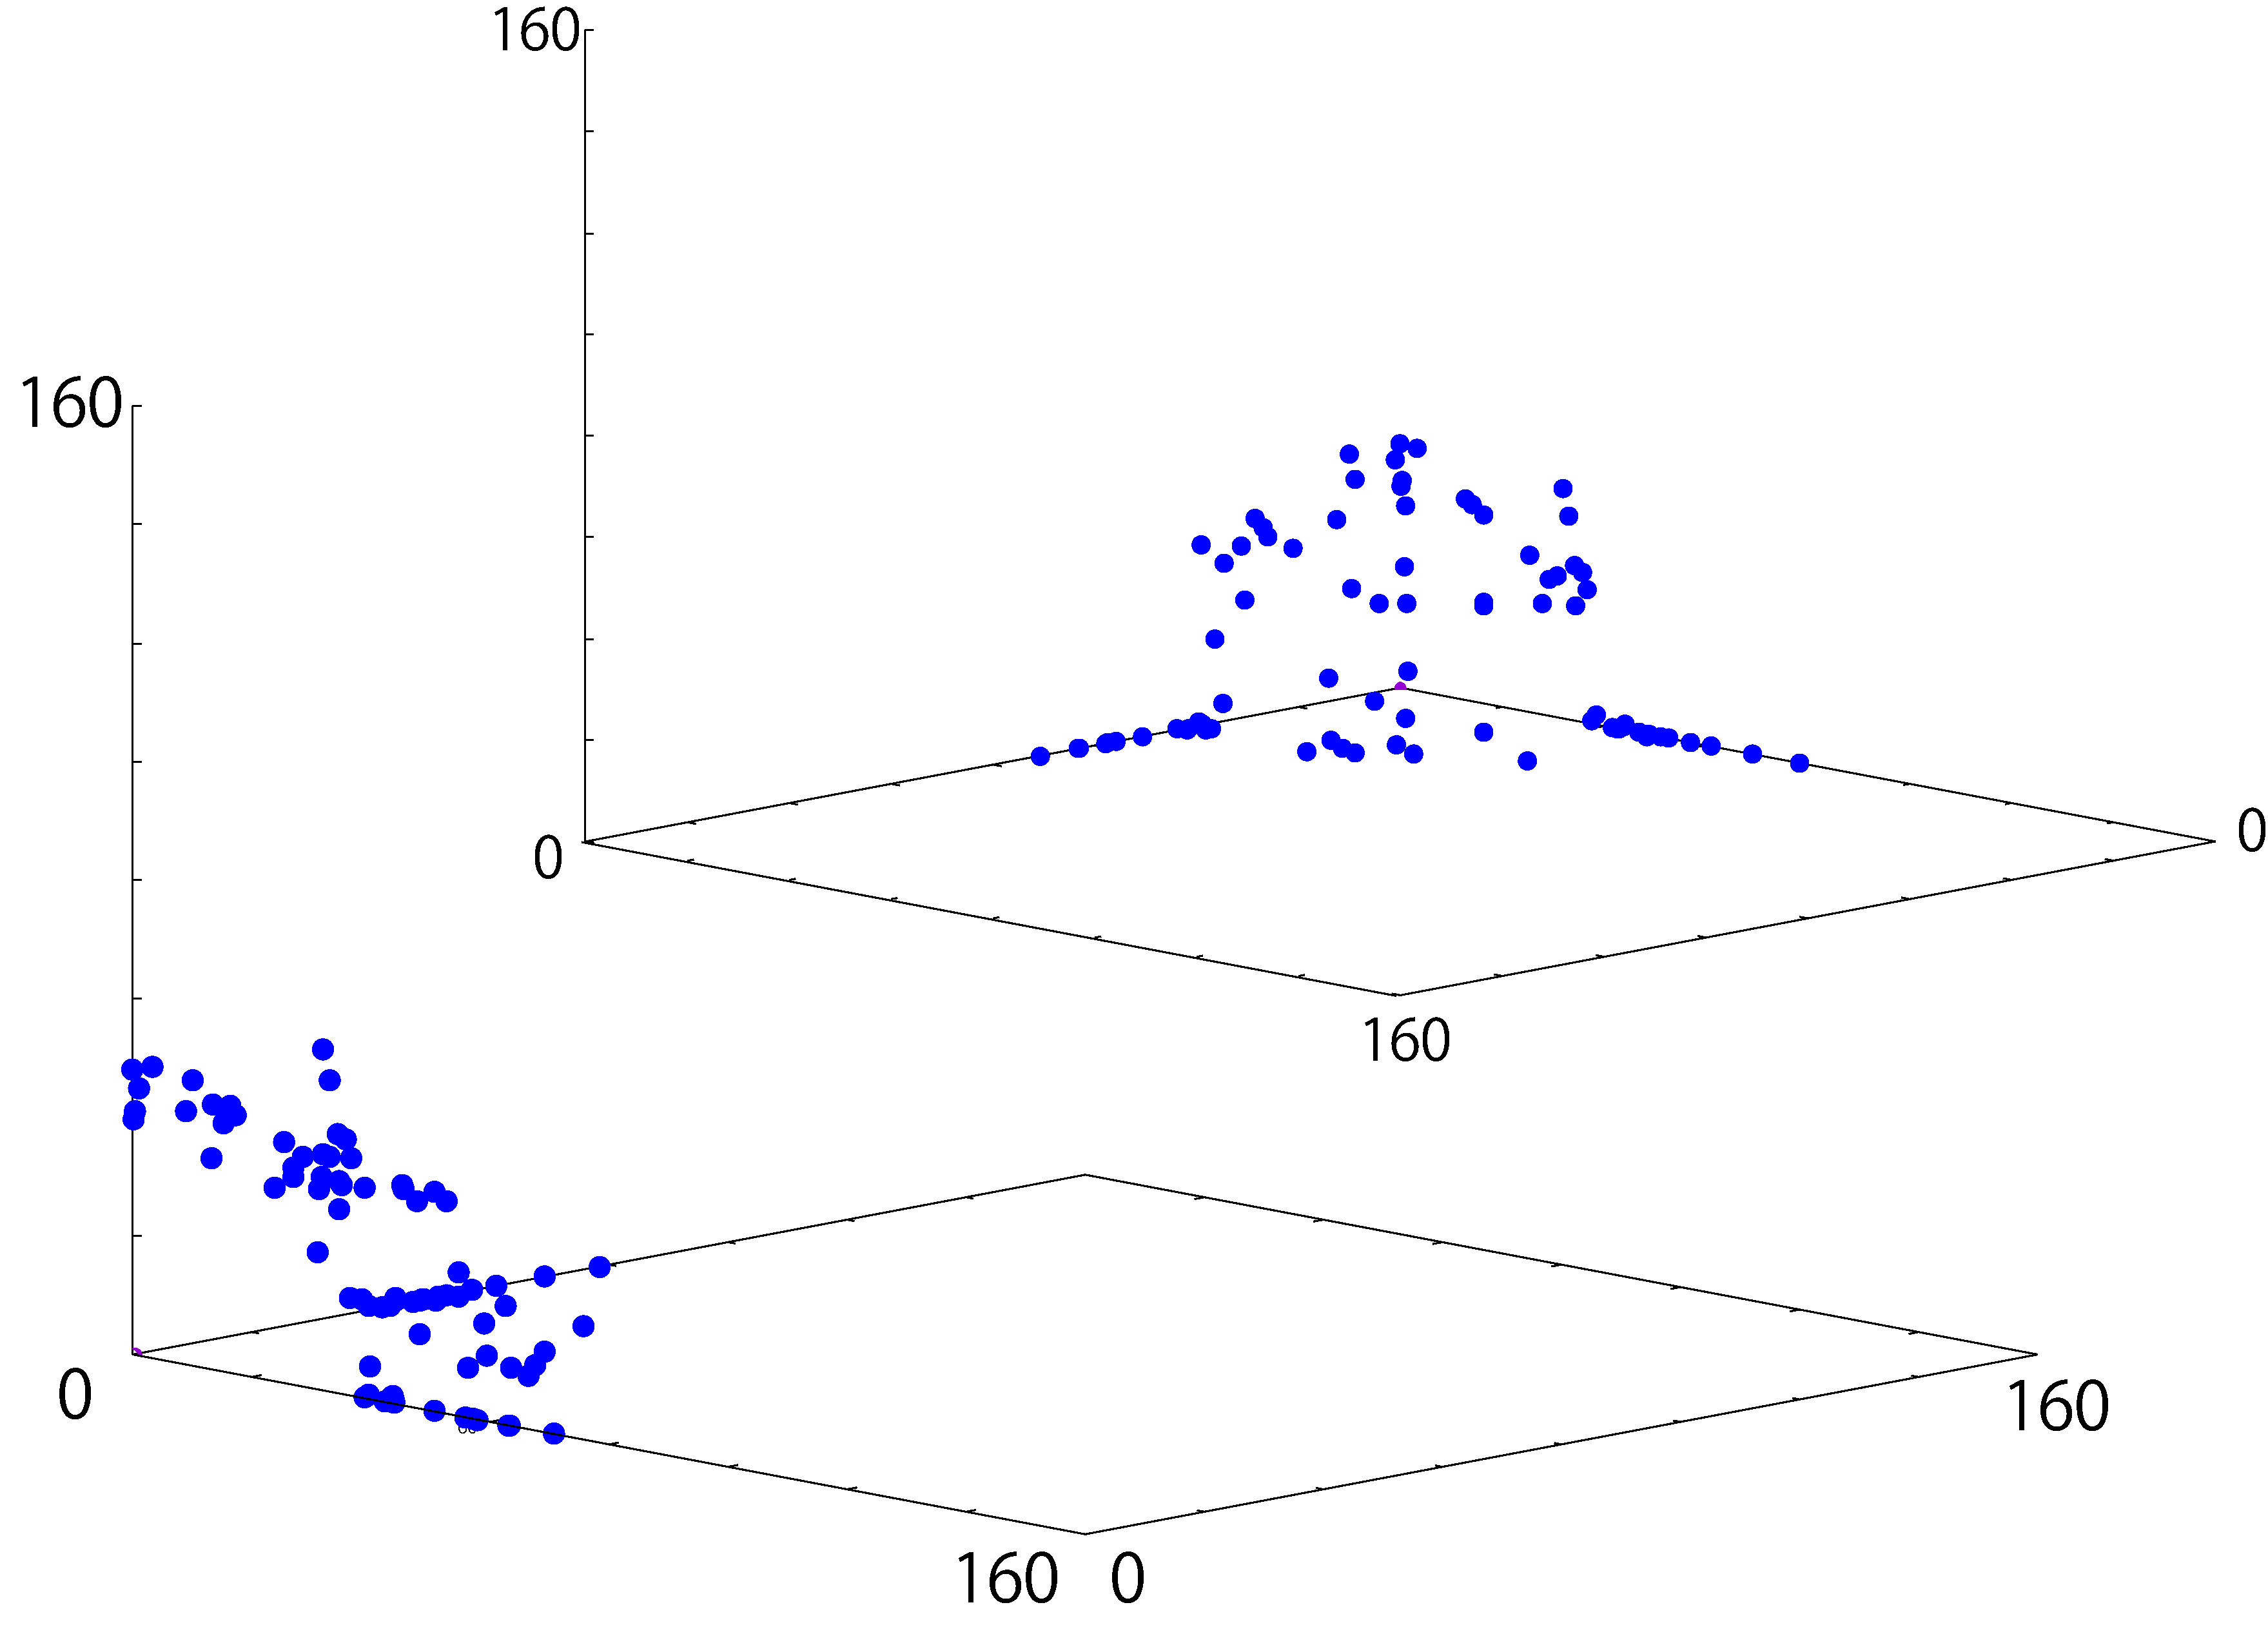
\includegraphics[width=1\linewidth]{../figures/dtlz3_kde_double.pdf}
\begin{center}
{\footnotesize (b) ePDF}
\end{center}
\end{minipage}
\begin{minipage}{0.33\hsize}
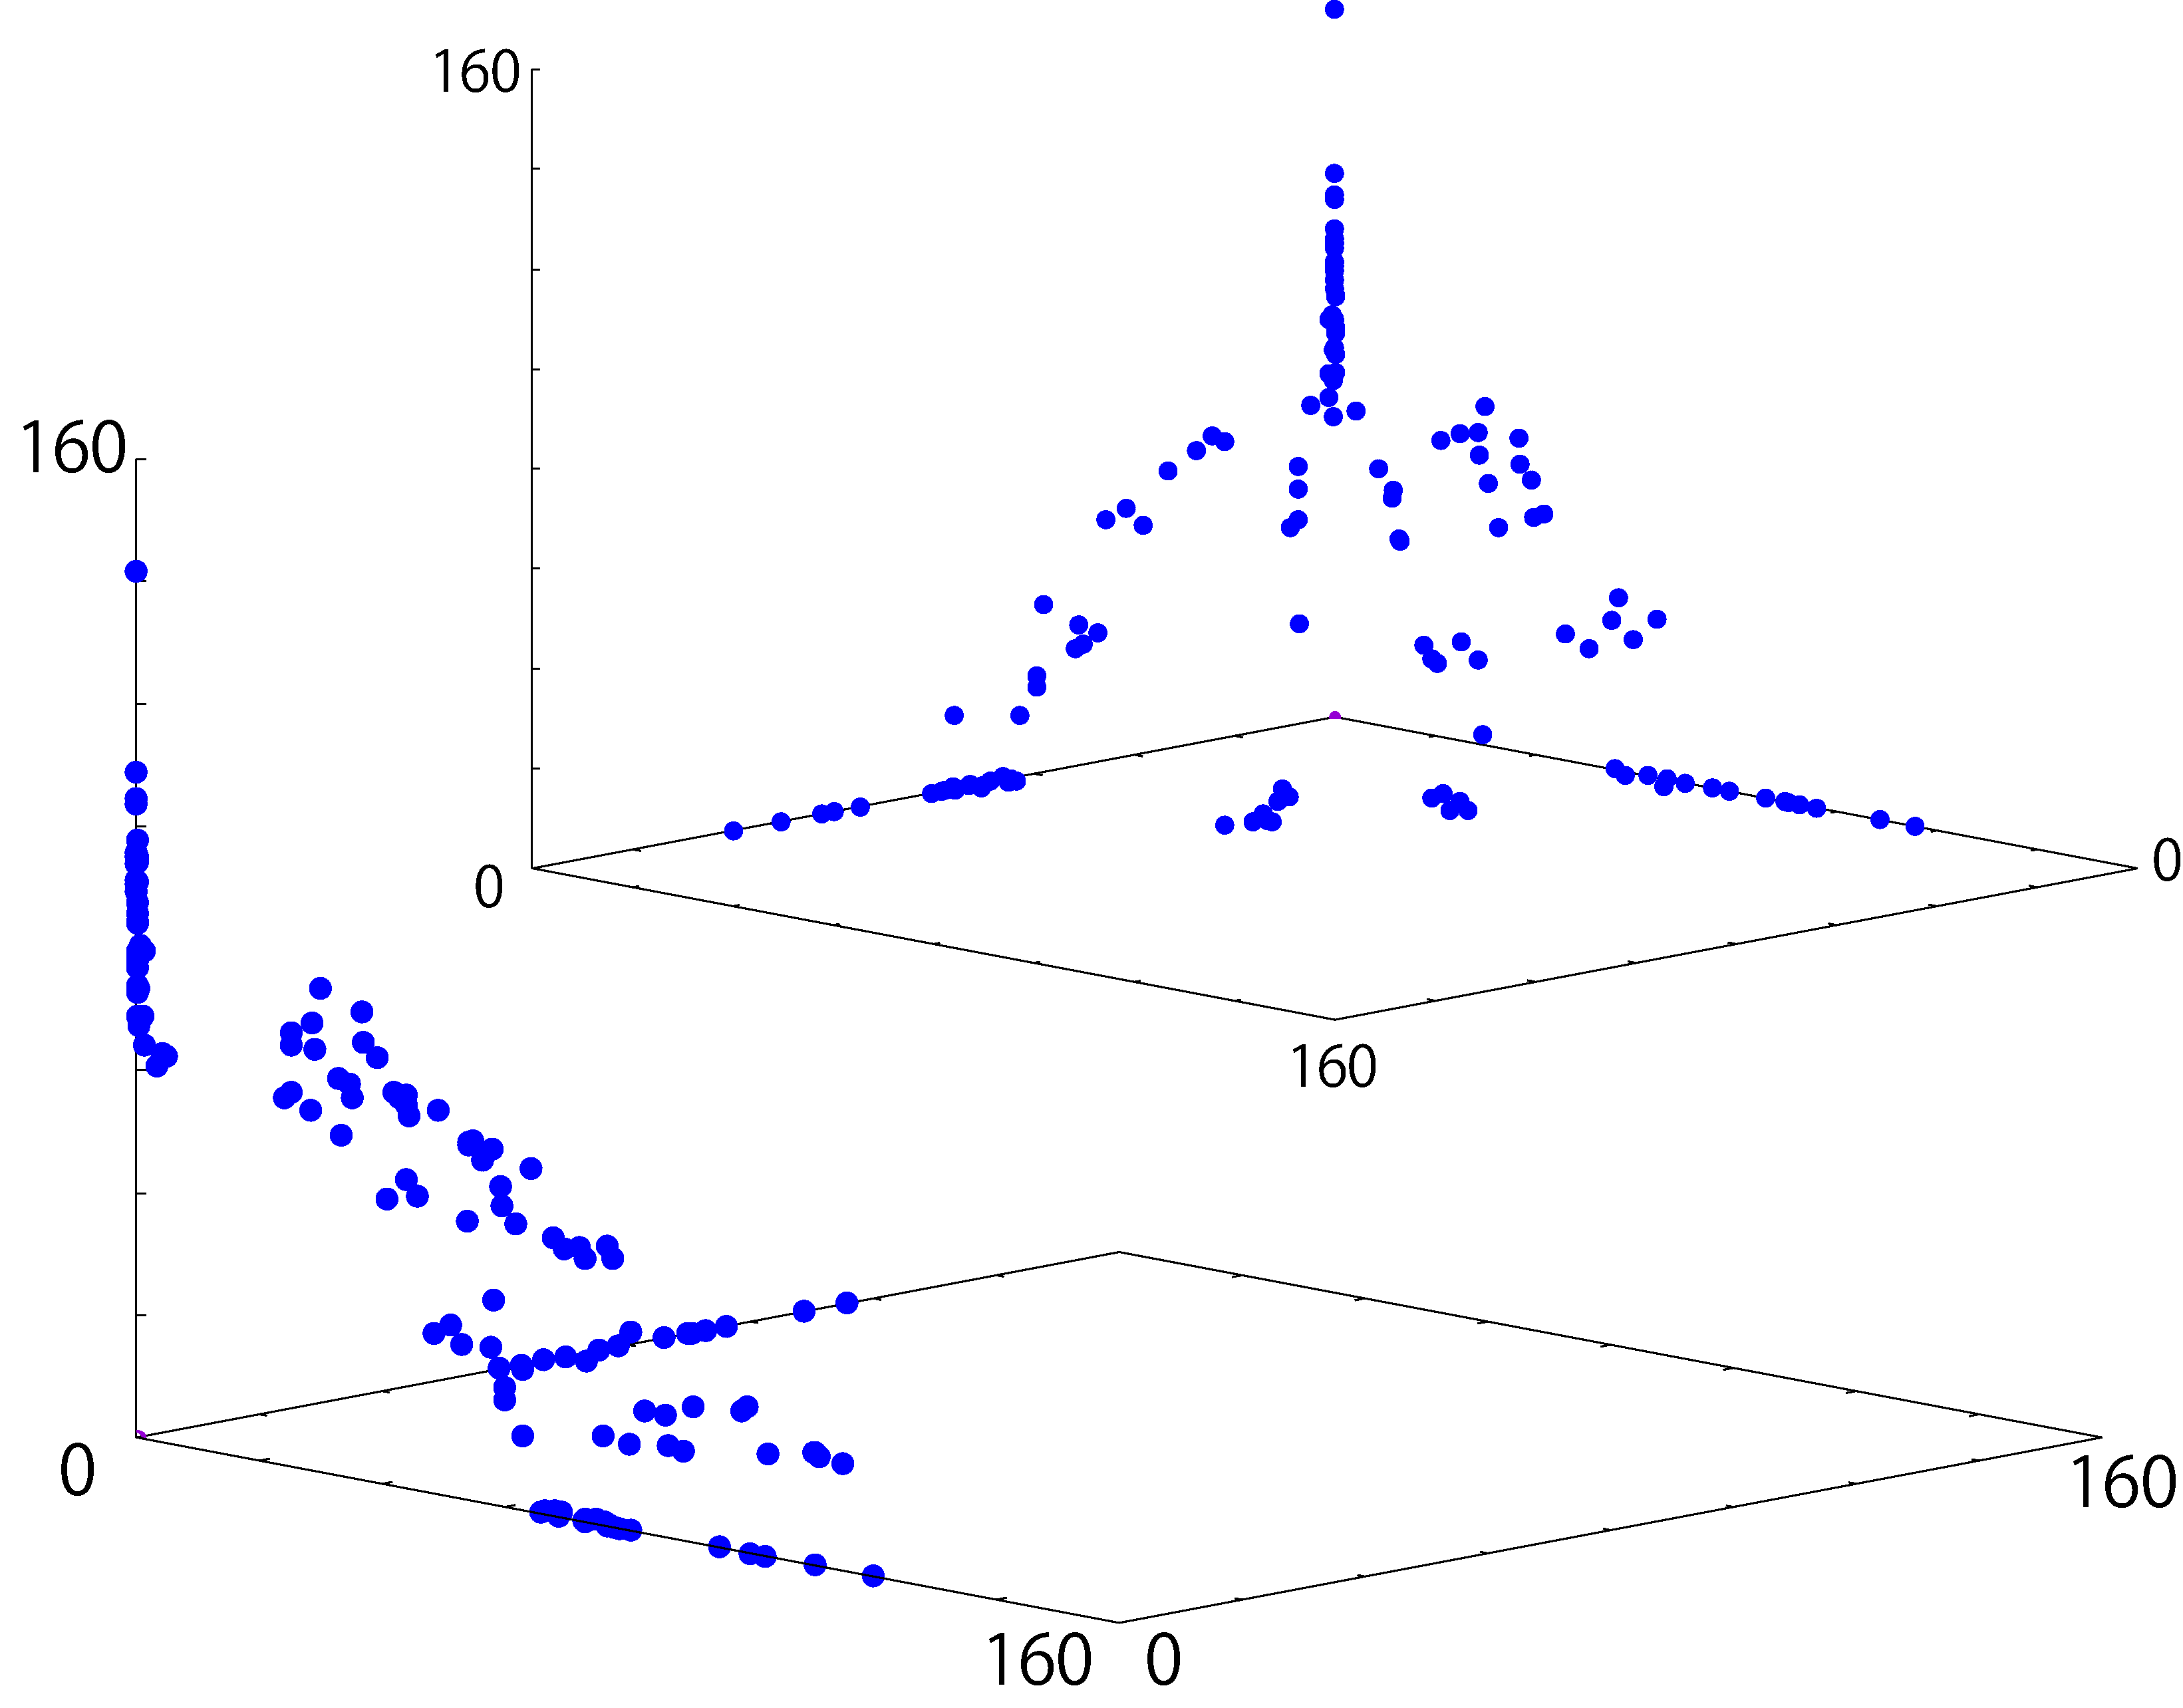
\includegraphics[width=1\linewidth]{../figures/dtlz3_uc_double.pdf}
\begin{center}
{\footnotesize (c) 制御なし}
\end{center}
\end{minipage}
\end{tabular}
\caption{適応的離散化手法を用いた場合と用いない場合のDTLZ3における非劣解の分布}
\label{fig:nondoms}
\end{figure*}

\begin{figure*}[!h]
\begin{minipage}{0.38\hsize}
\vspace{-0.2in}
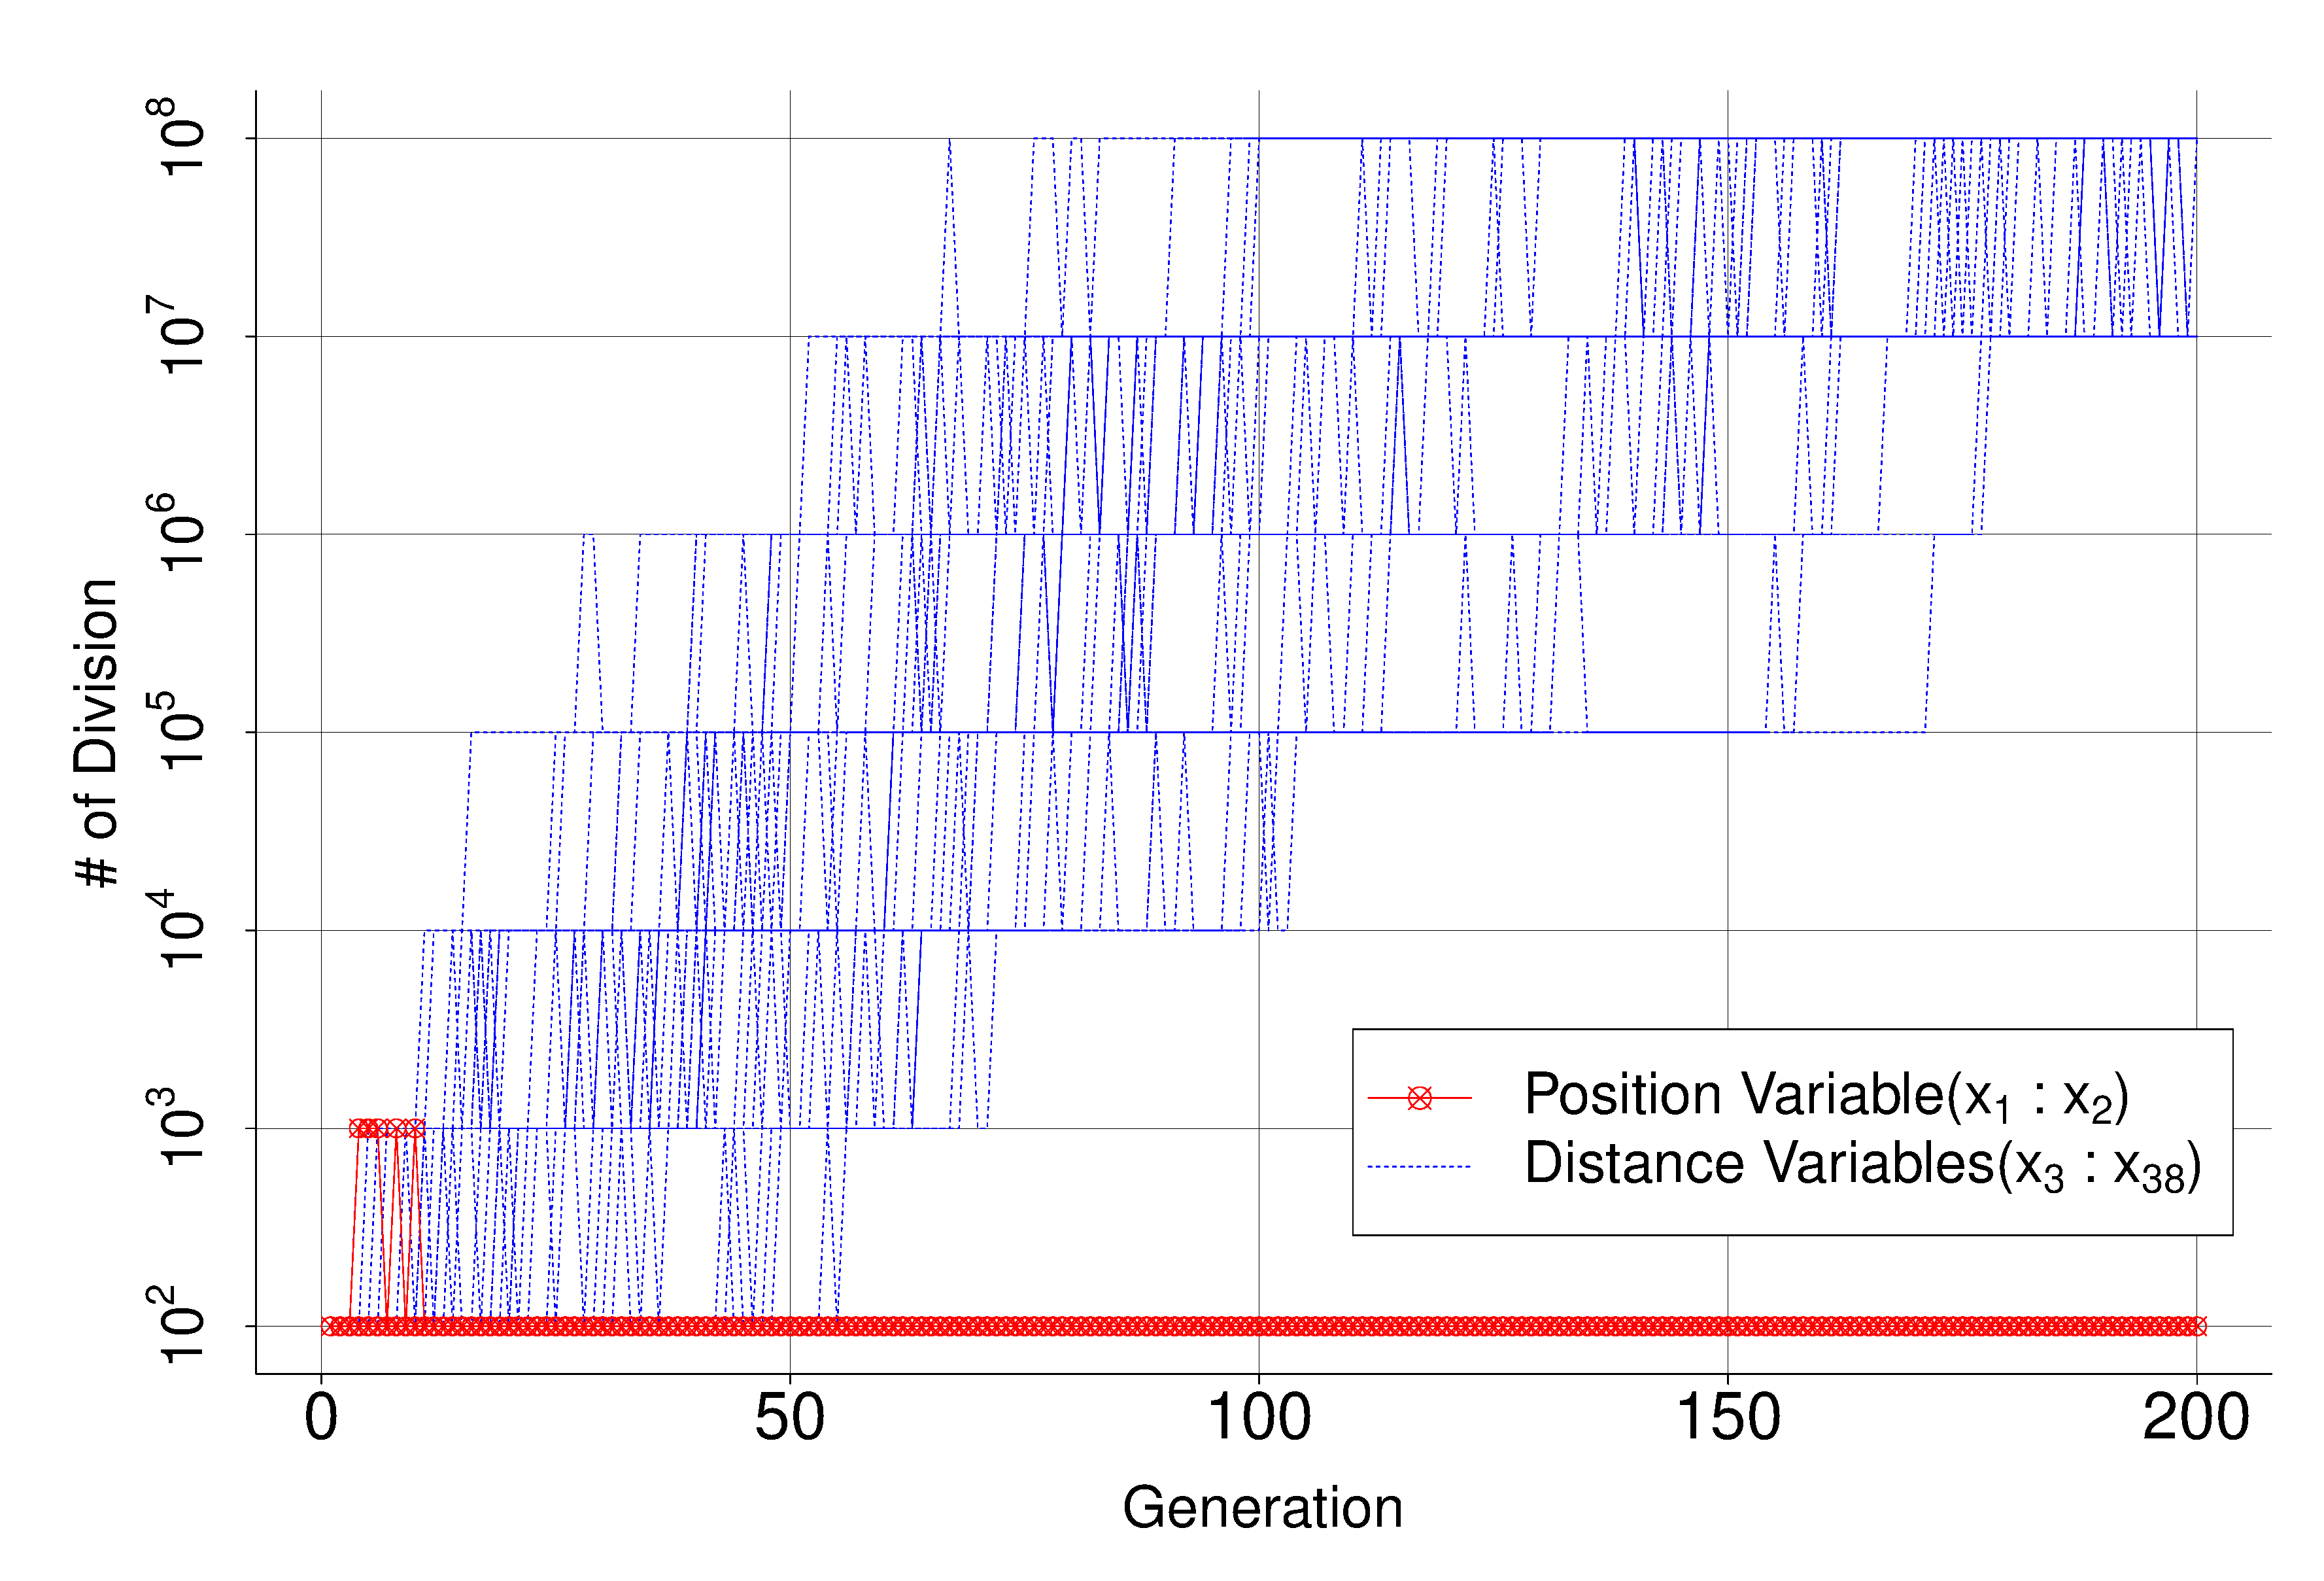
\includegraphics[width=1\linewidth]{../figures/DTLZ3_digit_trend.eps}\\
\\
\caption{SDを用いた場合のDTLZ3における各設計変数の分割数の世代ごとの推移}
\label{digi_trans}
\end{minipage}
\begin{minipage}{0.61\hsize}
\begin{minipage}{0.49\hsize}
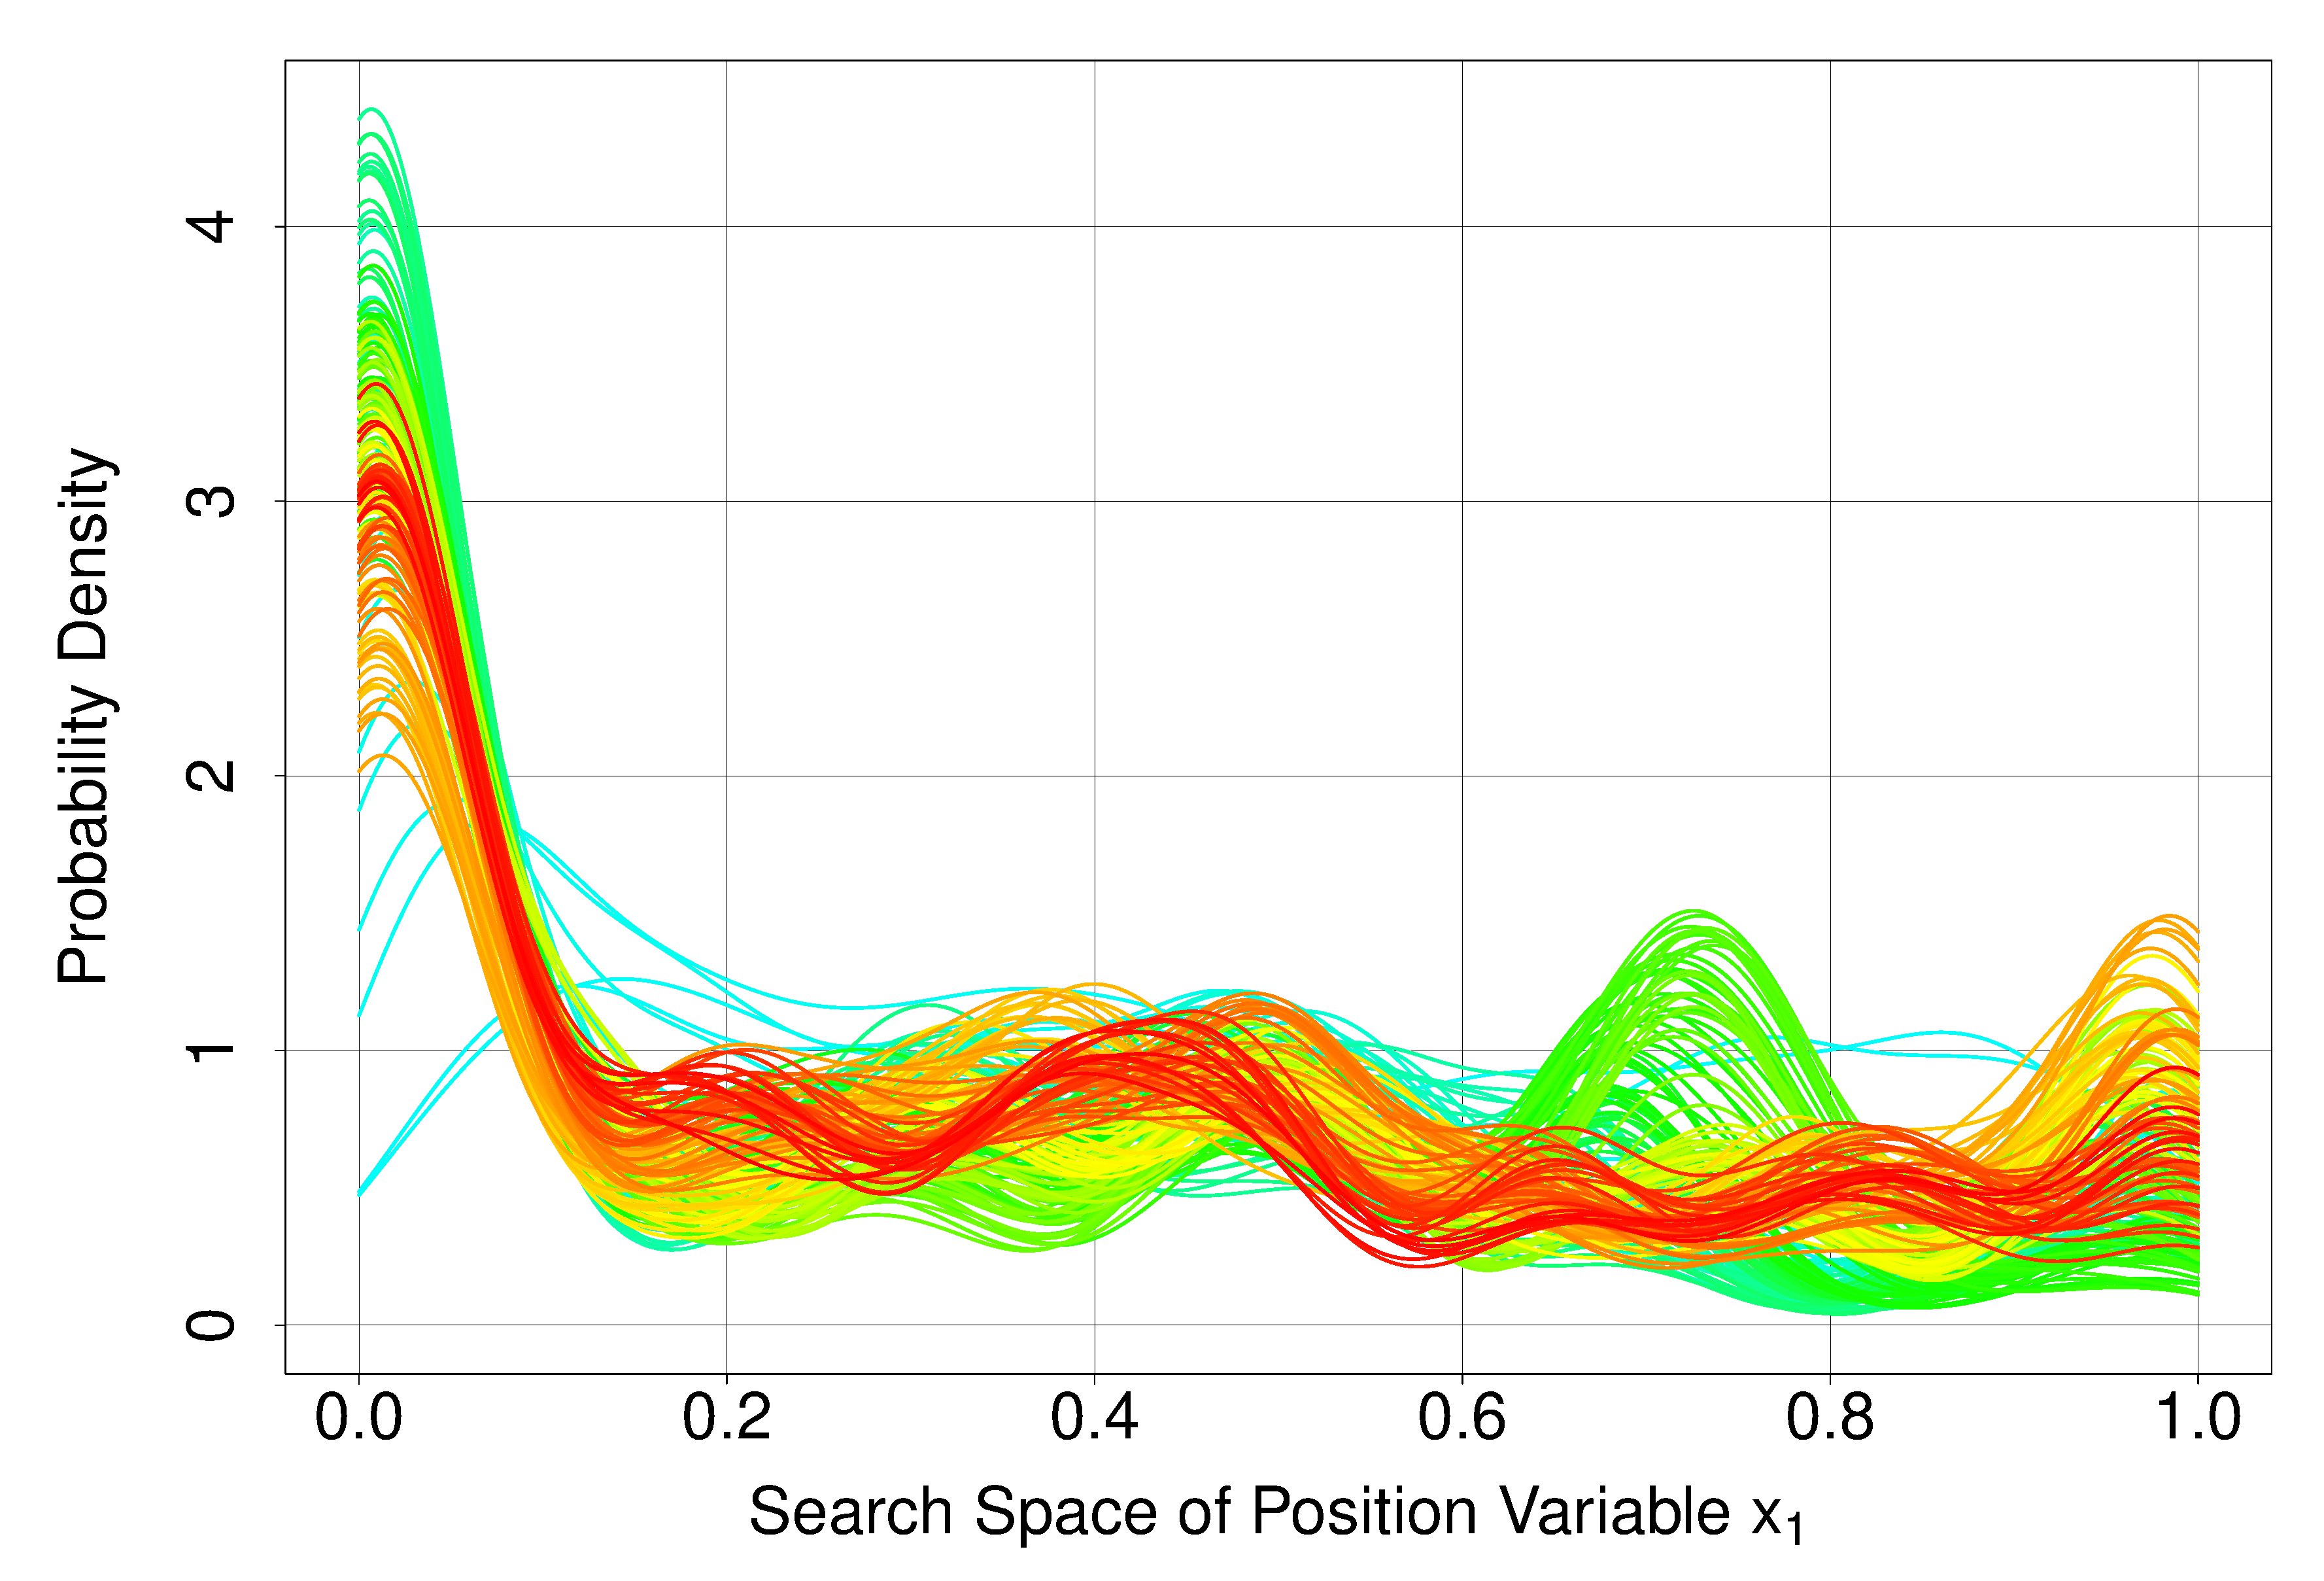
\includegraphics[width=1\linewidth]{../figures/DTLZ3_var1_pdf_trend.eps}\\
\centering
\hspace{0.2in} \includegraphics[width=0.8\linewidth]{../figures/color_bar.eps}
\begin{center}
{\footnotesize (a) 位置変数$x_1$における推定された確率密度関数の推移}
\end{center}
\end{minipage}
\begin{minipage}{0.49\hsize}
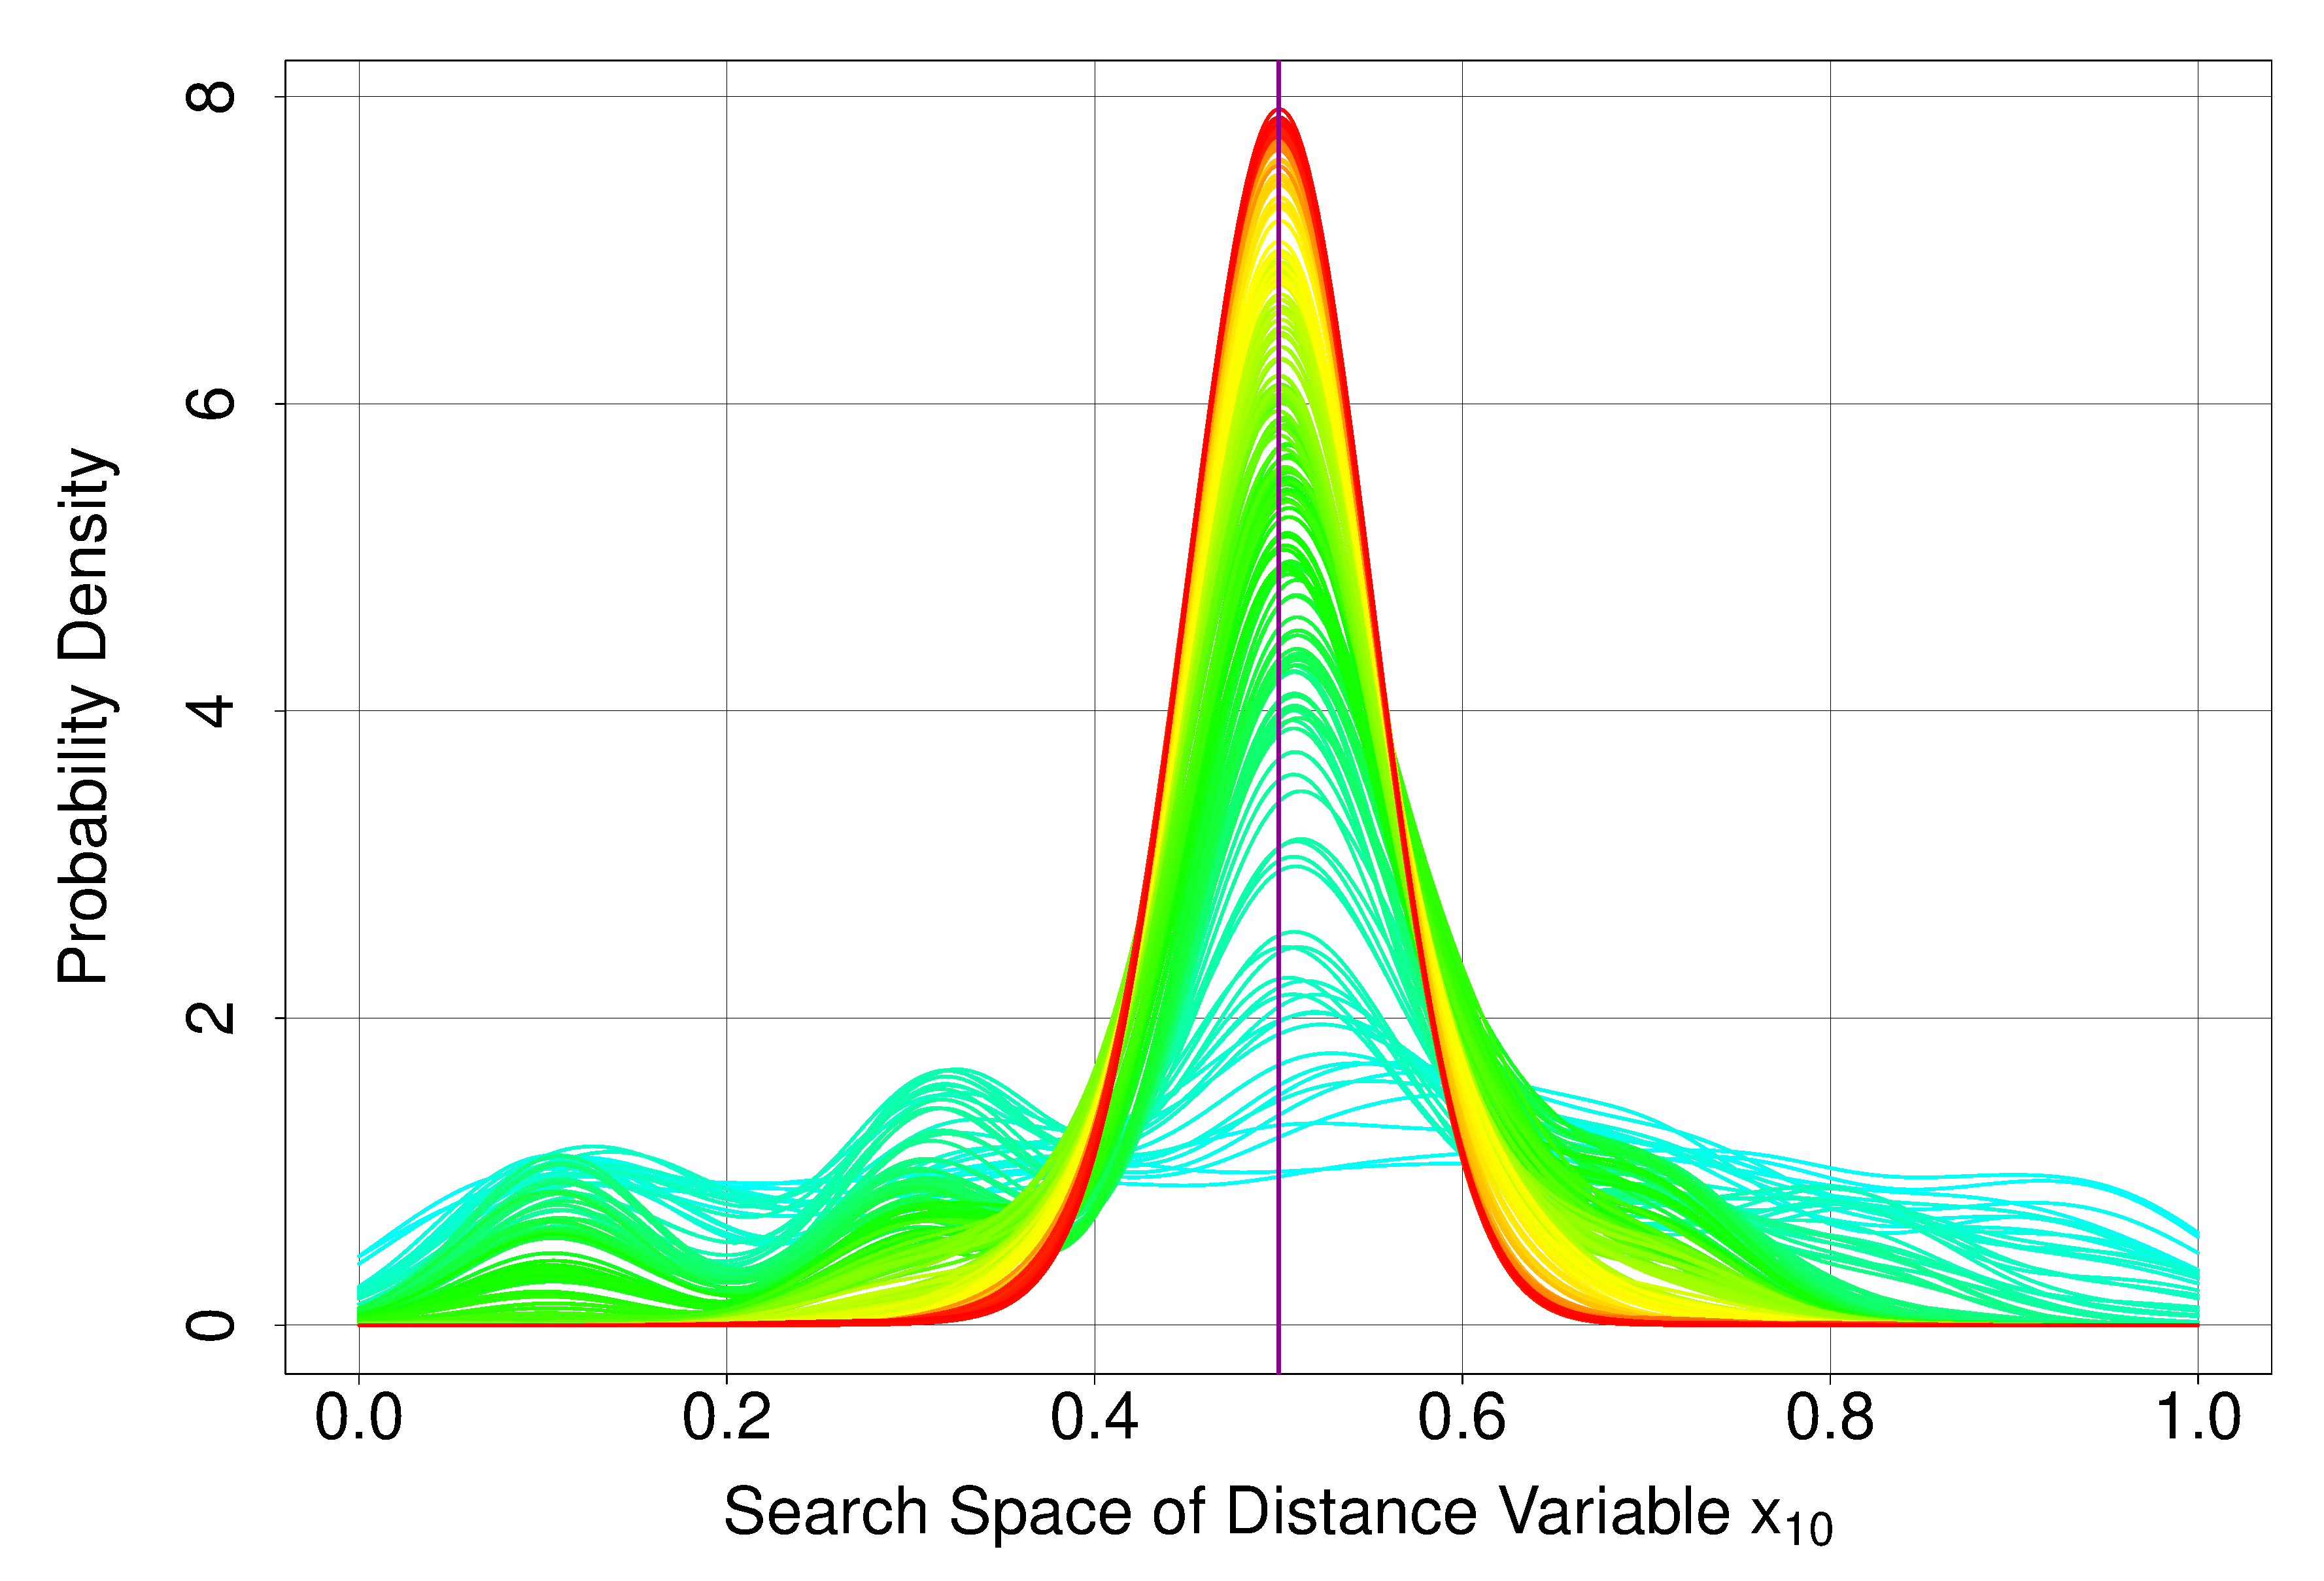
\includegraphics[width=1\linewidth]{../figures/DTLZ3_var10_pdf_trend.eps}\\
\centering
\hspace{0.2in} \includegraphics[width=0.8\linewidth]{../figures/color_bar.eps}
\begin{center}
{\footnotesize (b) 距離変数$x_{10}$における推定された確率密度関数の推移}
\end{center}
\end{minipage}
\caption{ePDFを用いた場合のDTLZ3における推定された確率密度関数の世代ごとの推移}
\label{pdf_trans}
\end{minipage}
\label{fig:nondom_sol}
\end{figure*}

\clearpage

\Figref{pdf_trans}は,ePDFを用いた場合に各世代におけるある設計変数空間の分布について推定された確率密度関数を示しており,(a)は位置変数である$x_1$,(b)は距離変数である$x_{10}$について得られた確率密度関数を示している.
縦軸は確率密度,横軸は設計変数空間を正規化空間に射影した際の探索空間を示しており[0,1]の範囲であり,確率密度関数の色は推定された世代を示している.
また,\Figref{pdf_trans}(b)における図中の紫の縦線は真の最適値を示している.
ePDFを用いた適応的離散化では,確率密度が高いほど細かく離散化が行われる.
\Figref{pdf_trans}(a)より,位置変数$x_1$では世代を経るごとに0付近の確率密度が高い値となっていることから,0付近の解は細かく離散化されていることが分かる.
位置変数が0付近に生成された場合,目的関数空間では極付近に解が生成されるため,非劣解になりやすく生存しやすい.
そのため,0付近に分布が集中したものと考えられる.
しかしながら,極付近の解は進化の妨げとなるDRSsとなる可能性が高く,0付近の解を細かく離散化してしまうことでDRSsの発生を誘発してしまっている可能性がある.
したがって,ePDFはSDに比べ解の収束性が低下しているものと考えられる.
\Figref{pdf_trans}(b)より,距離変数$x_{10}$は世代を経るごとに0.5付近の確率密度が高い値となっていることから,0.5付近の解は細かく離散化されていることが分かる.
DTLZ3における距離変数の真の最適値は0.5であることから,最適解付近を細かく離散化し,最適化付近を細かく探索できていることが分かる.
このように,最適化付近は細かく離散化を行い,その他の領域では粗い離散化が行われたことが,離散化を行わなかった場合と比べ収束性が向上した一因であると考えられる.
また,\Figref{pdf_trans}(b)の結果から,距離変数の探索においては期待したメカニズムが有効に機能していることが分かる.

\subsubsection{WFG7}

\Figref{wfg7_gd_transition},\ref{wfg7_igd_transition}はそれぞれWFG7においてSD,ePDFを用いた適応的離散化手法と離散化制御を用いなかった場合に得られたGD,IGDの平均値の推移を示している.
\Figref{wfg7_gd_transition},\ref{wfg7_igd_transition}を見ると,GD,IGDともに離散化制御を行わなかった場合が最も良く,次いでePDFが良い結果となっている.
この結果から,WFG7においては設計変数を離散化することで,探索効率が減少してしまう可能性があることが分かる.


\begin{figure*}[!ht]
\begin{tabular}{cc}
\begin{minipage}{0.49\hsize}
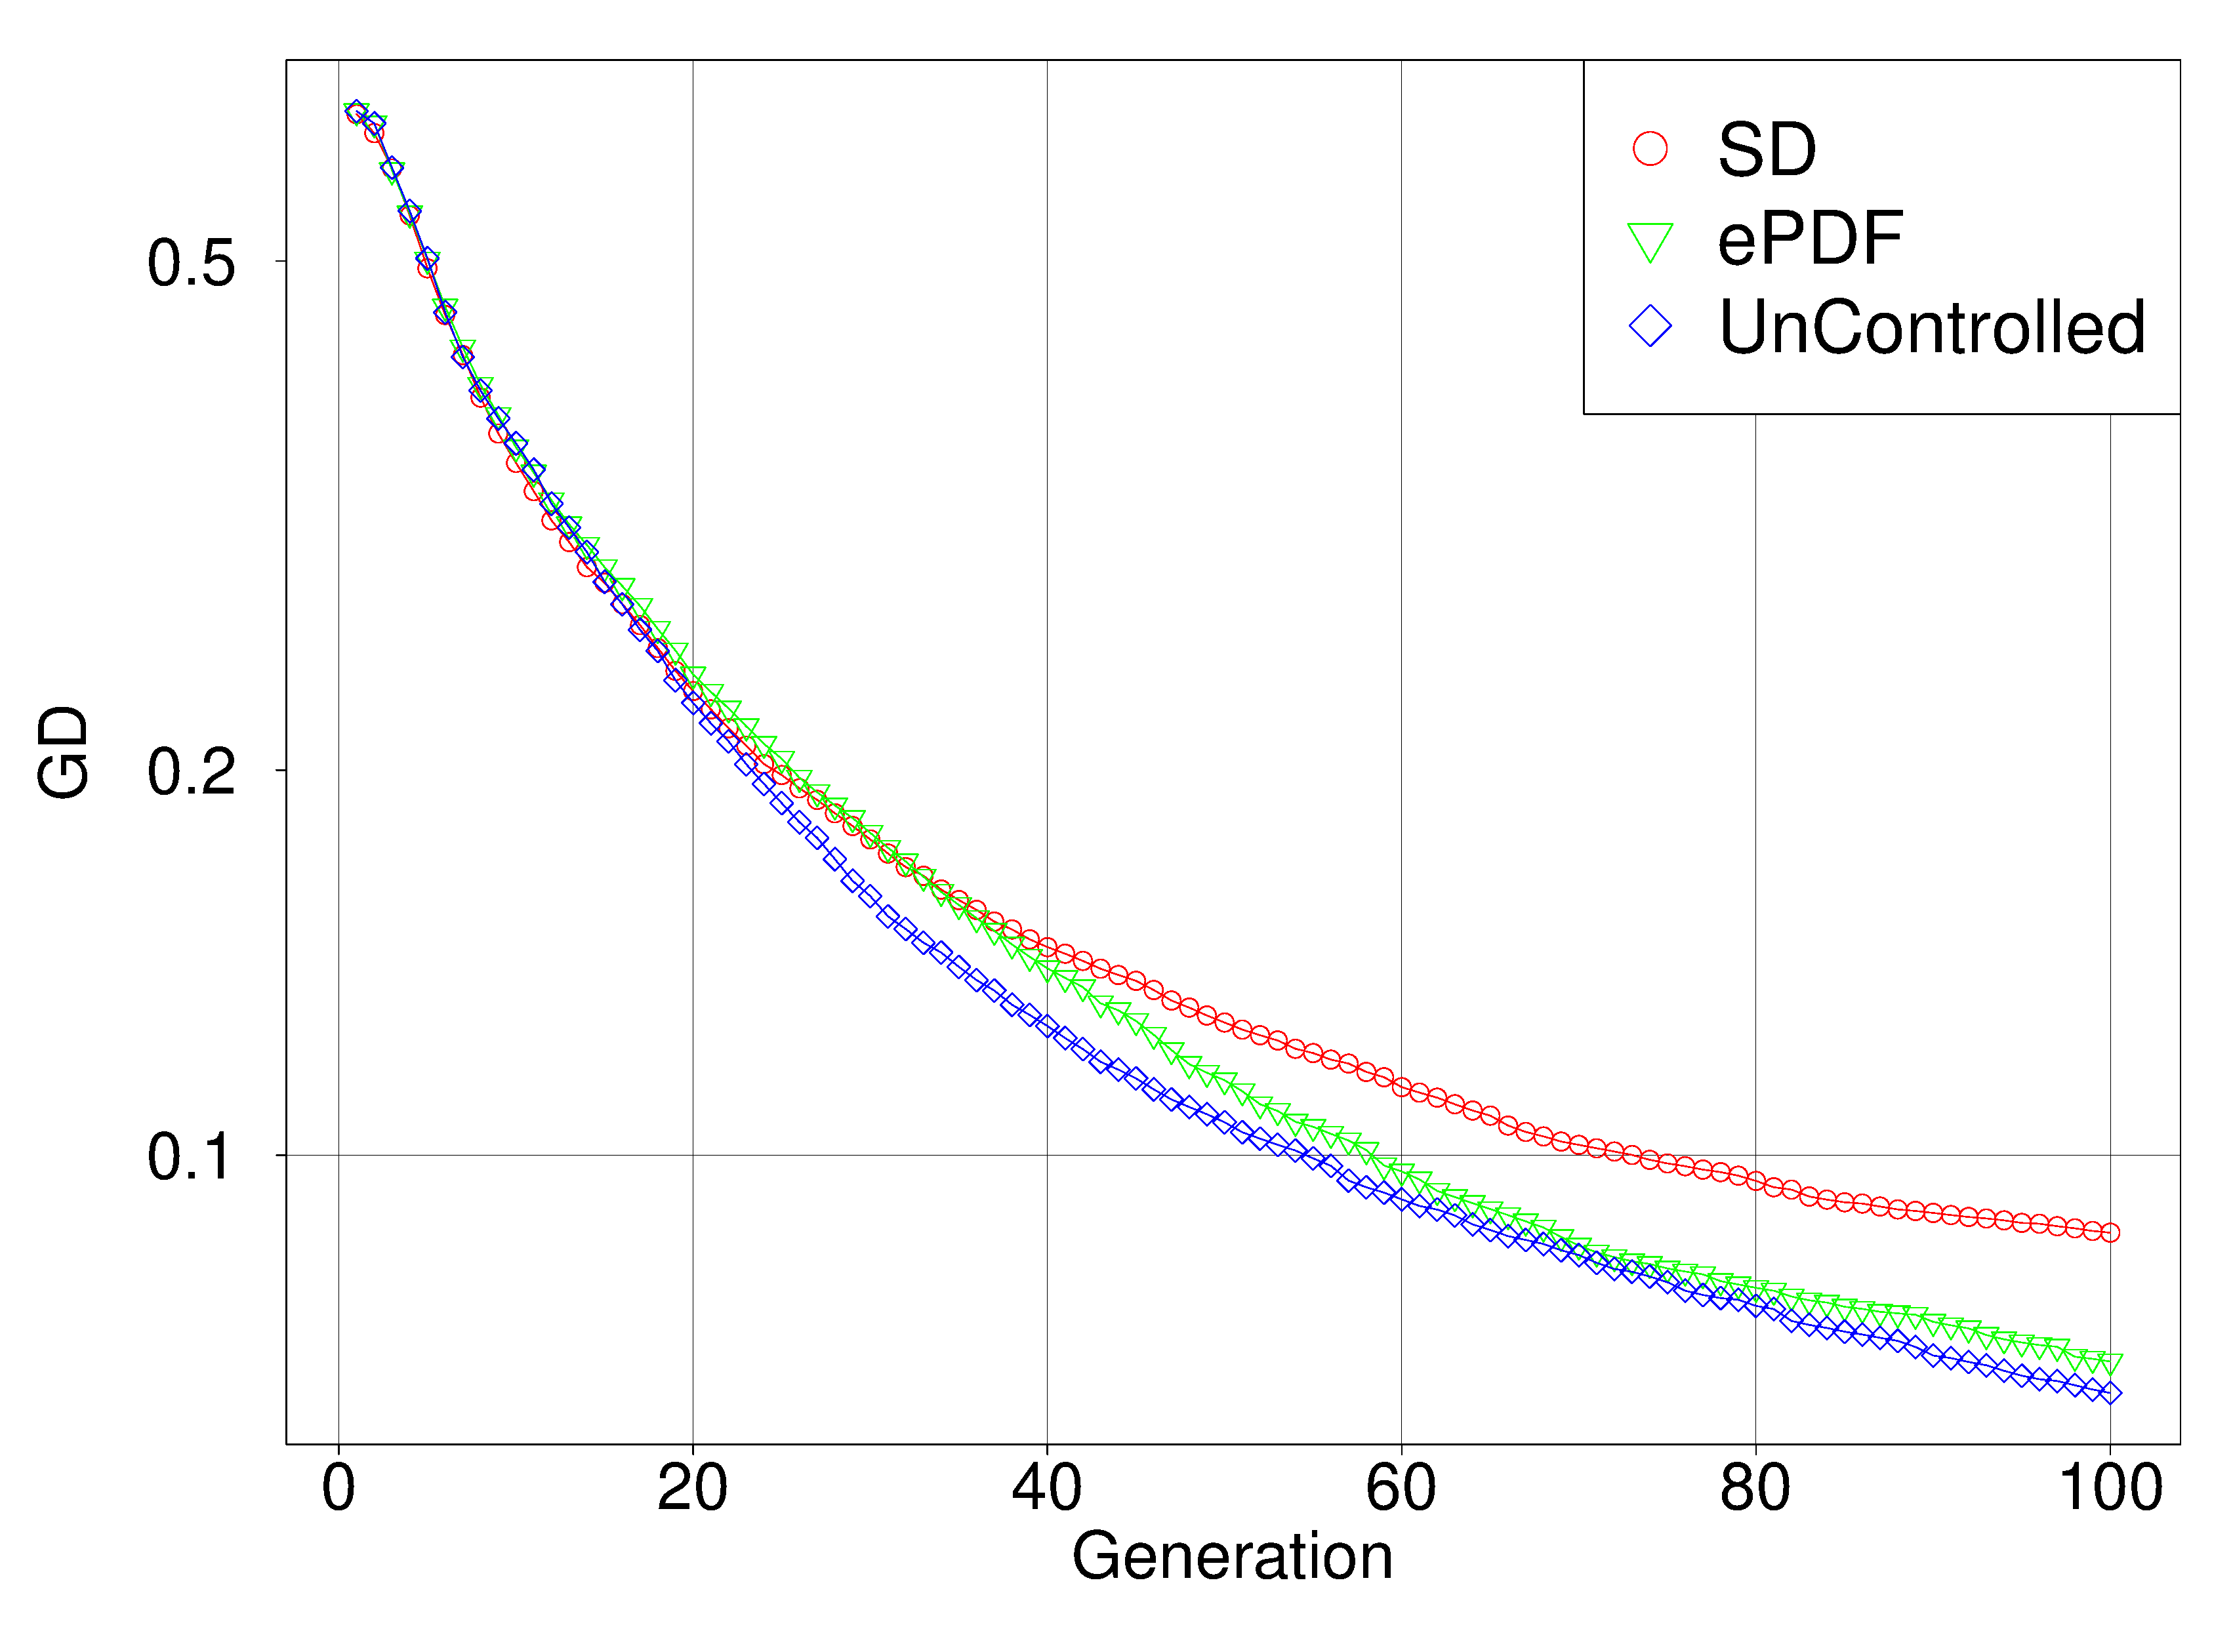
\includegraphics[width=1\linewidth]{../figures/WFG7_GD.eps}
\caption{適応的離散化手法を用いた場合と用いない場合のWFG7におけるGDの推移}
\label{wfg7_gd_transition}
\end{minipage}
\begin{minipage}{0.49\hsize}
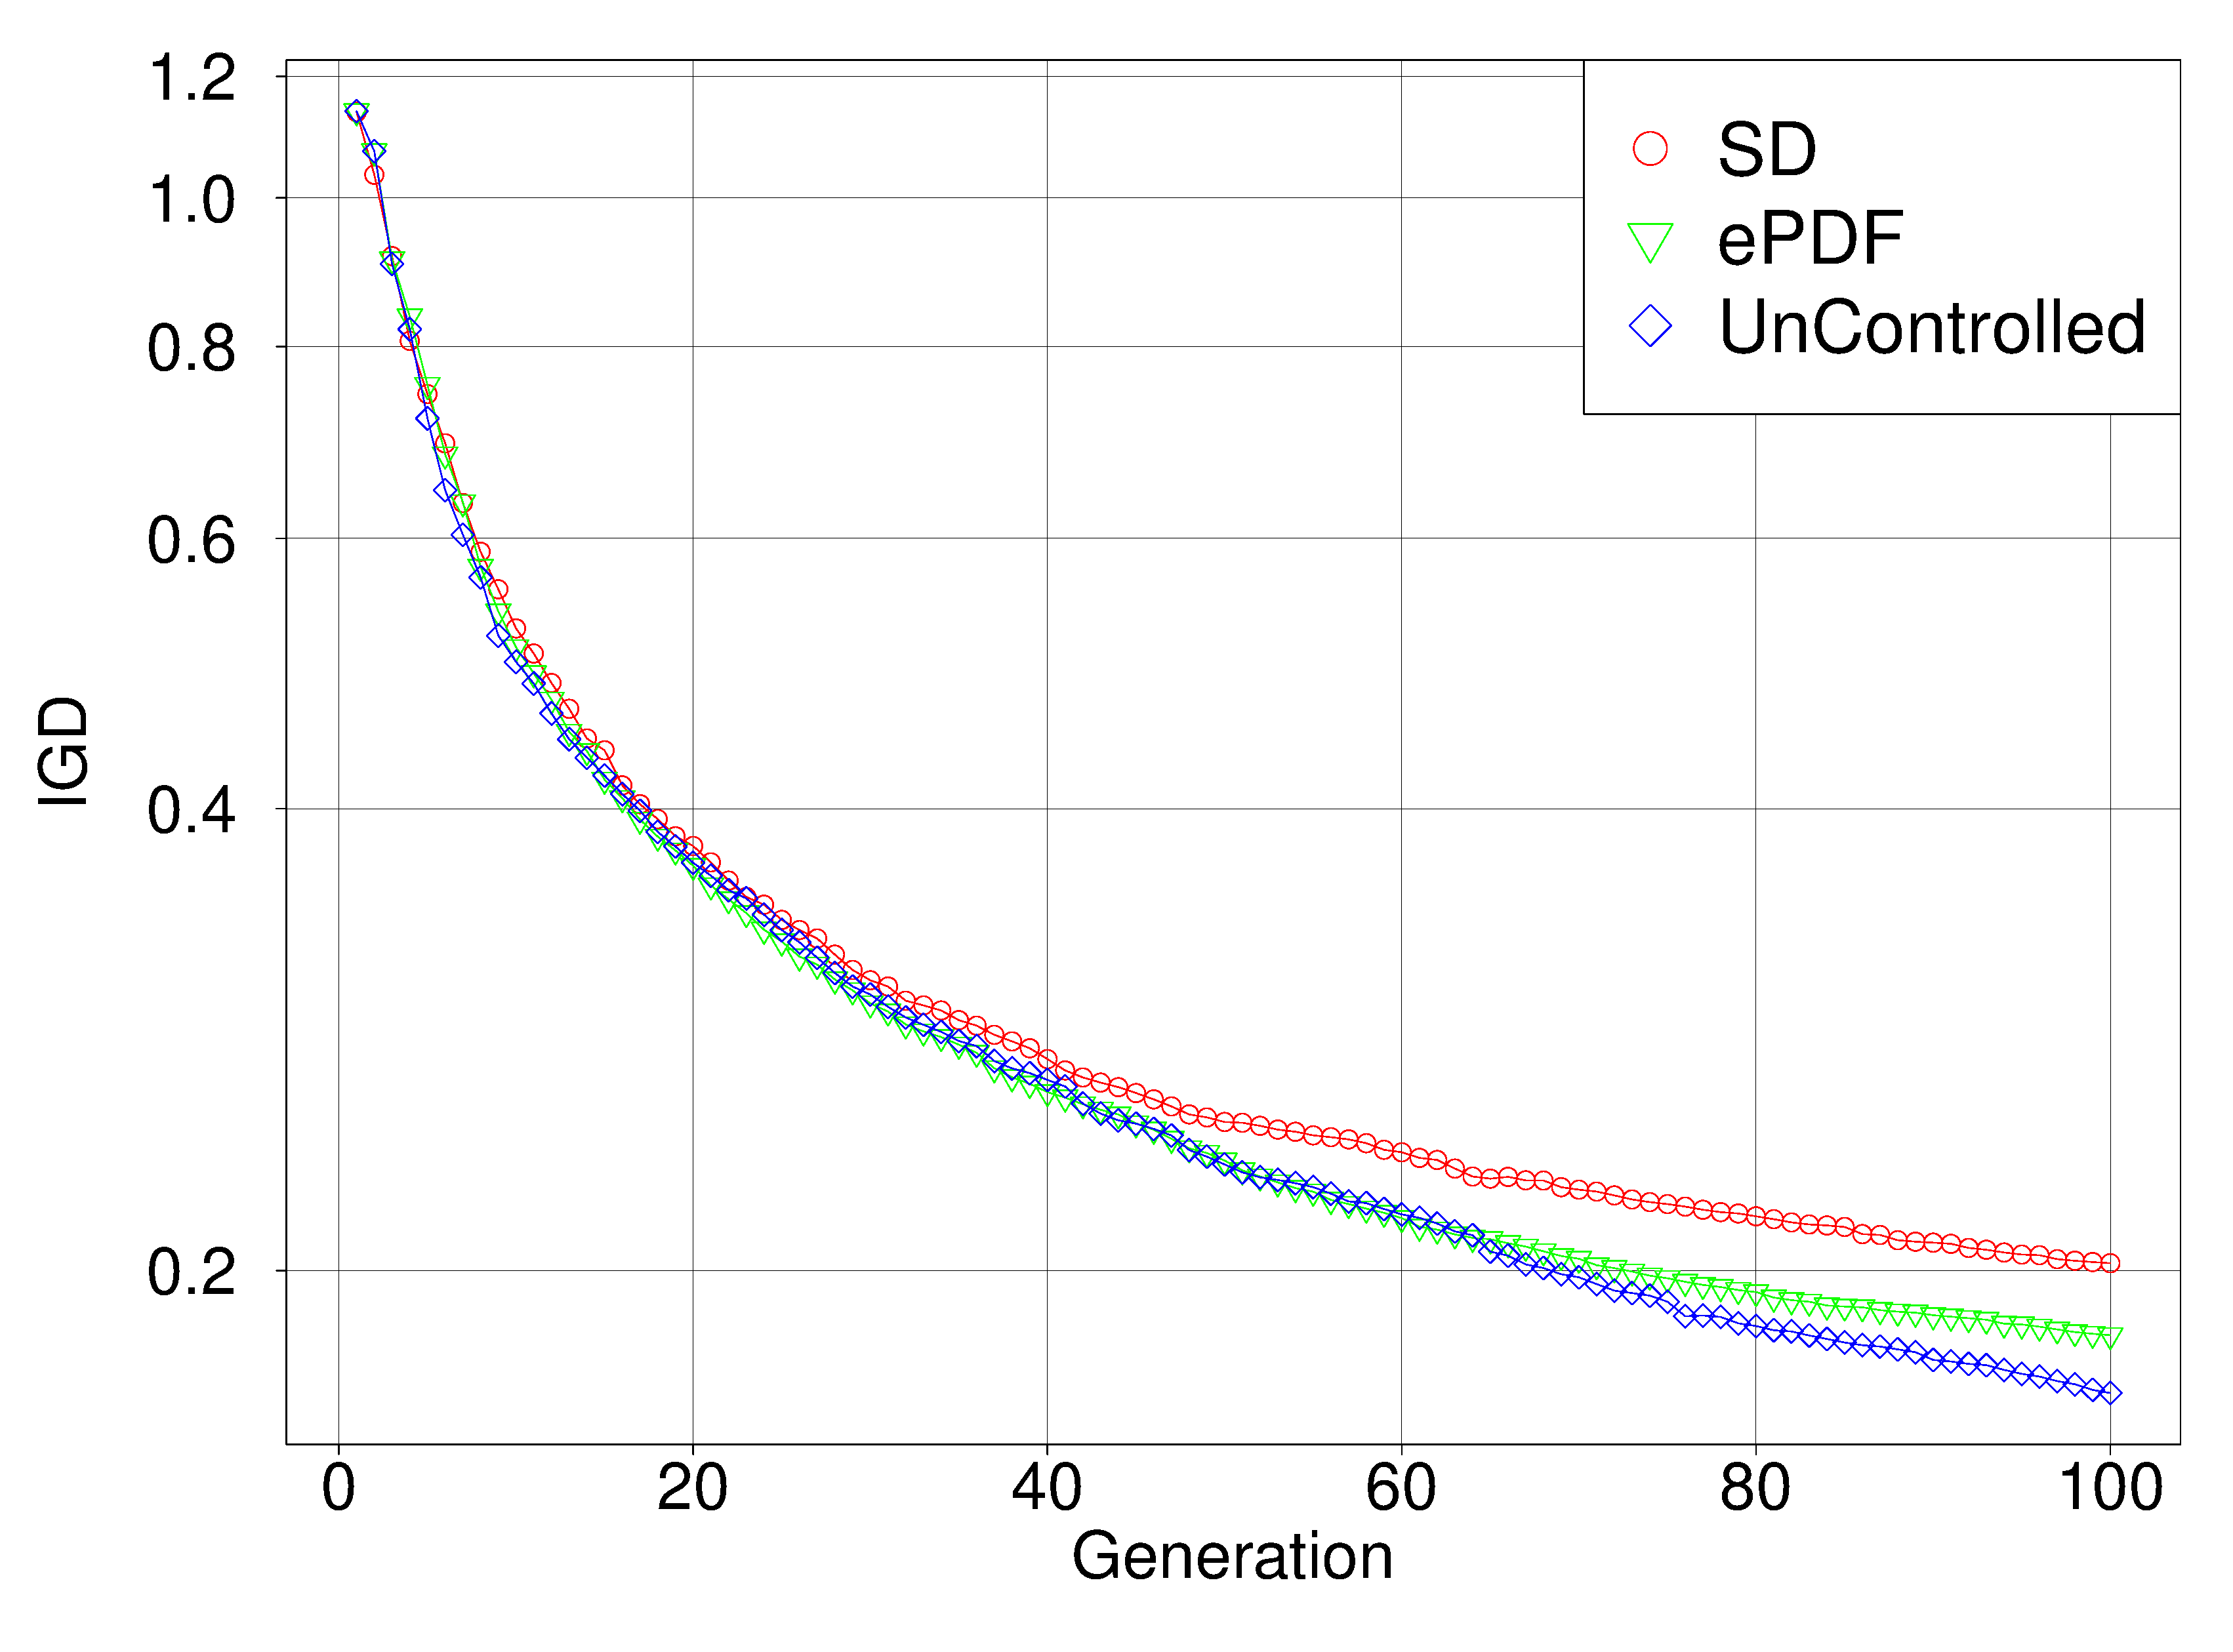
\includegraphics[width=1\linewidth]{../figures/WFG7_IGD.eps}
\caption{適応的離散化手法を用いた場合と用いない場合のWFG7におけるIGDの推移}
\label{wfg7_igd_transition}
\end{minipage}
\end{tabular}
\end{figure*}

\begin{figure*}[htbp]
\begin{tabular}{cc}
\begin{minipage}{0.33\hsize}
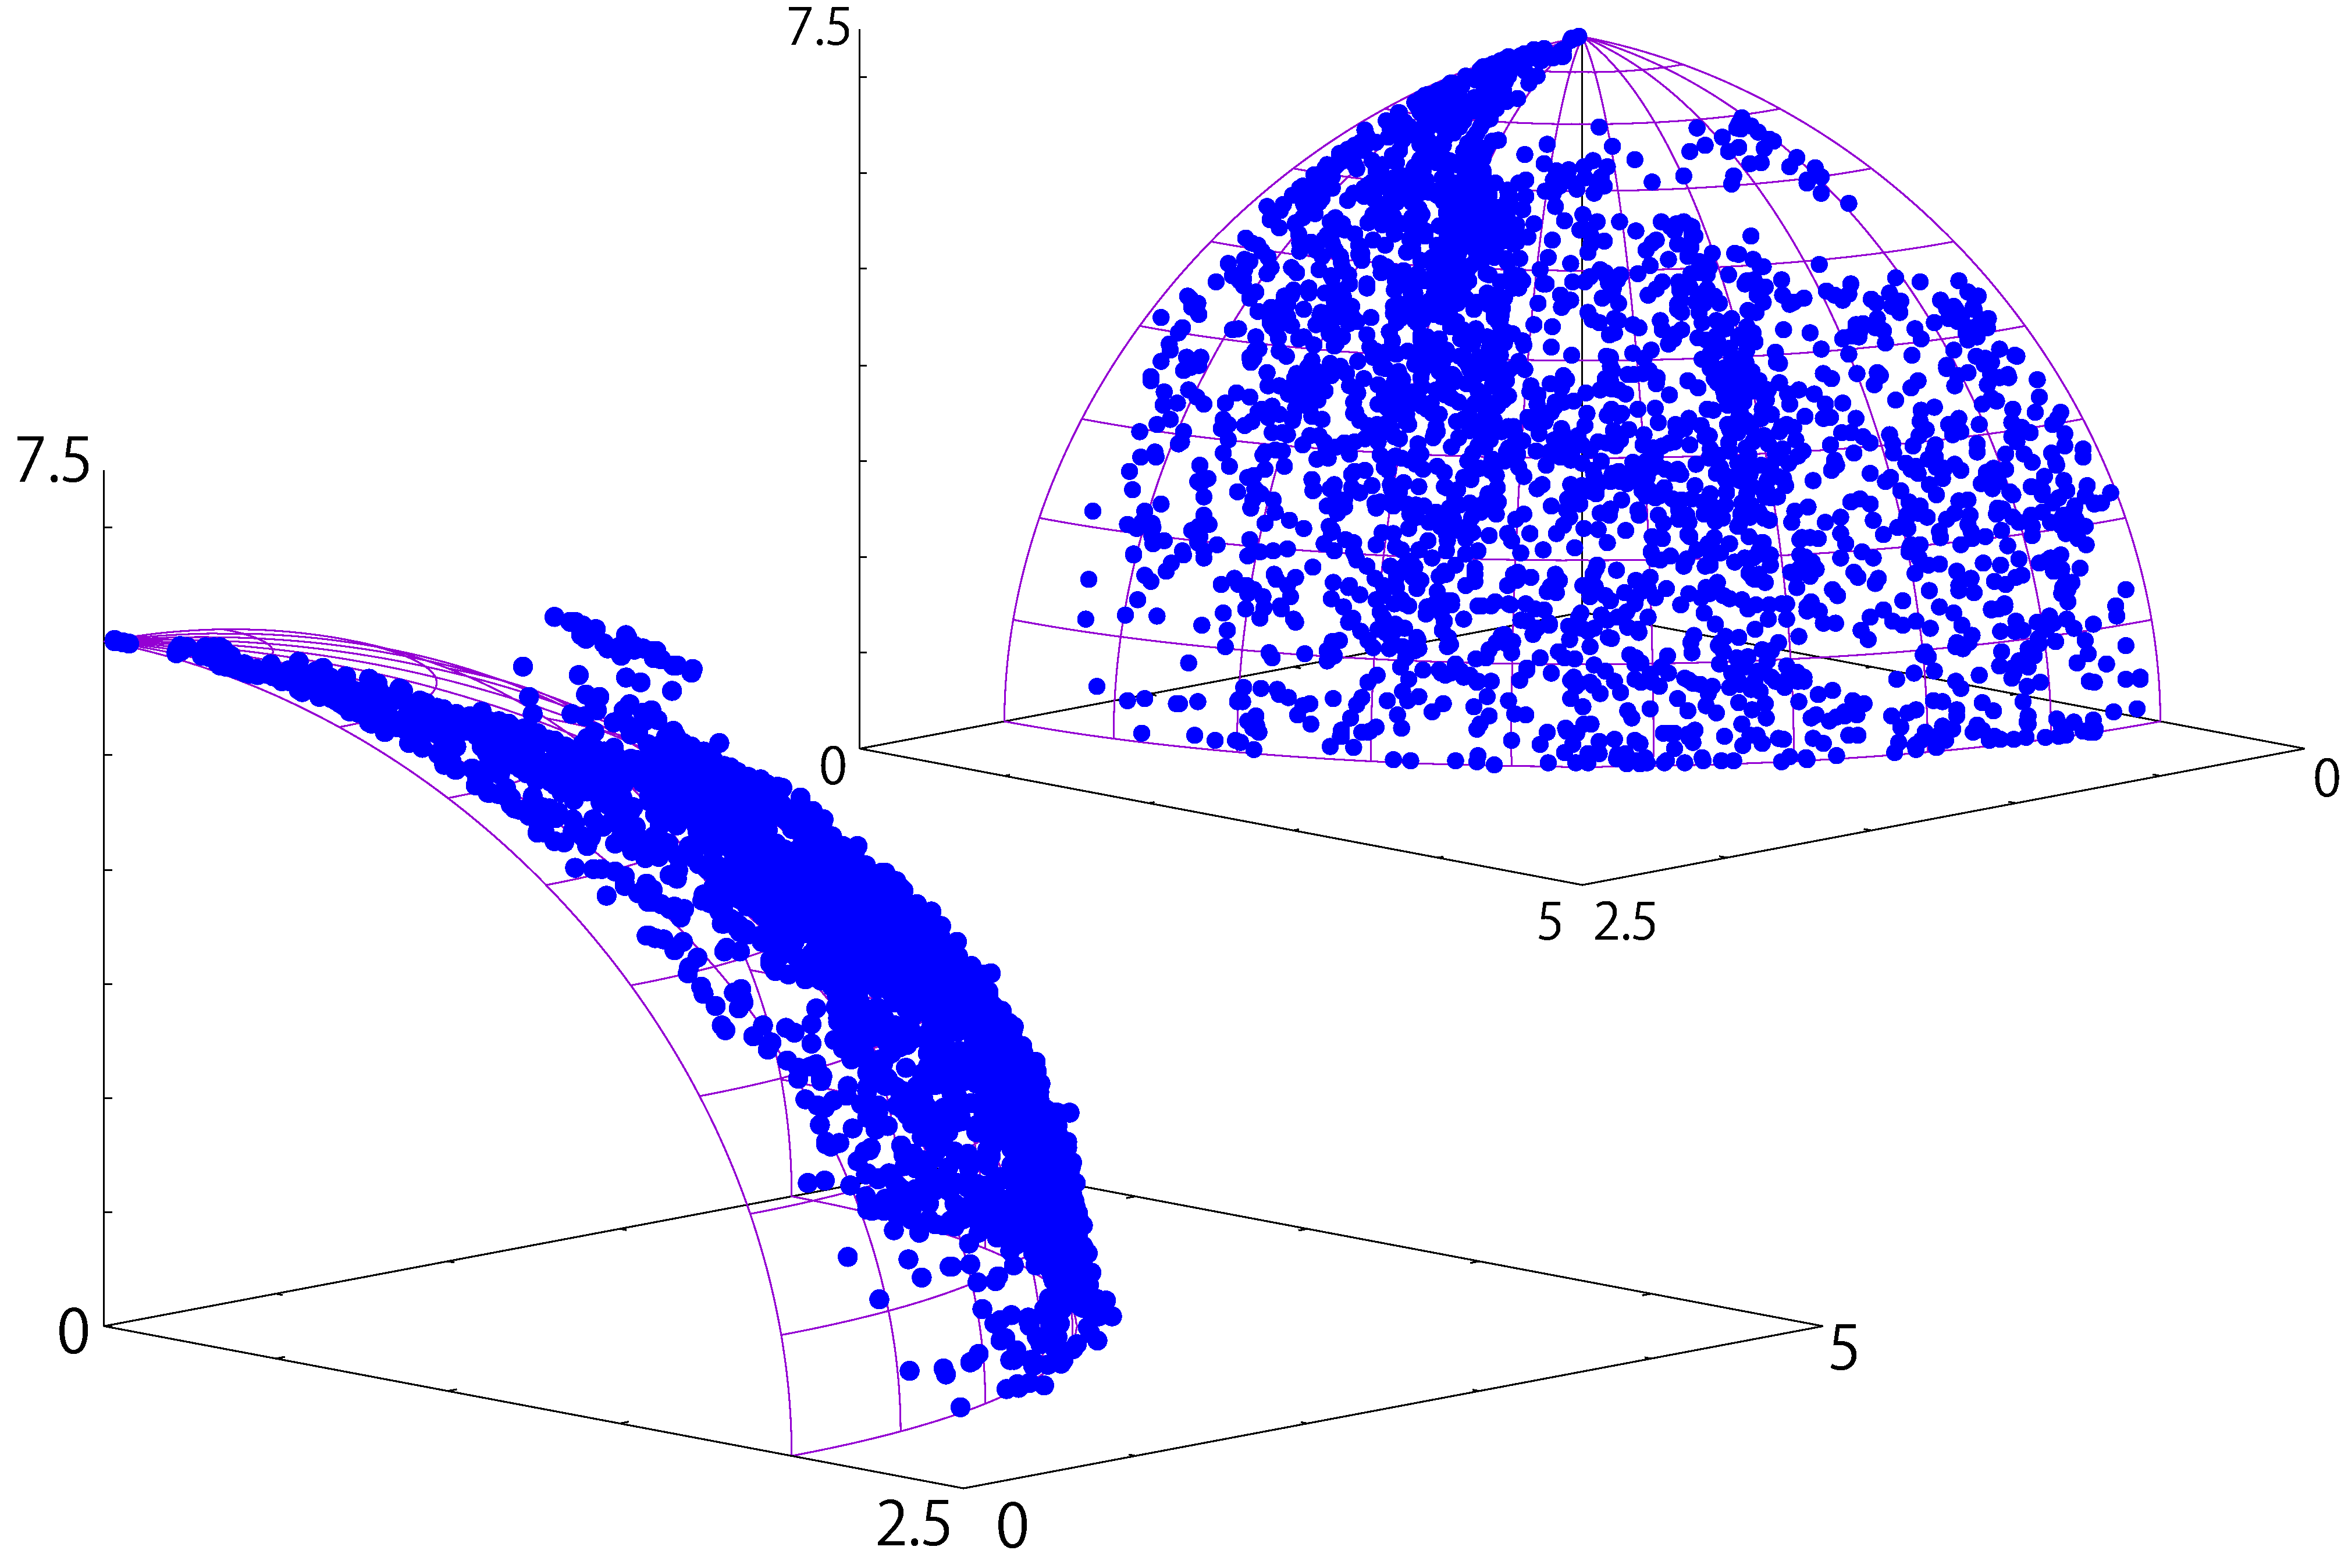
\includegraphics[width=1\linewidth]{../figures/WFG7_sd_double.pdf}
\begin{center}
{\footnotesize (a) SD}
\end{center}
\end{minipage}
\begin{minipage}{0.33\hsize}
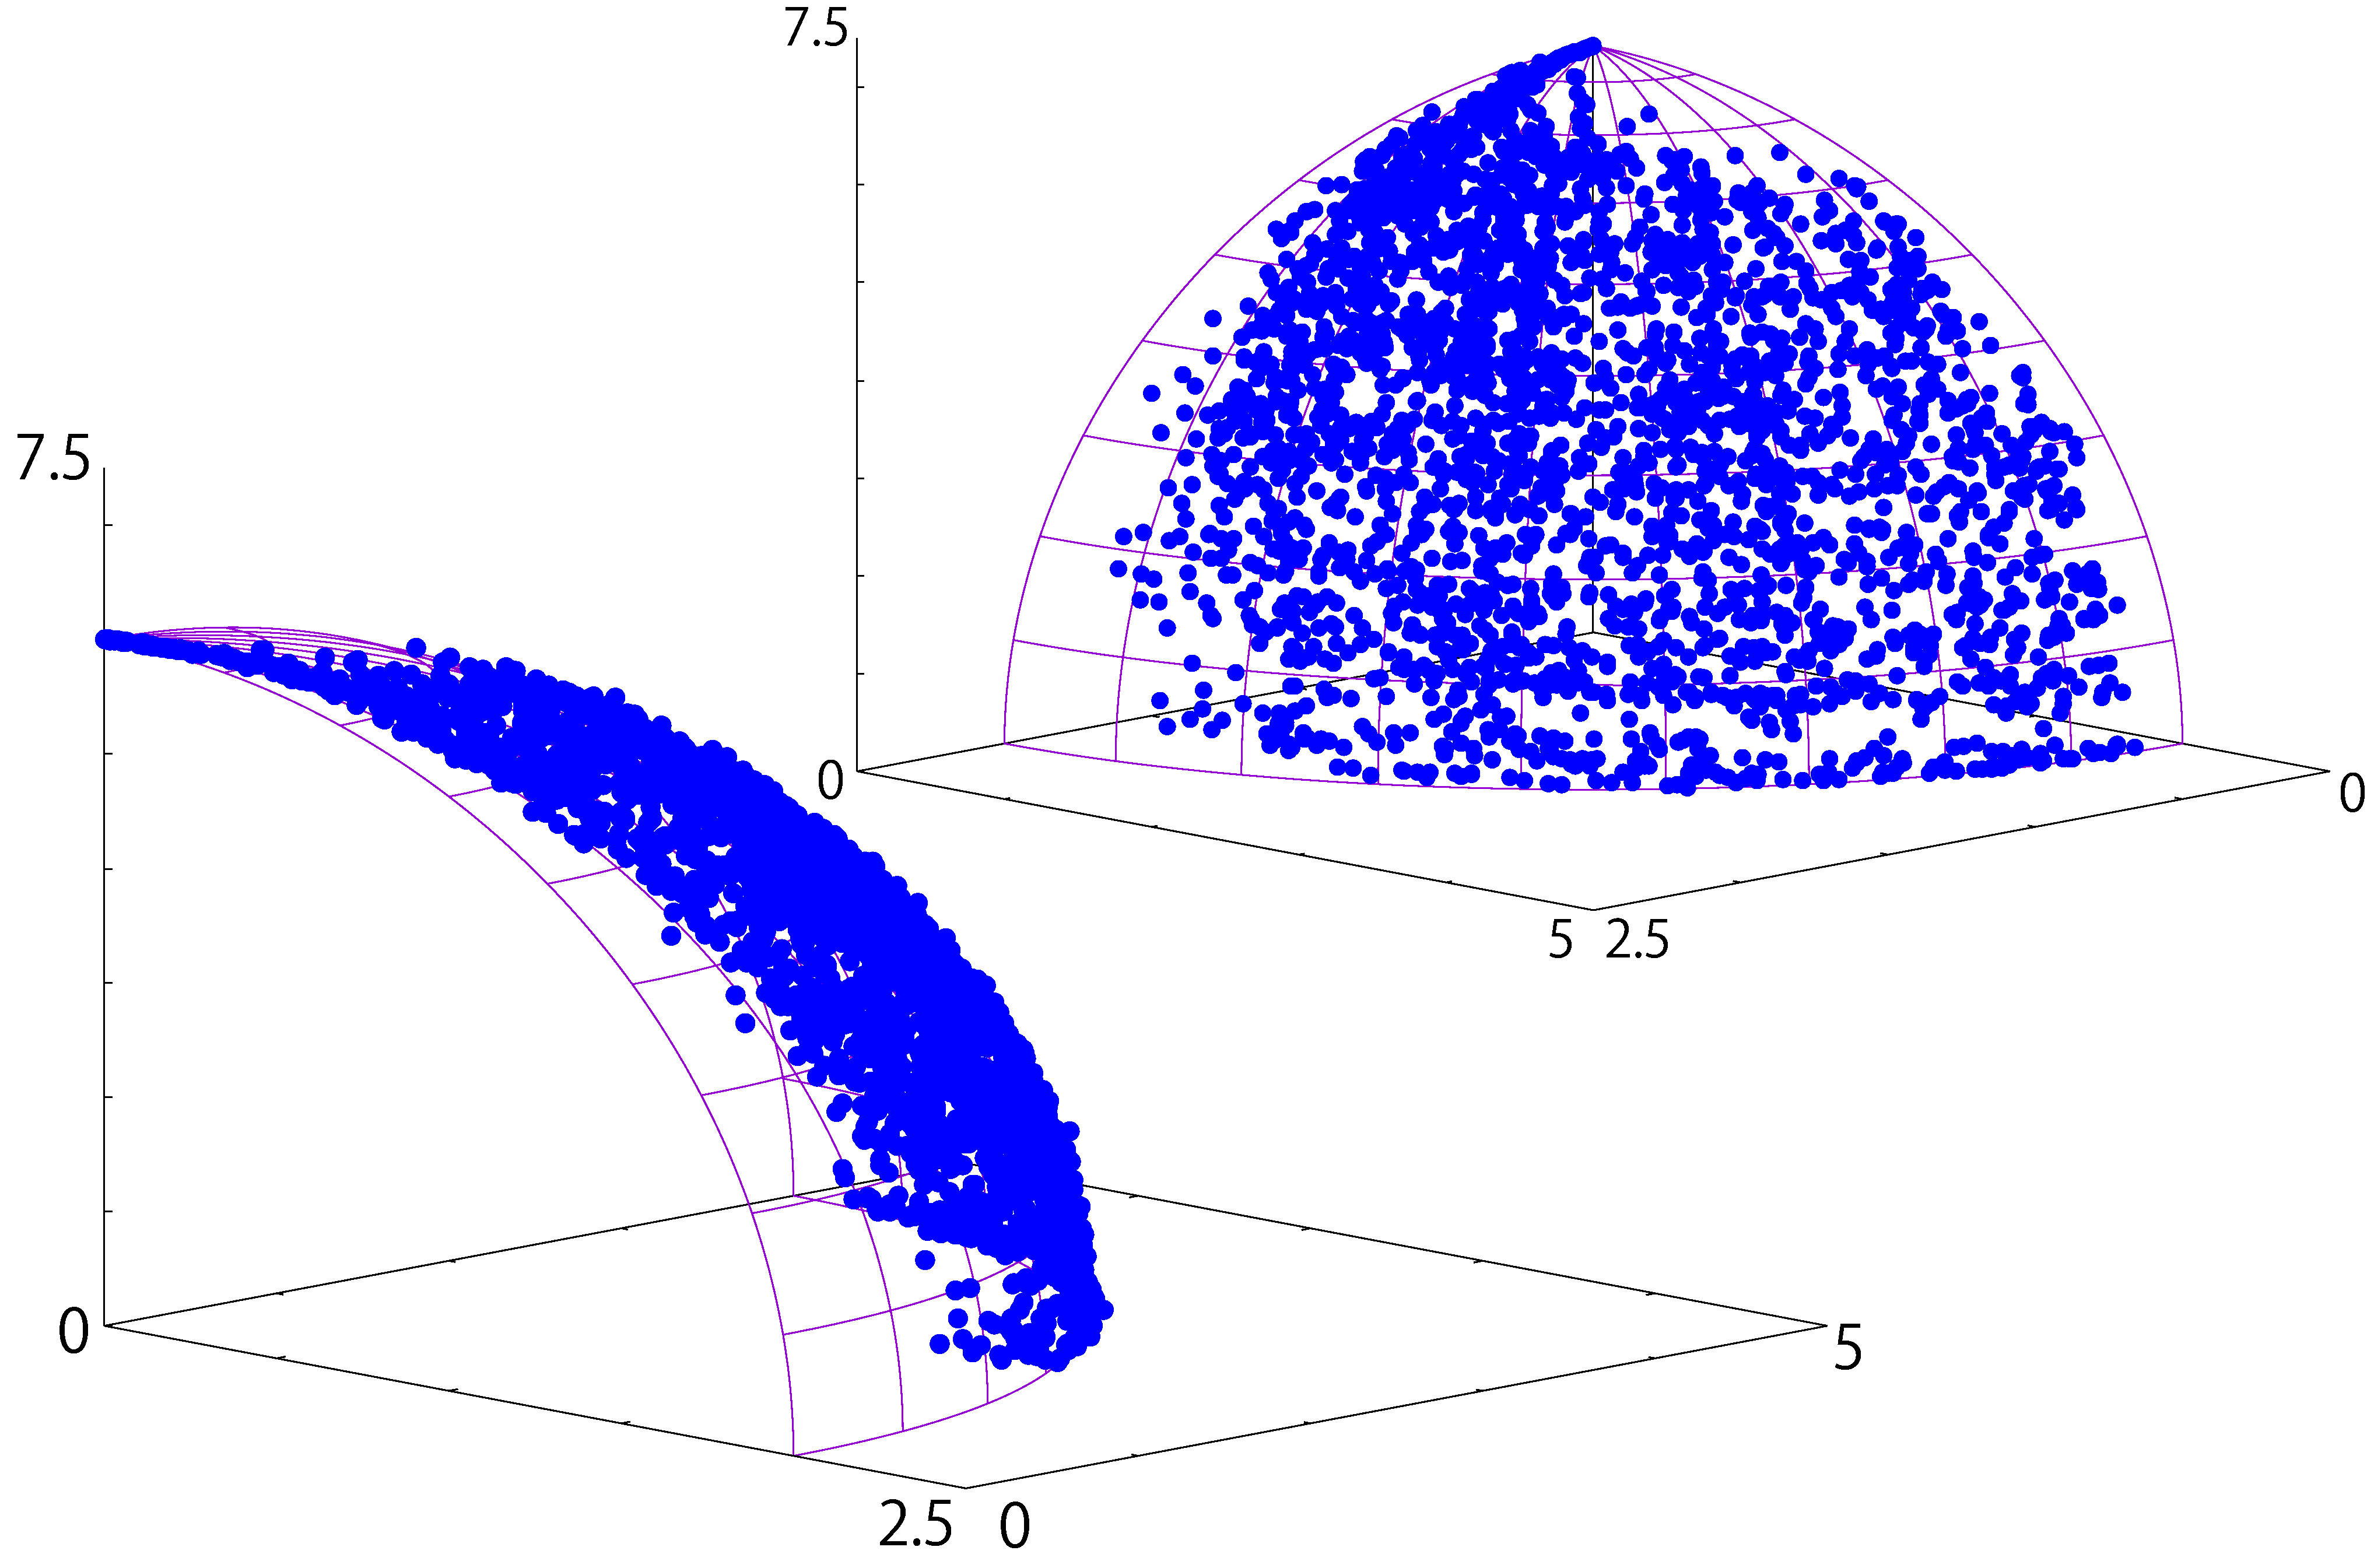
\includegraphics[width=1\linewidth]{../figures/WFG7_kde_double.pdf}
\begin{center}
{\footnotesize (b) ePDF}
\end{center}
\end{minipage}
\begin{minipage}{0.33\hsize}
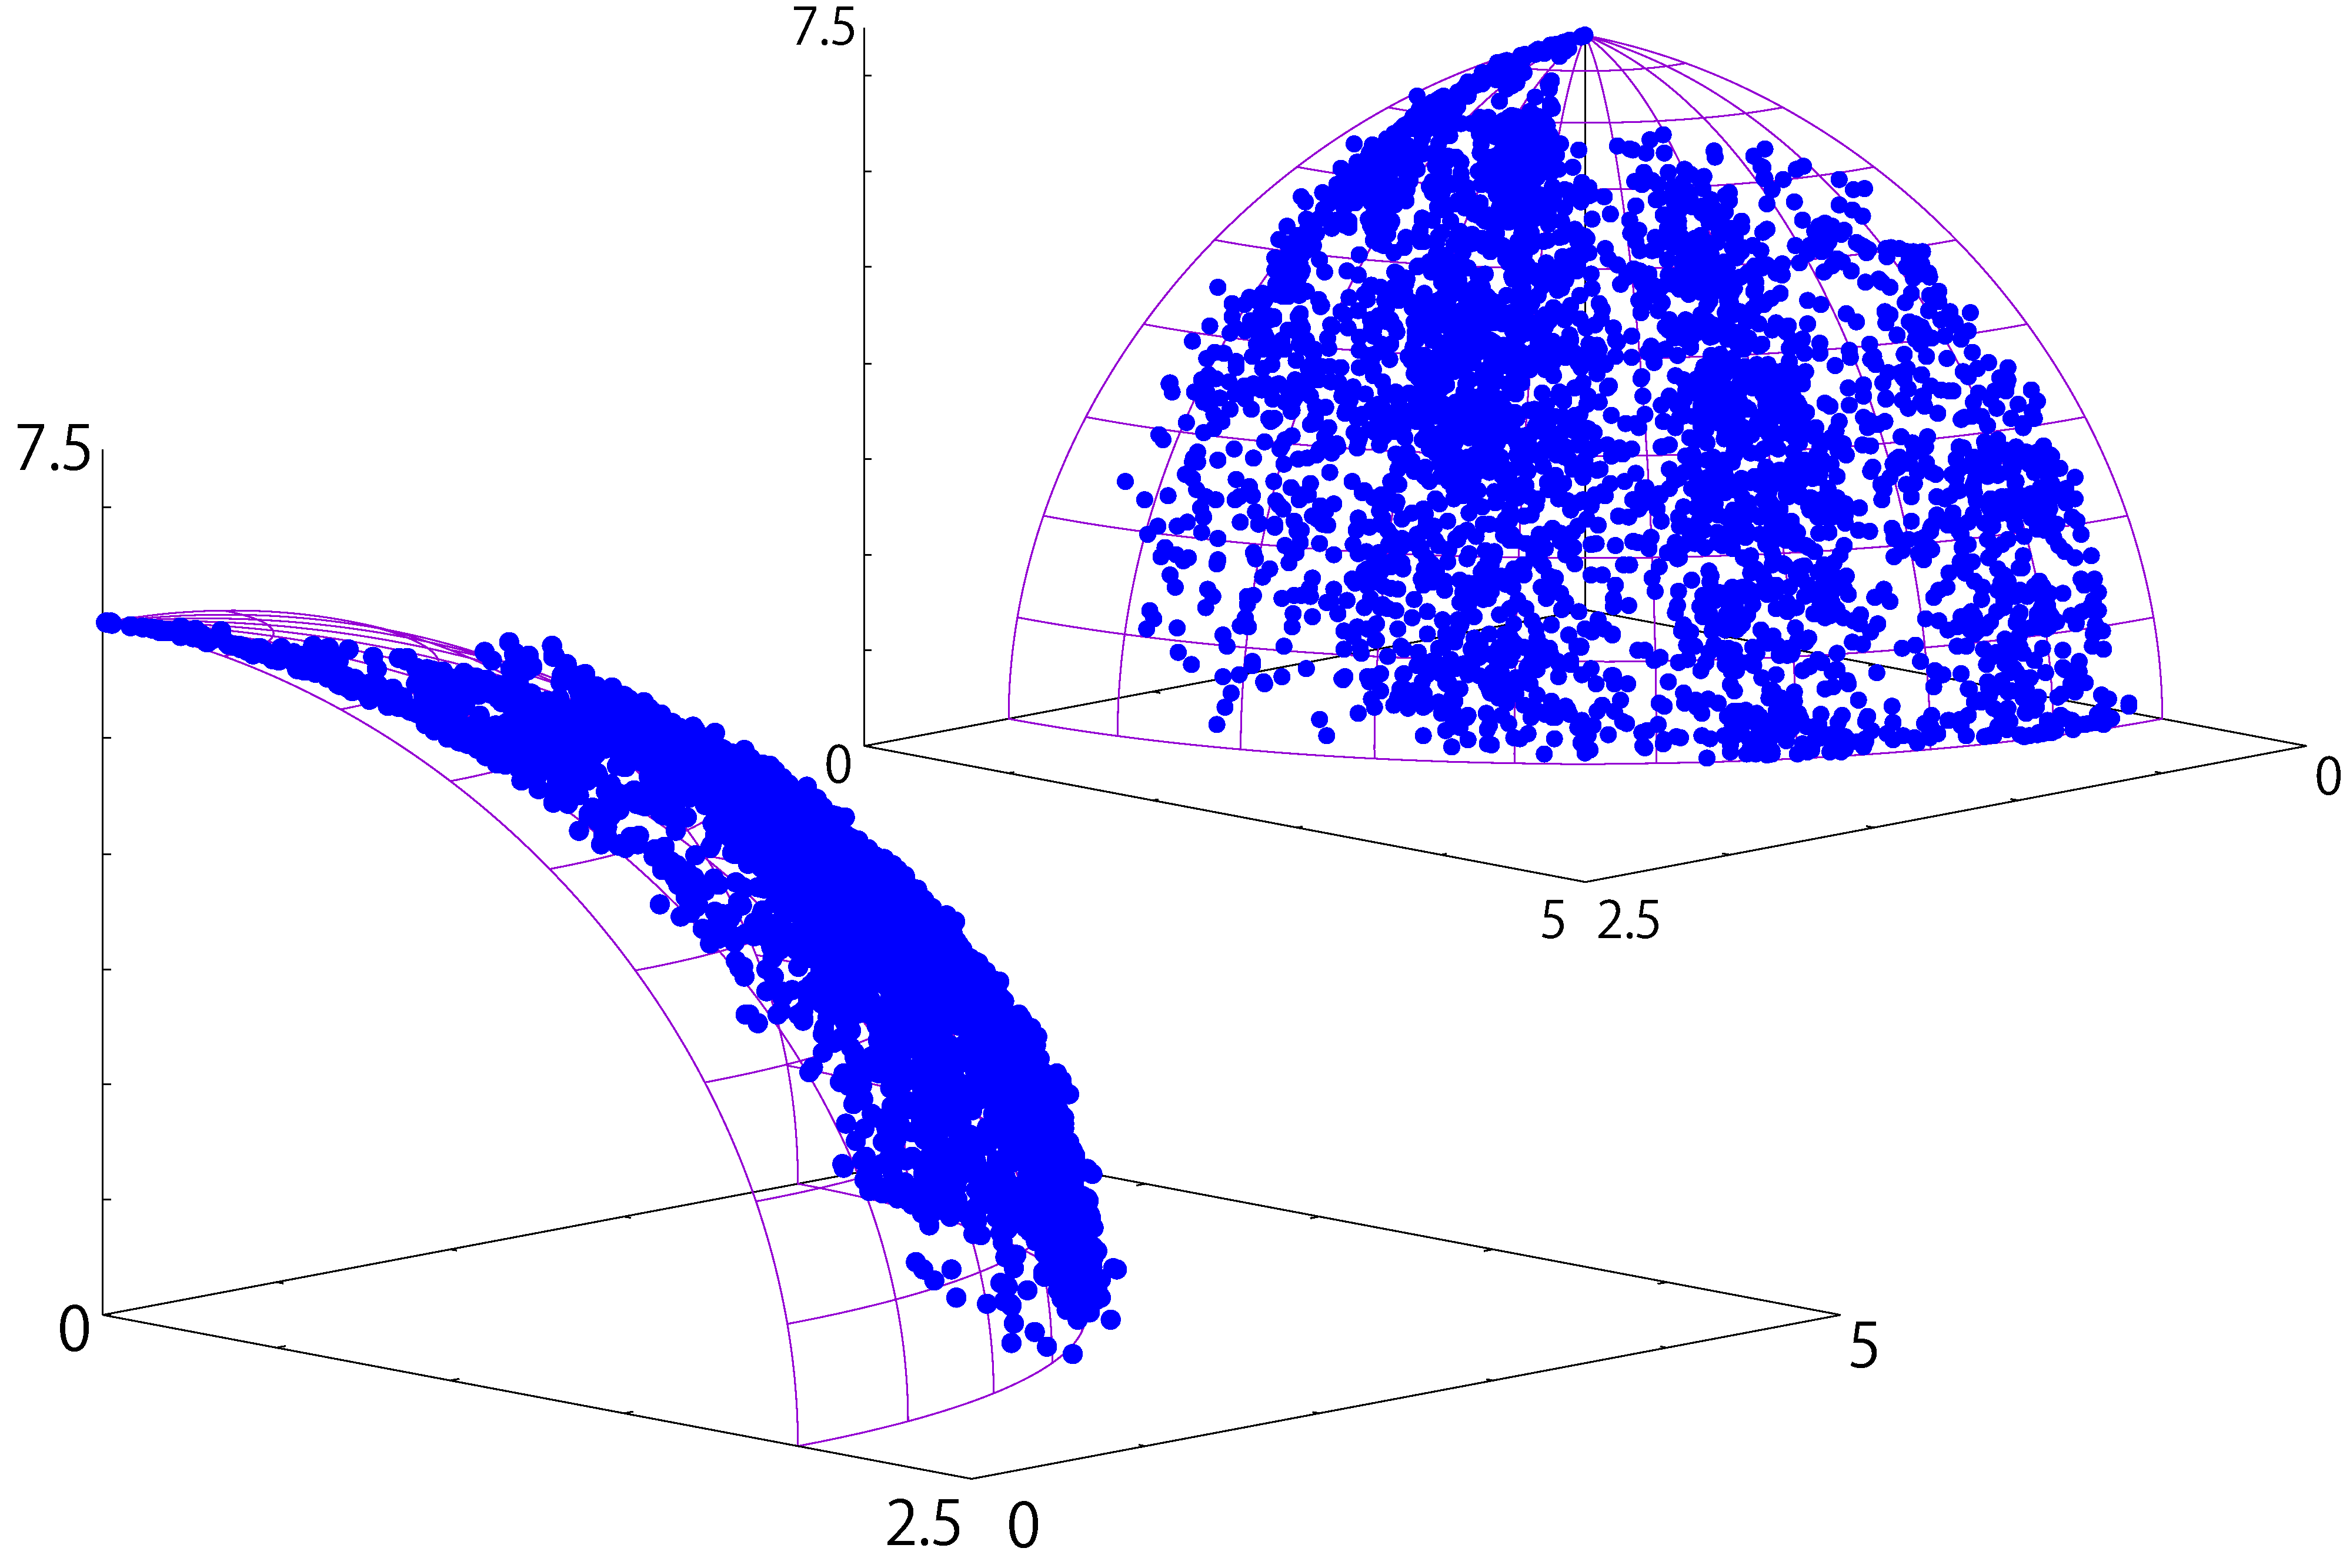
\includegraphics[width=1\linewidth]{../figures/WFG7_uc_double.pdf}
\begin{center}
{\footnotesize (c) 制御なし}
\end{center}
\end{minipage}
\end{tabular}
\caption{適応的離散化手法を用いた場合と用いない場合のWFG7におけるGDの推移}
\label{fig:nondoms_wfg7}
\end{figure*}

\begin{figure*}[!h]
\begin{minipage}{0.38\hsize}
\vspace{-0.2in}
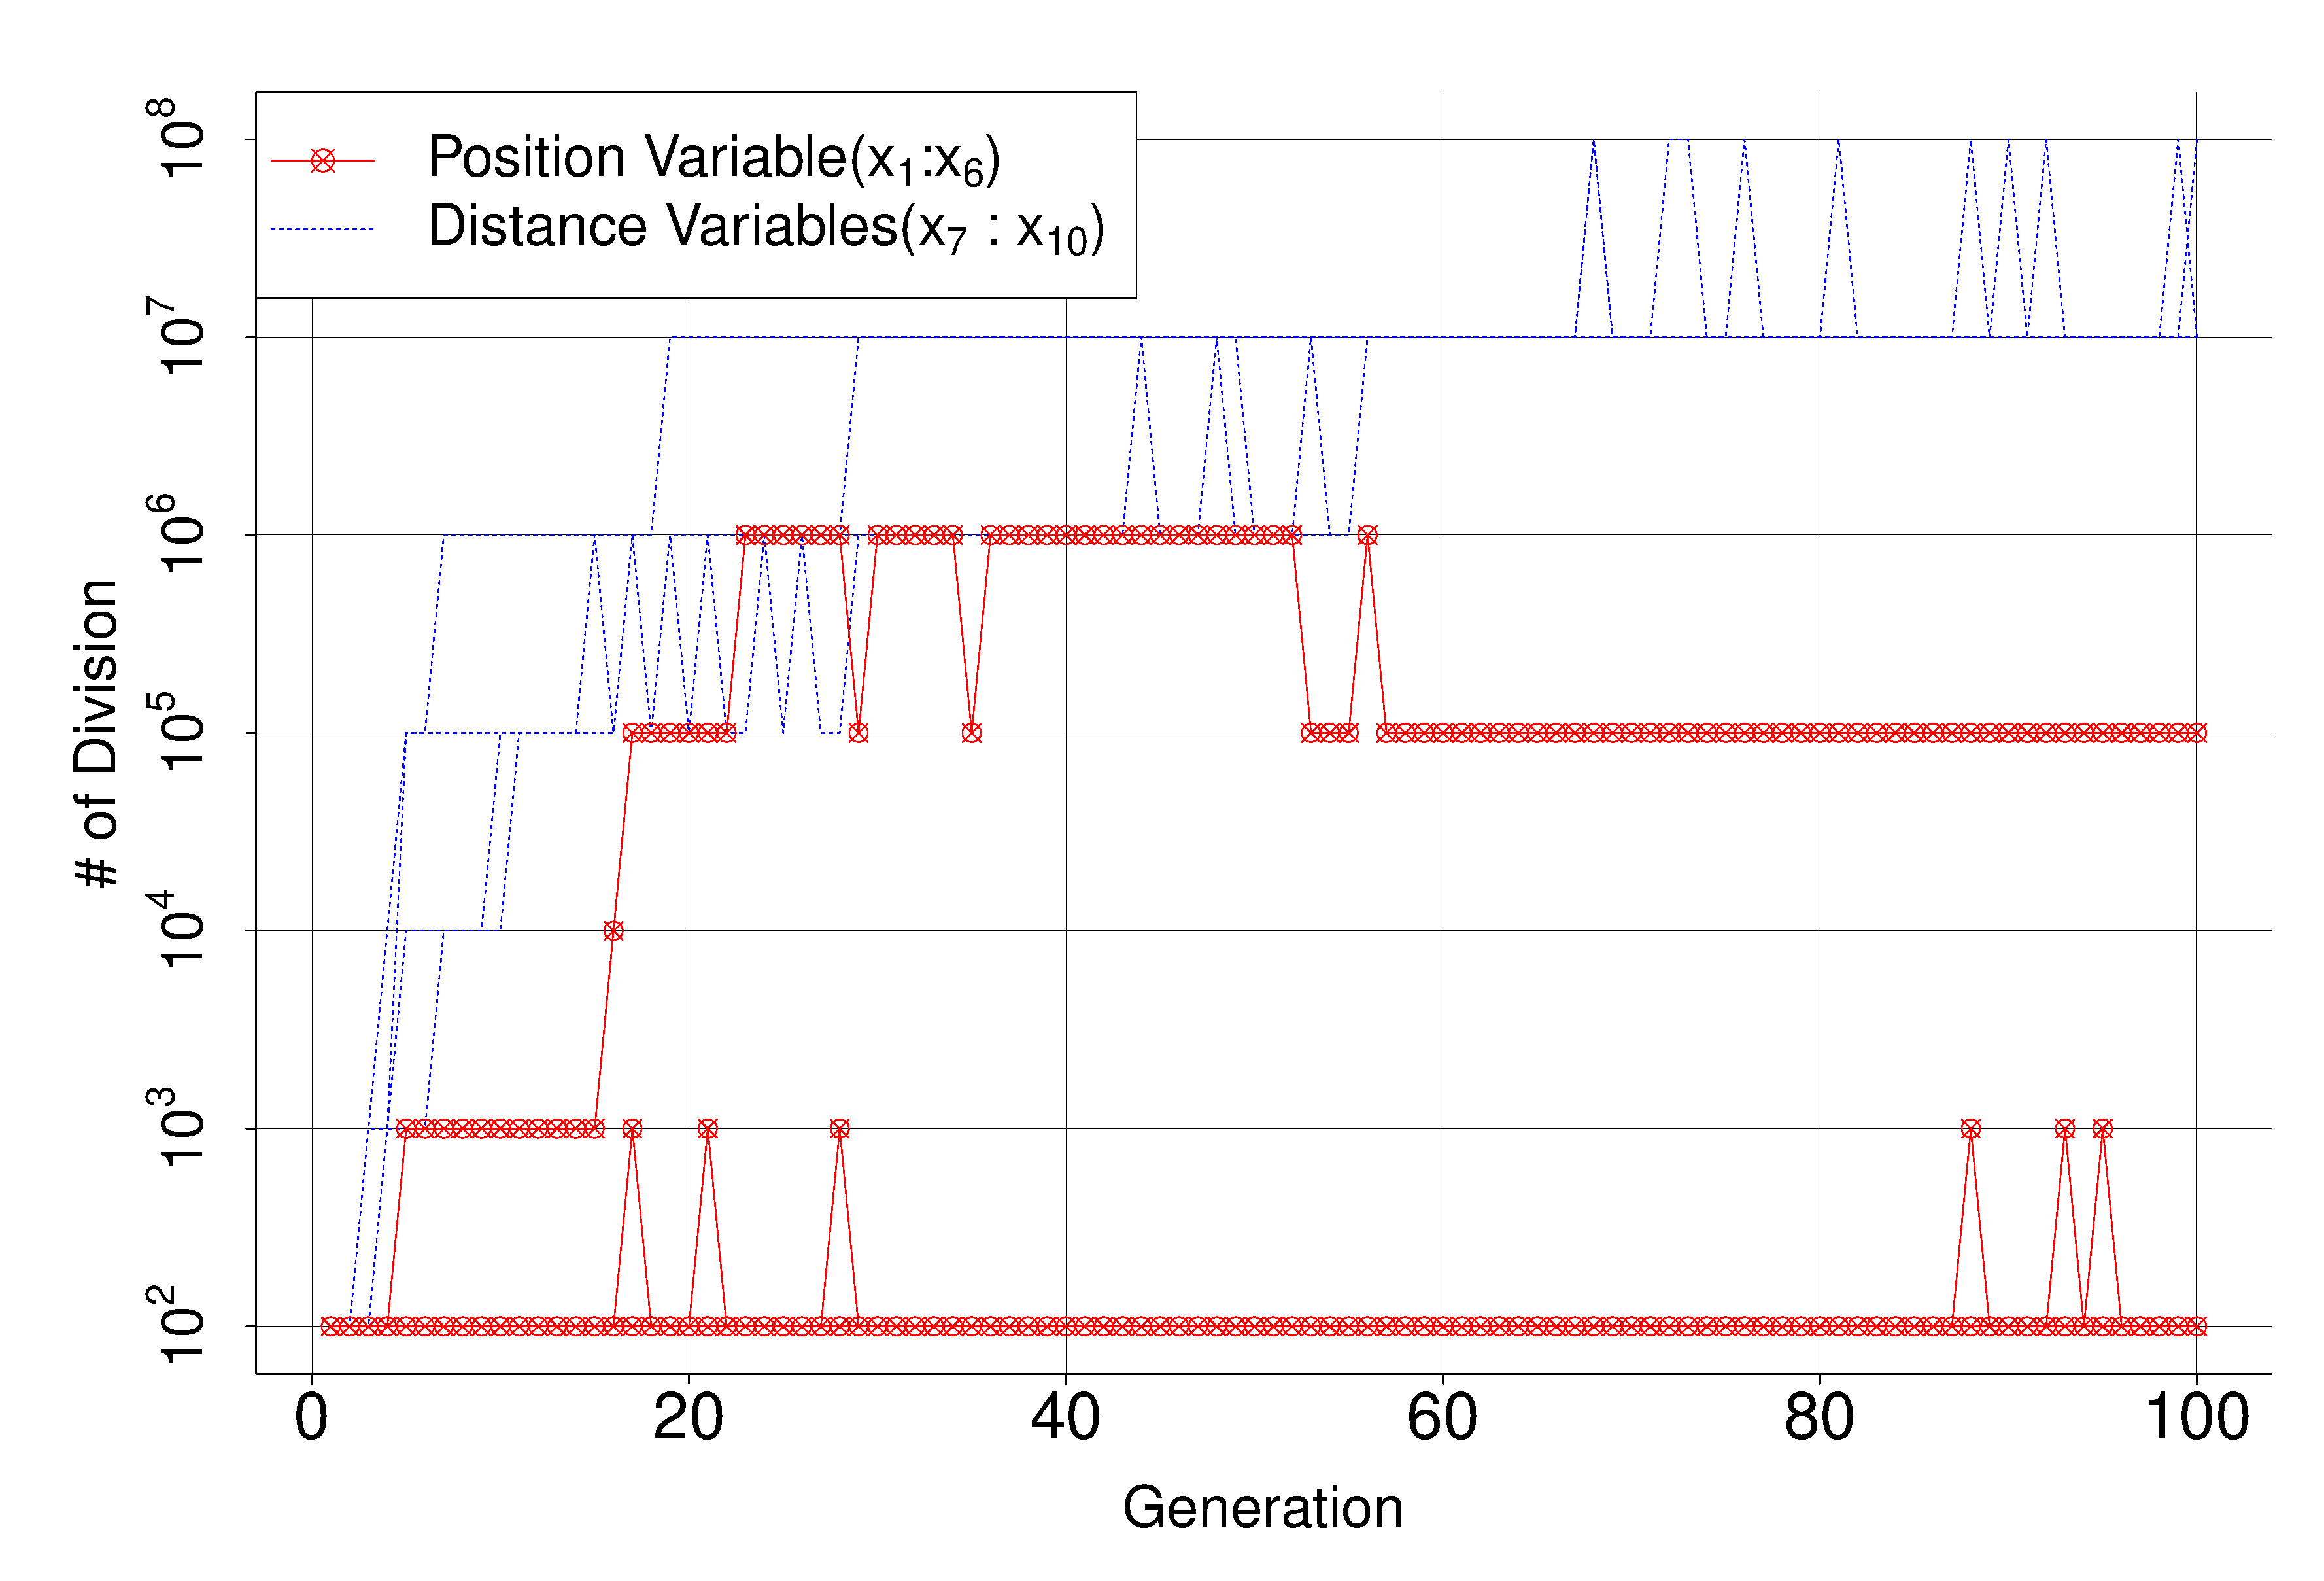
\includegraphics[width=1\linewidth]{../figures/WFG7_digit_trend.eps}\\
\\
\caption{SDを用いた場合のWFG7における各設計変数の分割数の世代ごとの推移}
\label{digi_trans_wfg7}
\end{minipage}
\begin{minipage}{0.61\hsize}
\begin{minipage}{0.49\hsize}
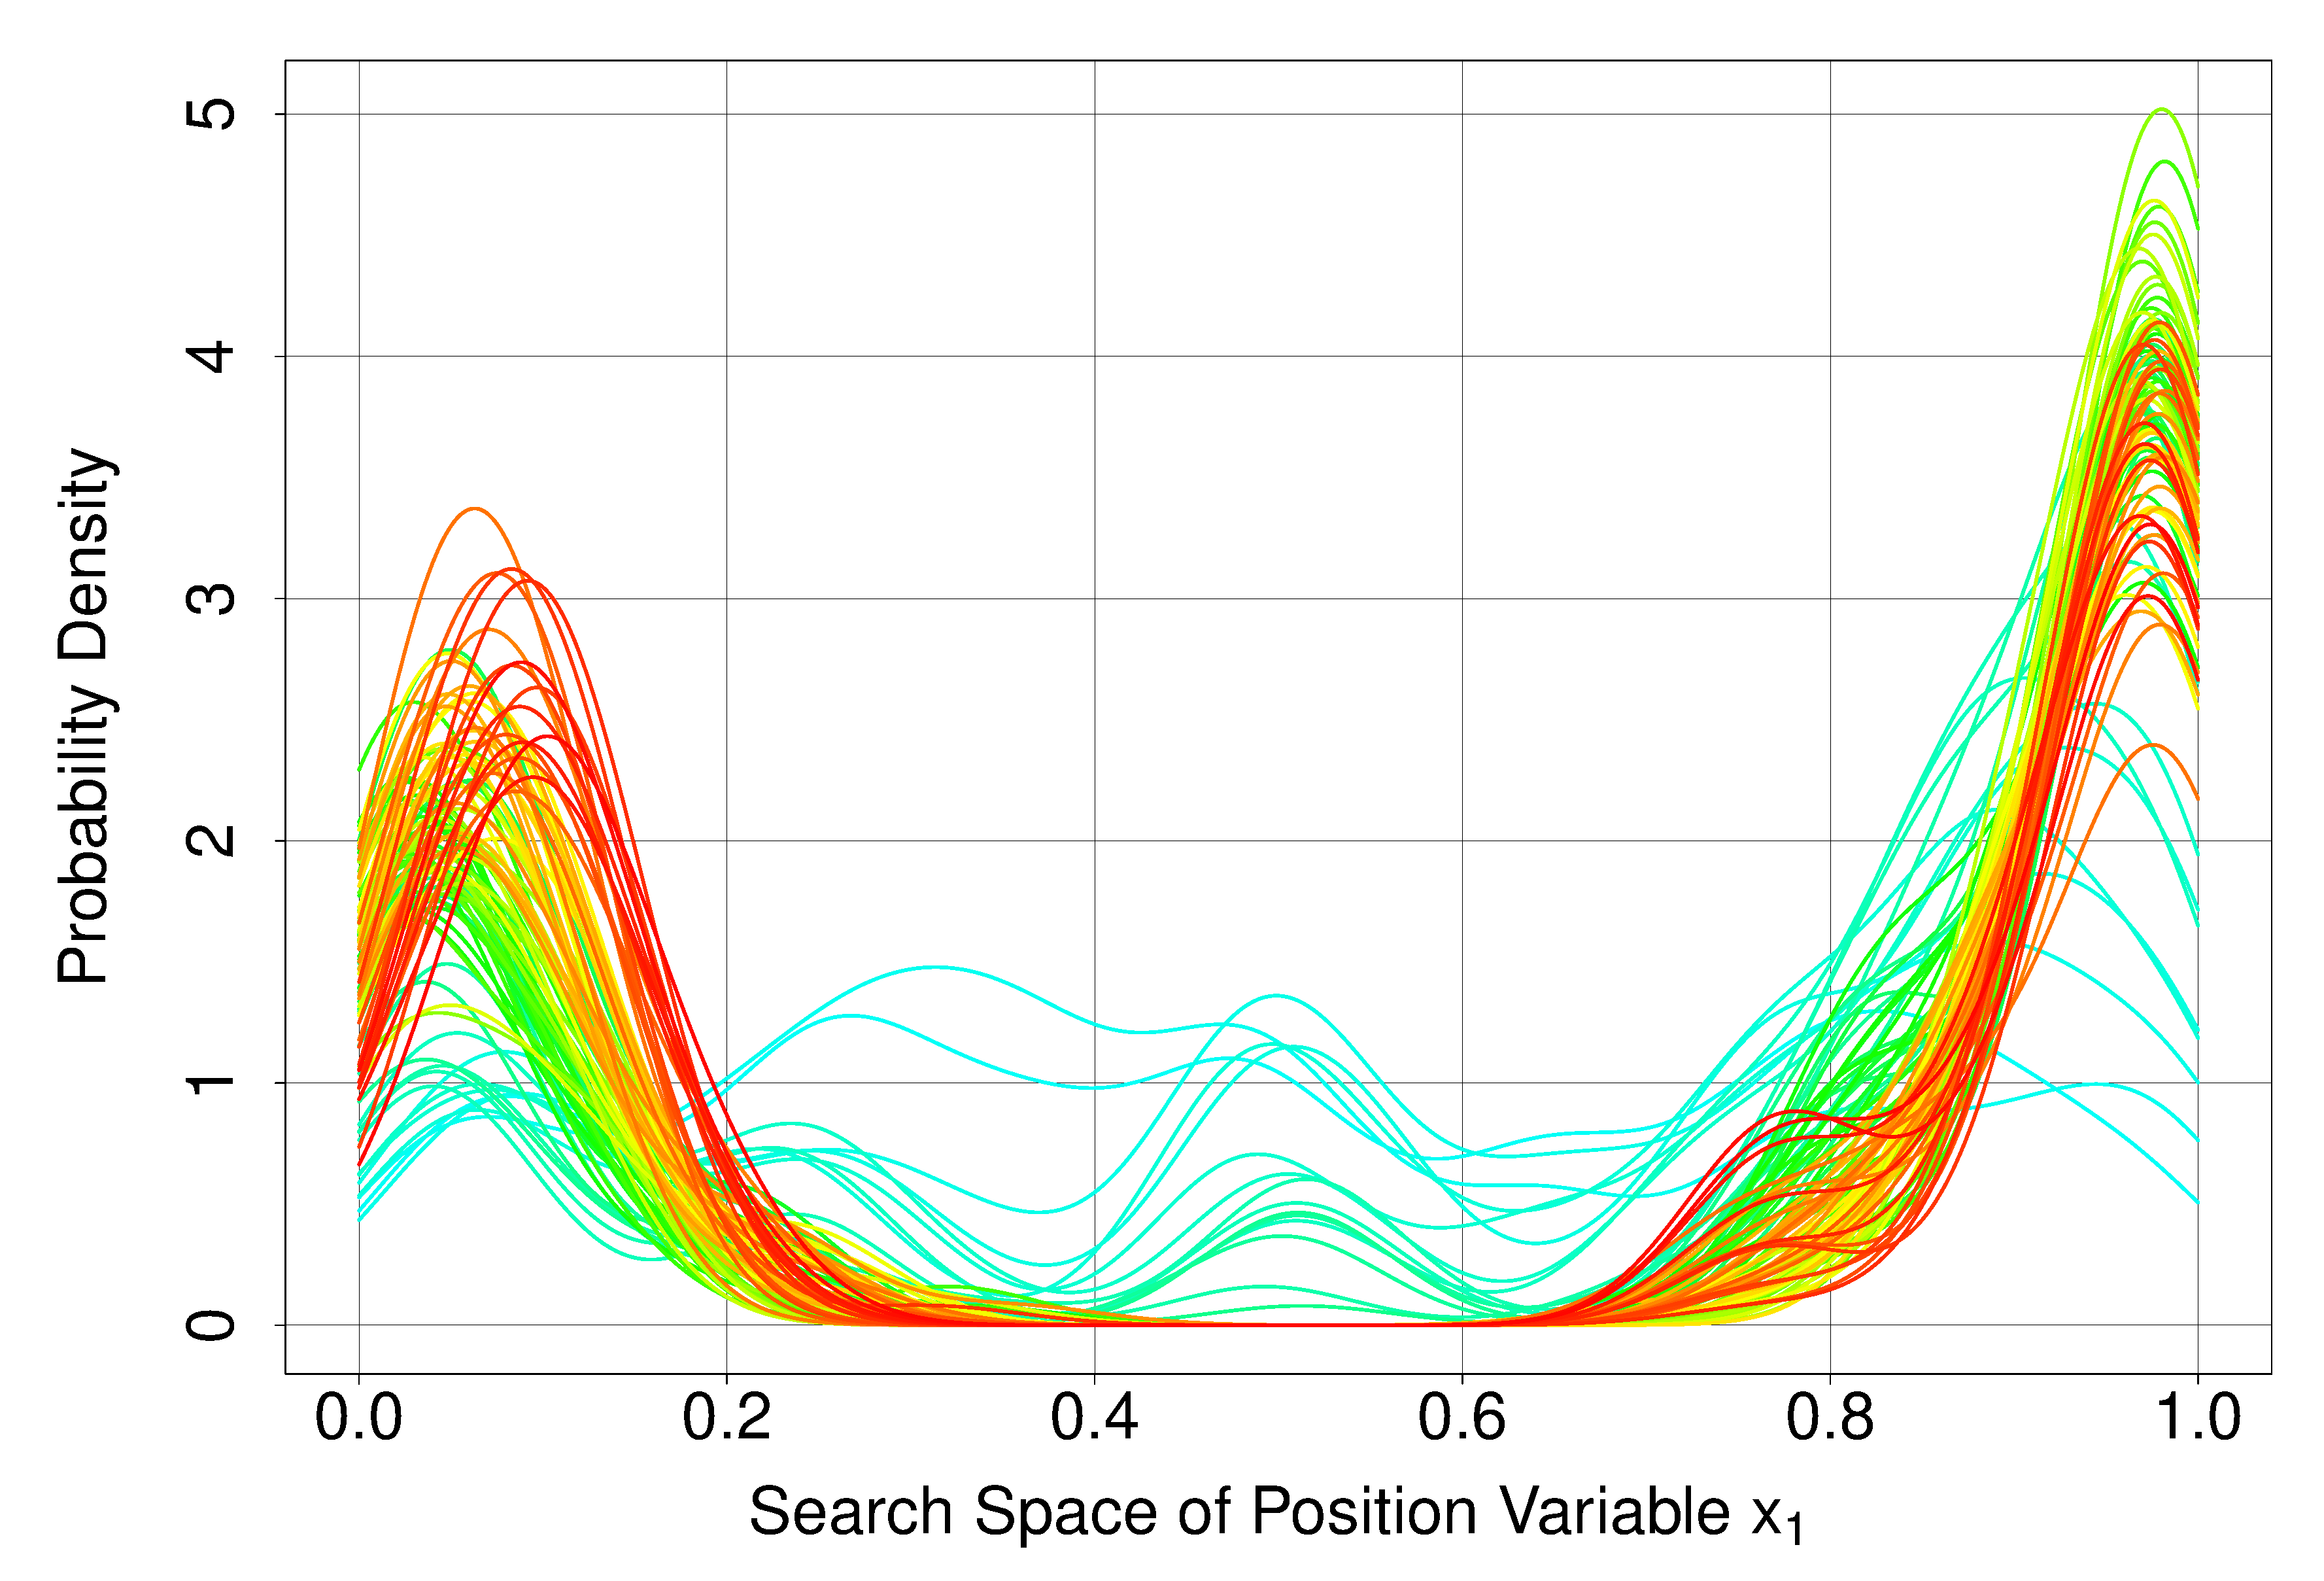
\includegraphics[width=1\linewidth]{../figures/WFG7_var1_pdf_trend.eps}\\
\centering
\hspace{0.2in} \includegraphics[width=0.8\linewidth]{../figures/color_bar_100ver.eps}
\begin{center}
{\footnotesize (a) 位置変数$x_1$における推定された確率密度関数の推移}
\end{center}
\end{minipage}
\begin{minipage}{0.49\hsize}
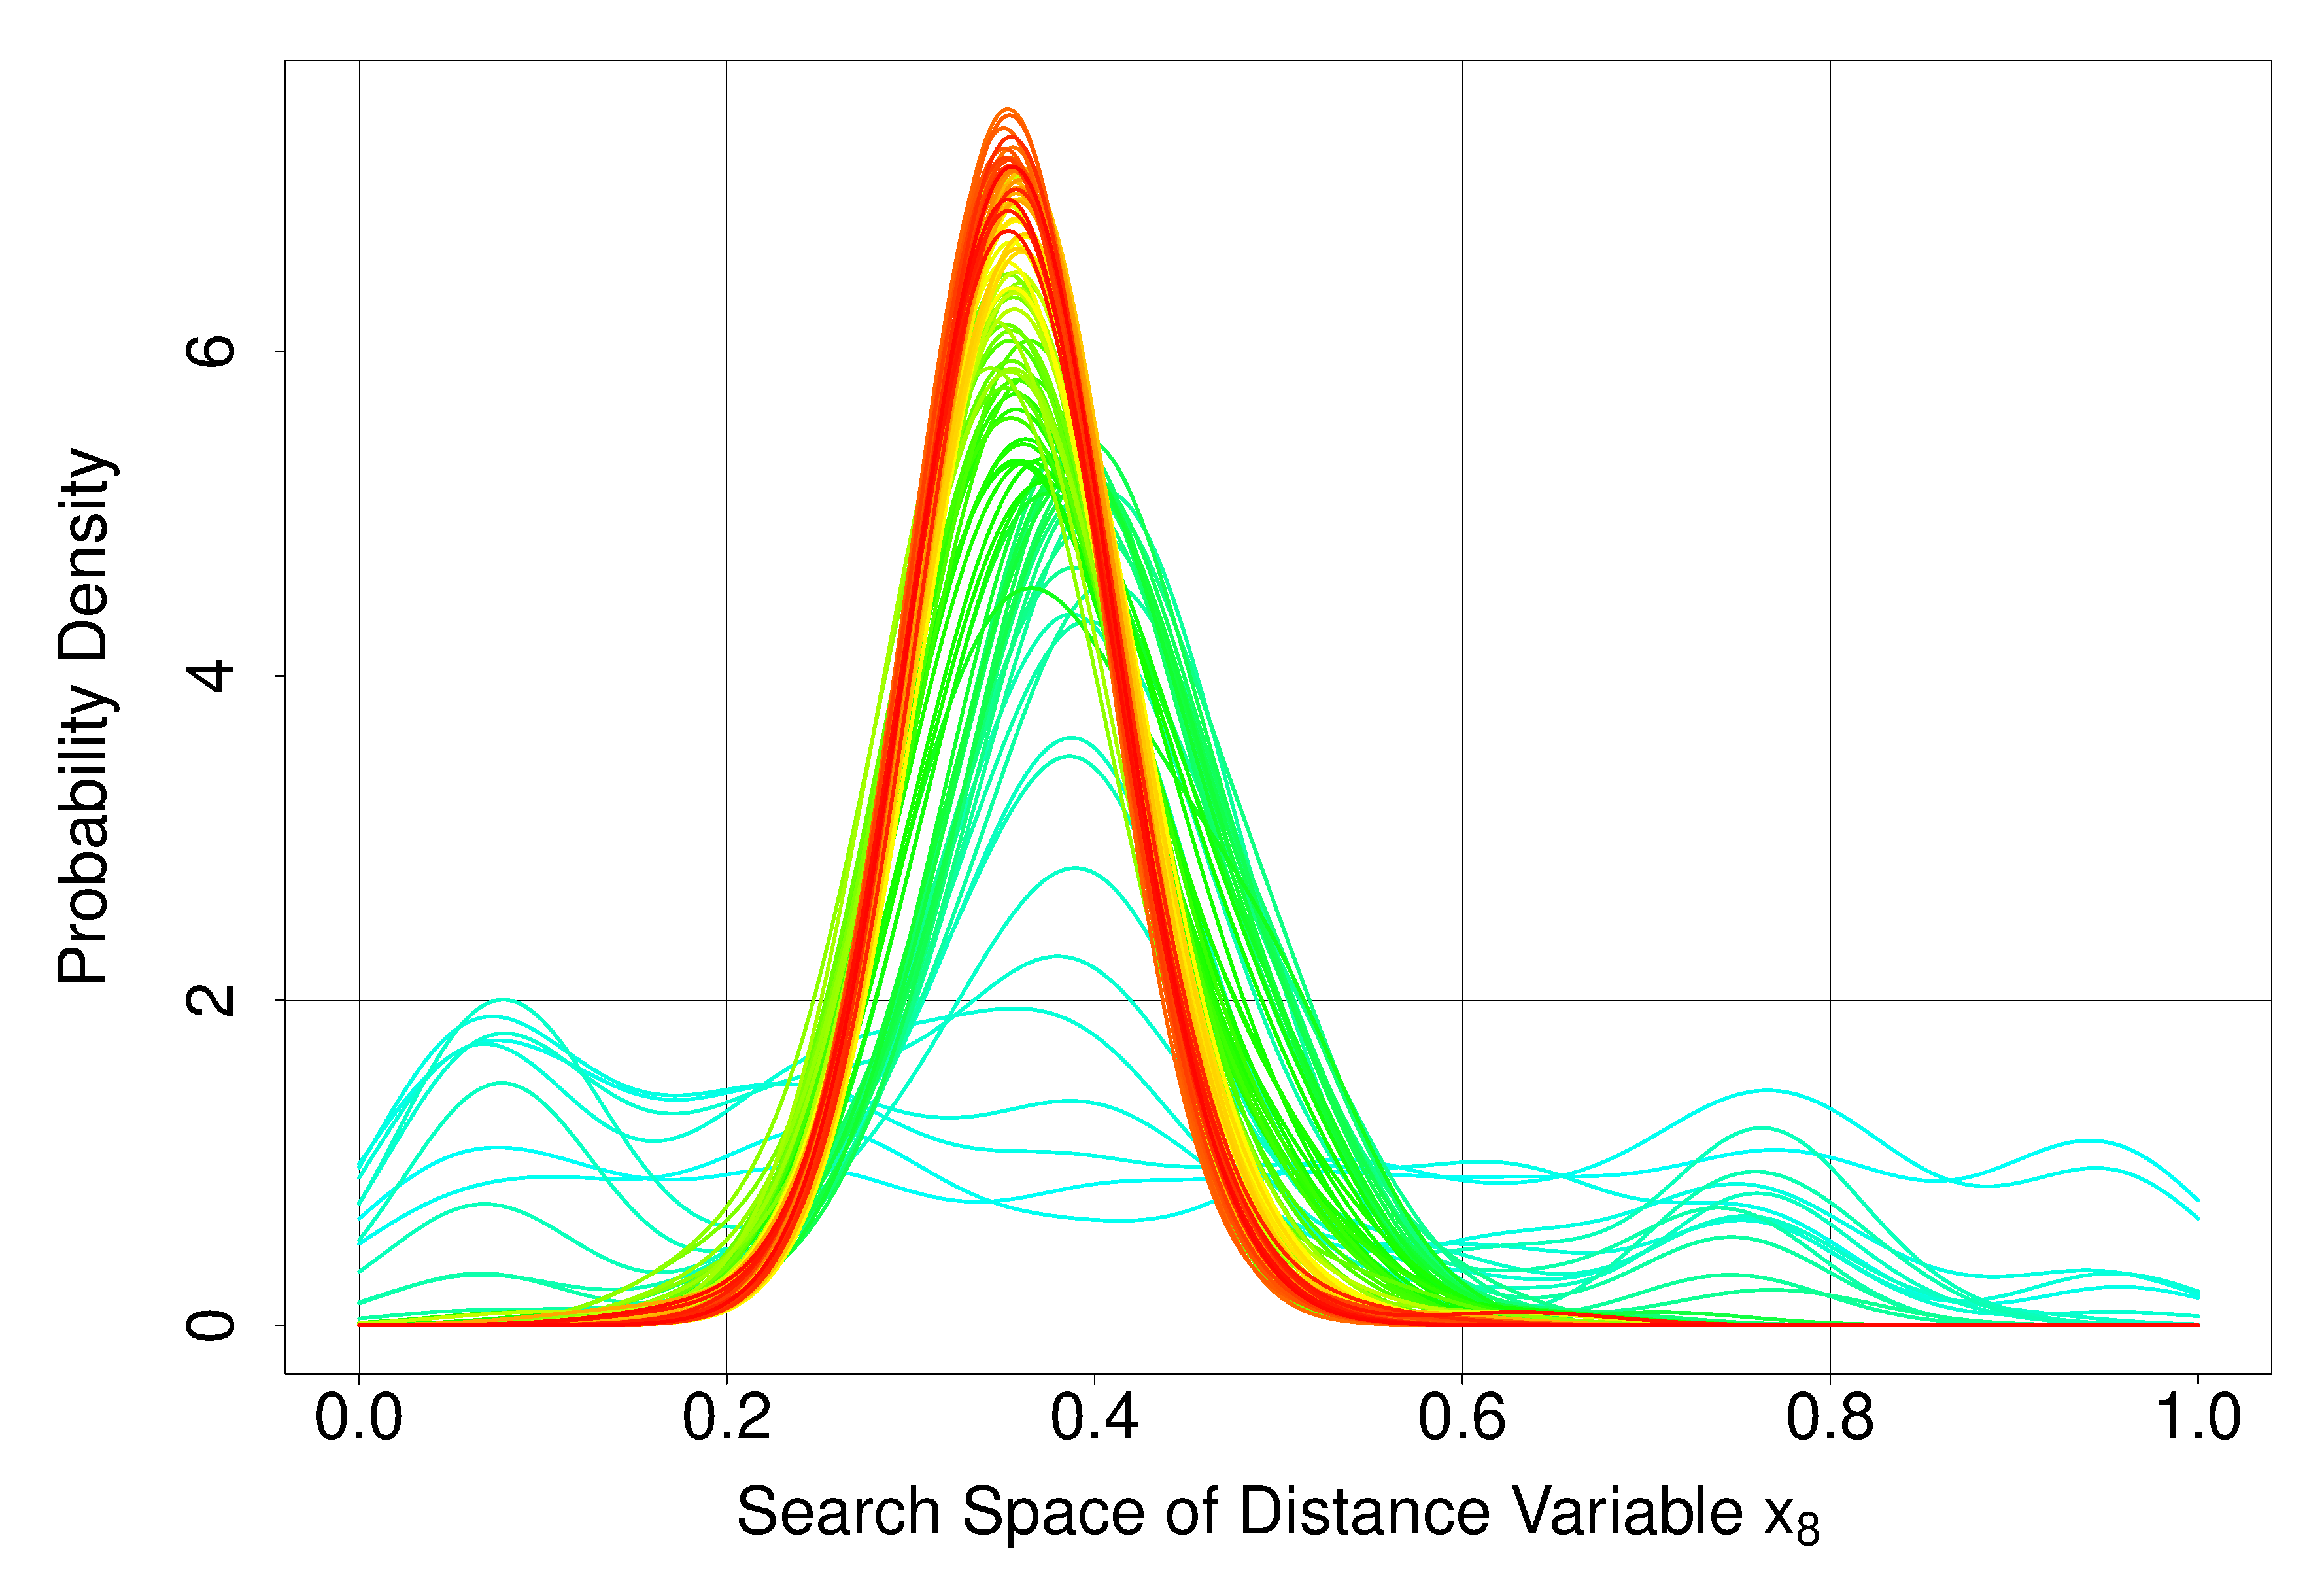
\includegraphics[width=1\linewidth]{../figures/WFG7_var8_pdf_trend.eps}\\
\centering
\hspace{0.2in} \includegraphics[width=0.8\linewidth]{../figures/color_bar_100ver.eps}
\begin{center}
{\footnotesize (b) 距離変数$x_{8}$における推定された確率密度関数の推移}
\end{center}
\end{minipage}
\caption{ePDFを用いた場合のWFG7における推定された確率密度関数の世代ごとの推移}
\label{pdf_trans_wfg7}
\end{minipage}
\label{fig:nondom_sol}
\end{figure*}

\afterpage{\clearpage}


\Figref{fig:nondoms_wfg7}はWFG7において,最終的に得られた非劣解集合を示している.
紫の線で示したものが真のパレートフロントの形状である.
どの場合においても,ある程度パレートフロントを覆うように非劣解が得られているものの,SDで得られた非劣解集合はややパレートフロントから離れた位置にも非劣解が存在することが分かる.
これらの解がGD悪化の原因であると考えられる.
また,GD,IGDは差が見られるものの実際に得られた非劣解集合には大きな違いは見られなかった.

\Figref{digi_trans_wfg7}は,SDにおける設計変数空間の分割数の世代ごとの推移を示している.
縦軸は設計変数の分割数を示しており,大きな値ほど細かく離散化されていることを表す.
また,赤線で示した推移はWFG7において,目的関数空間での位置を司る変数(位置変数)である$x_1$-$x_6$の推移を示しており,青線で示した推移は目的関数空間での距離を司る変数(距離変数)である$x_7$-$x_{10}$を示している.
\Figref{digi_trans_wfg7}より,赤で示した位置変数$x_1$-$x_6$は1つを除いて常に粗く離散化されている一方で,青で示した距離変数$x_7$-$x_{10}$は世代を経るごとに細かい離散化に推移していることが分かる.
\Figref{fig:nondoms_wfg7}の非劣解集合の分布より,位置変数は粗く離散化されても多様性が著しく減少することはないことが分かる.
このことから,DTLZ3と同様に,細かい離散化が必要である設計変数とそうでない設計変数を識別することができていると考えられる.

\Figref{pdf_trans_wfg7}は,ePDFを用いた場合に各世代におけるある設計変数空間の分布について推定された確率密度関数を示しており,(a)は位置変数である$x_1$,(b)は距離変数である$x_{8}$について得られた確率密度関数を示している.
縦軸は確率密度,横軸は設計変数空間を正規化空間に射影した際の探索空間を示しており[0,1]の範囲であり,確率密度関数の色は推定された世代を示している.
ePDFを用いた適応的離散化では,確率密度が高いほど細かく離散化が行われる.
\Figref{pdf_trans}(a)より,位置変数$x_1$では世代を経るごとに0.1,1付近の確率密度が高い値となっていることから,0.1,1付近の解は細かく離散化されていることが分かる.
また,密な分布が2つ検出することができている.
SDではこのように密な分布が複数存在する場合,特徴をうまく捉えることができないため,SDよりもGD,IGDが優れた結果となったことが考えられる.
\Figref{pdf_trans}(b)より,距離変数$x_8$では世代を経るごとに0.35付近の確率密度が高い値となっていることから,0.35付近の解は細かく離散化されていることが分かる.
この結果から,WFG7においてもePDFは期待したメカニズムが有効に機能しており,離散化することでGD・IGDが悪くなってしまうような問題に対しても,大きく探索性能を損なわなかったことが確認できた.


\clearpage

\subsubsection{Multi DTLZ4}

\Figref{multidtlz4_gd_transition},\ref{multidtlz4_igd_transition}はそれぞれMulti DTLZ4においてSD,ePDFを用いた適応的離散化手法と離散化制御を用いなかった場合に得られたGD,IGDの平均値の推移を示している.
\Figref{multidtlz4_gd_transition},\ref{multidtlz4_igd_transition}を見ると,GDではSDが優れた結果となっており,IGDではePDFが優れた結果となっていることが分かる.
この結果から,離散化の仕方の違いにより,収束性が向上する場合と多様性が向上する場合があることが分かった.

\Figref{fig:nondoms_multidtlz4}はMulti DTLZ4において,最終的に得られた非劣解集合を示している.
紫の線で示したものが真のパレートフロントの形状である.
どの場合においても,真のパレートフロントを覆うように非劣解が分布しており,IGDに差はあるものの多様性に大きな差はないことが分かる.
また,制御なしの非劣解集合では,ややパレートフロントから離れた位置にも非劣解が分布しており,GD悪化の一因であると考えられる.

\Figref{digi_trans_multidtlz4}は,SDにおける設計変数空間の分割数の世代ごとの推移を示している.
縦軸は設計変数の分割数を示しており,大きな値ほど細かく離散化されていることを表す.
また,赤線で示した推移はWFG7において,目的関数空間での位置を司る変数(位置変数)である$x_1$,$x_2$の推移を示しており,青線で示した推移は目的関数空間での距離を司る変数(距離変数)である$x_3$-$x_{38}$を示している.
\Figref{digi_trans_multidtlz4}より,赤で示した位置変数$x_1$,$x_2$は世代を経るごとに細かい離散化に推移していることが分かる.
Multi DTLZ4は式の構造上,解の多様性を向上させるためには位置変数に細かい粒度が必要とされる.
したがって,SDを用いた適応的離散化では 必要な分割数に適応的に変化することで効率良い探索が行えており,期待したメカニズムが有効に機能していることが分かる.
一方で,距離変数$x_3$-$x_{38}$は,粗い離散化がされているものと細かい離散化がされているもので非常に大きくばらついていることが分かる.
Multi DTLZ4は距離変数の最適値が二つ存在する問題である.
そのため,設計変数空間に密な分布が二つ存在することがあり,その場合,設計変数空間の解の分散が大きくなってしまうためSDも大きくなり,粗く離散化されてしまう.
真の最適値に到達するためには非常に細かい粒度が必要とされるが,このようにうまく分布の特徴を捉える事ができていないために,粗い離散化を行ってしまっていることが分かる.
この結果から,設計変数空間に密な分布が複数存在するような問題の場合,SDはうまく機能しない可能性があることが分かった.

\begin{figure*}[!ht]
\begin{tabular}{cc}
\begin{minipage}{0.49\hsize}
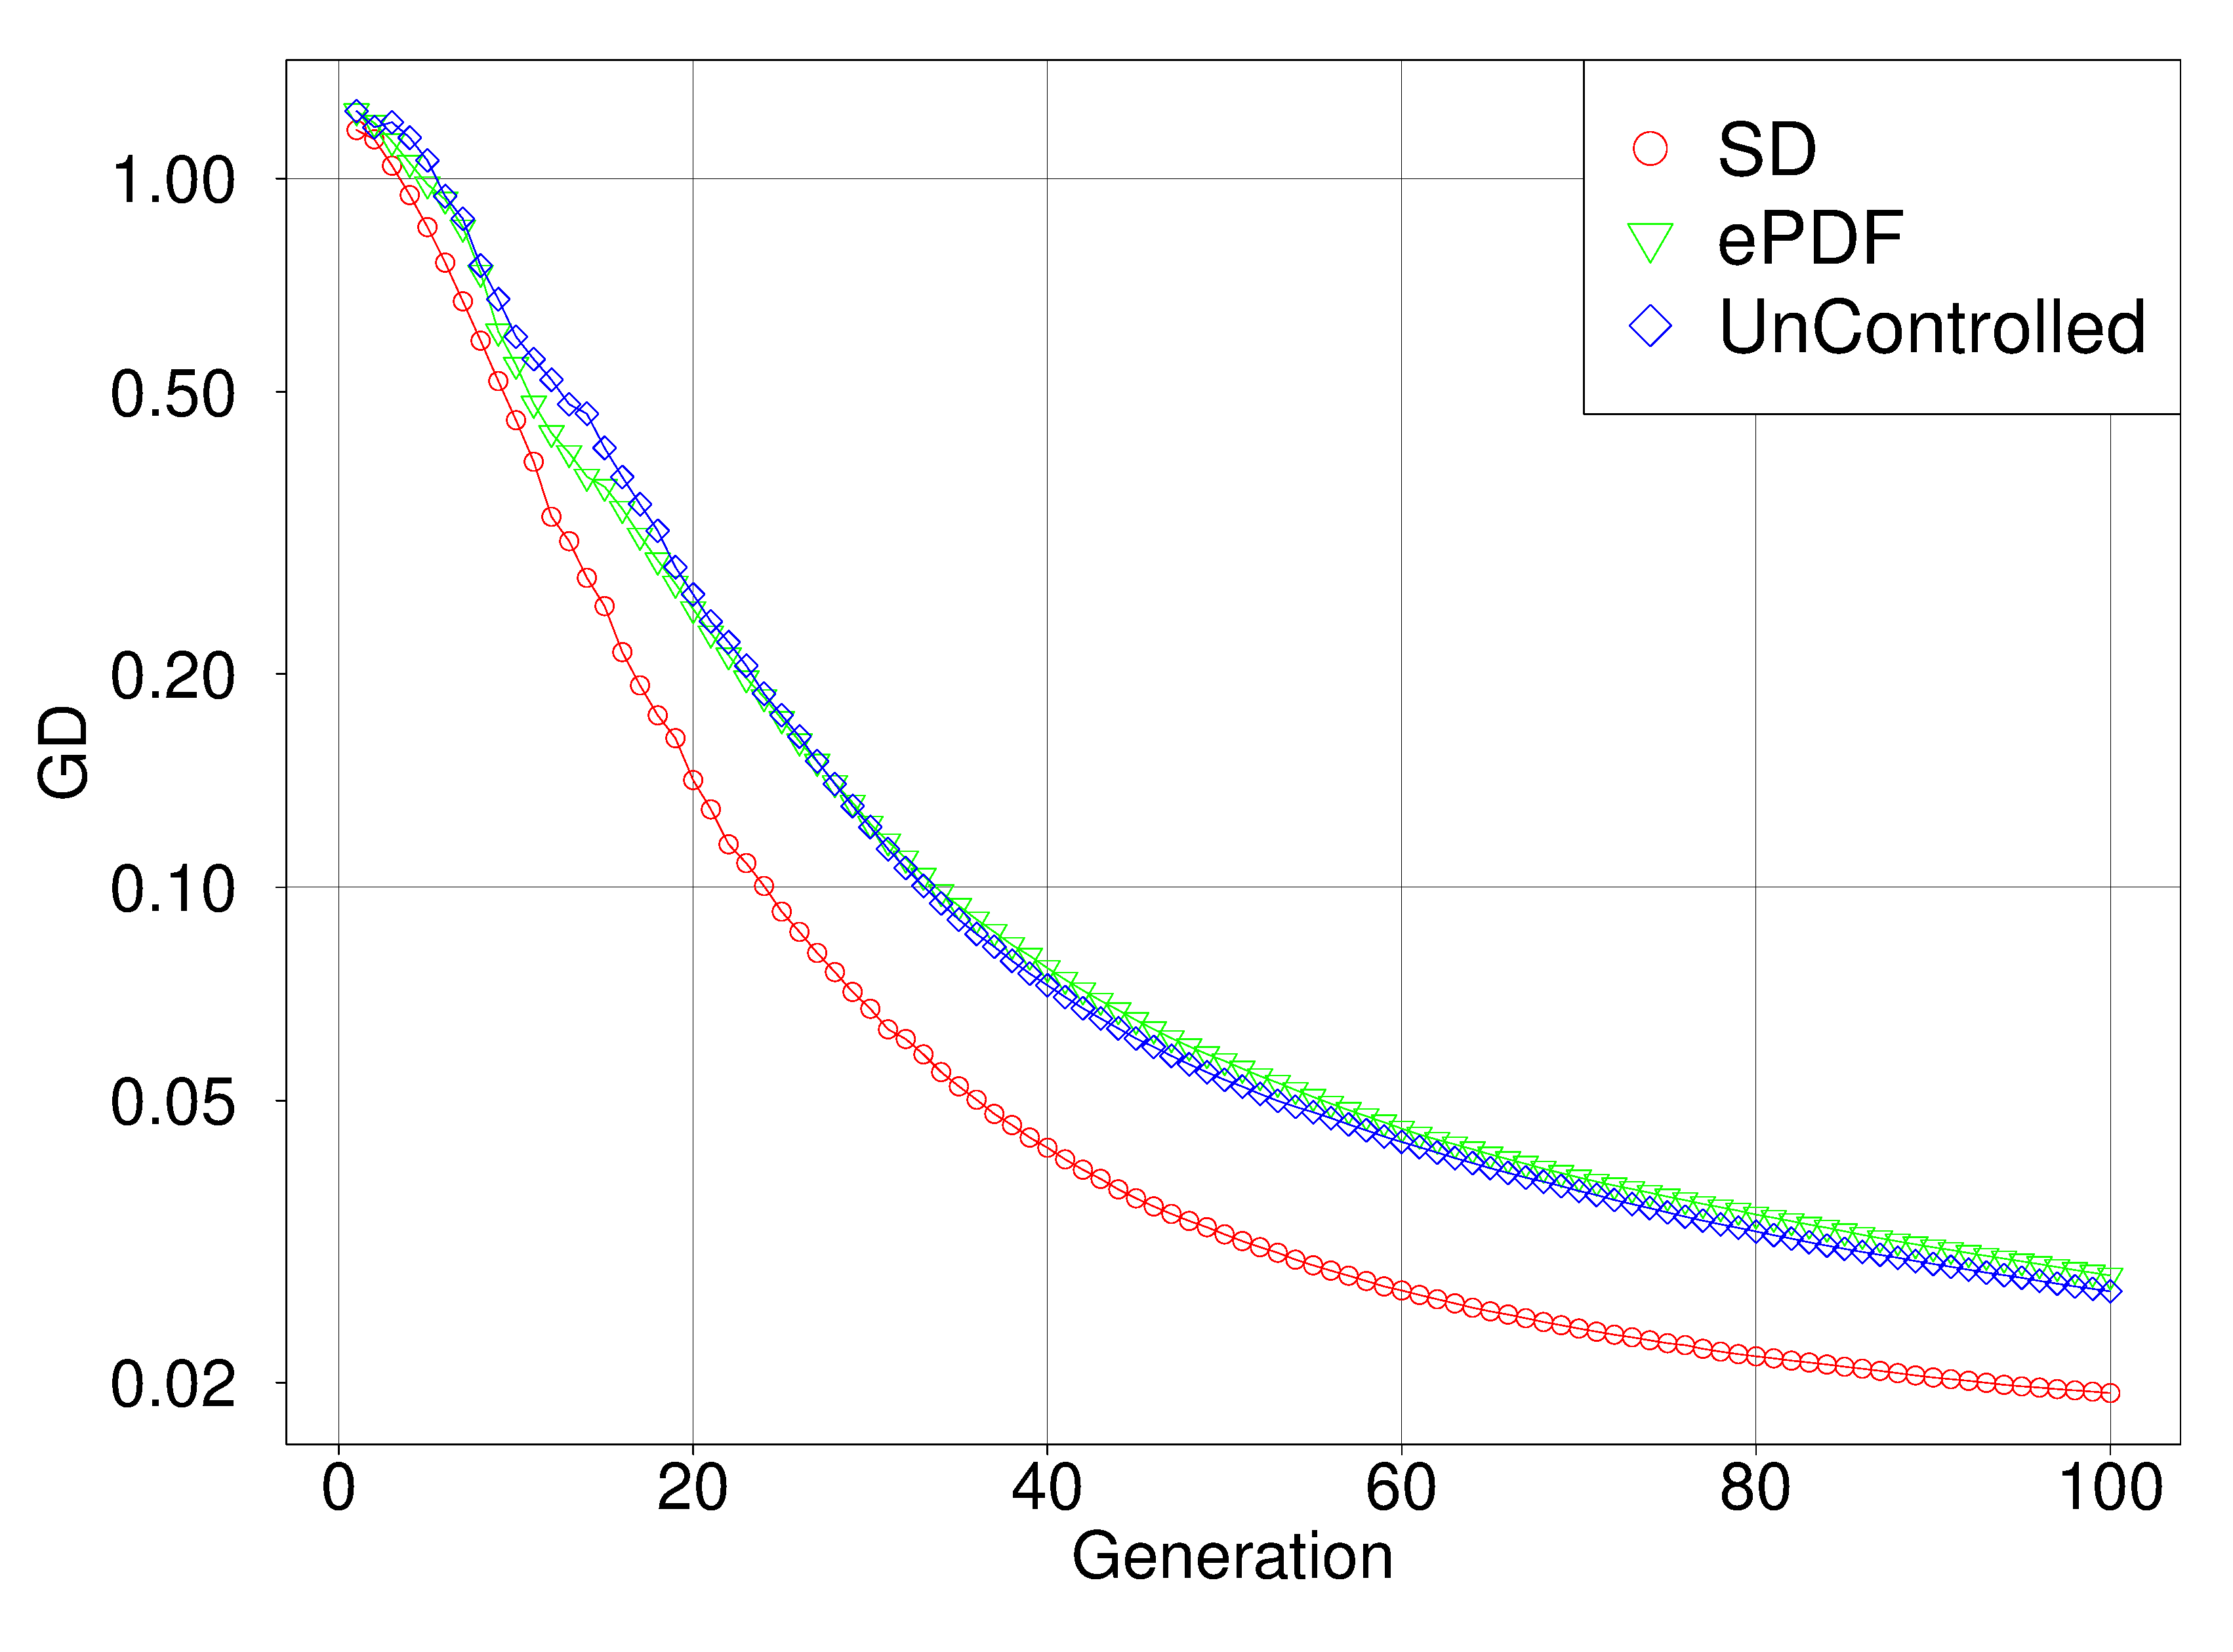
\includegraphics[width=1\linewidth]{../figures/multi_DTLZ4_GD.eps}
\caption{適応的離散化手法を用いた場合と用いない場合のMulti DTLZ4におけるGDの推移}
\label{multidtlz4_gd_transition}
\end{minipage}
\begin{minipage}{0.49\hsize}
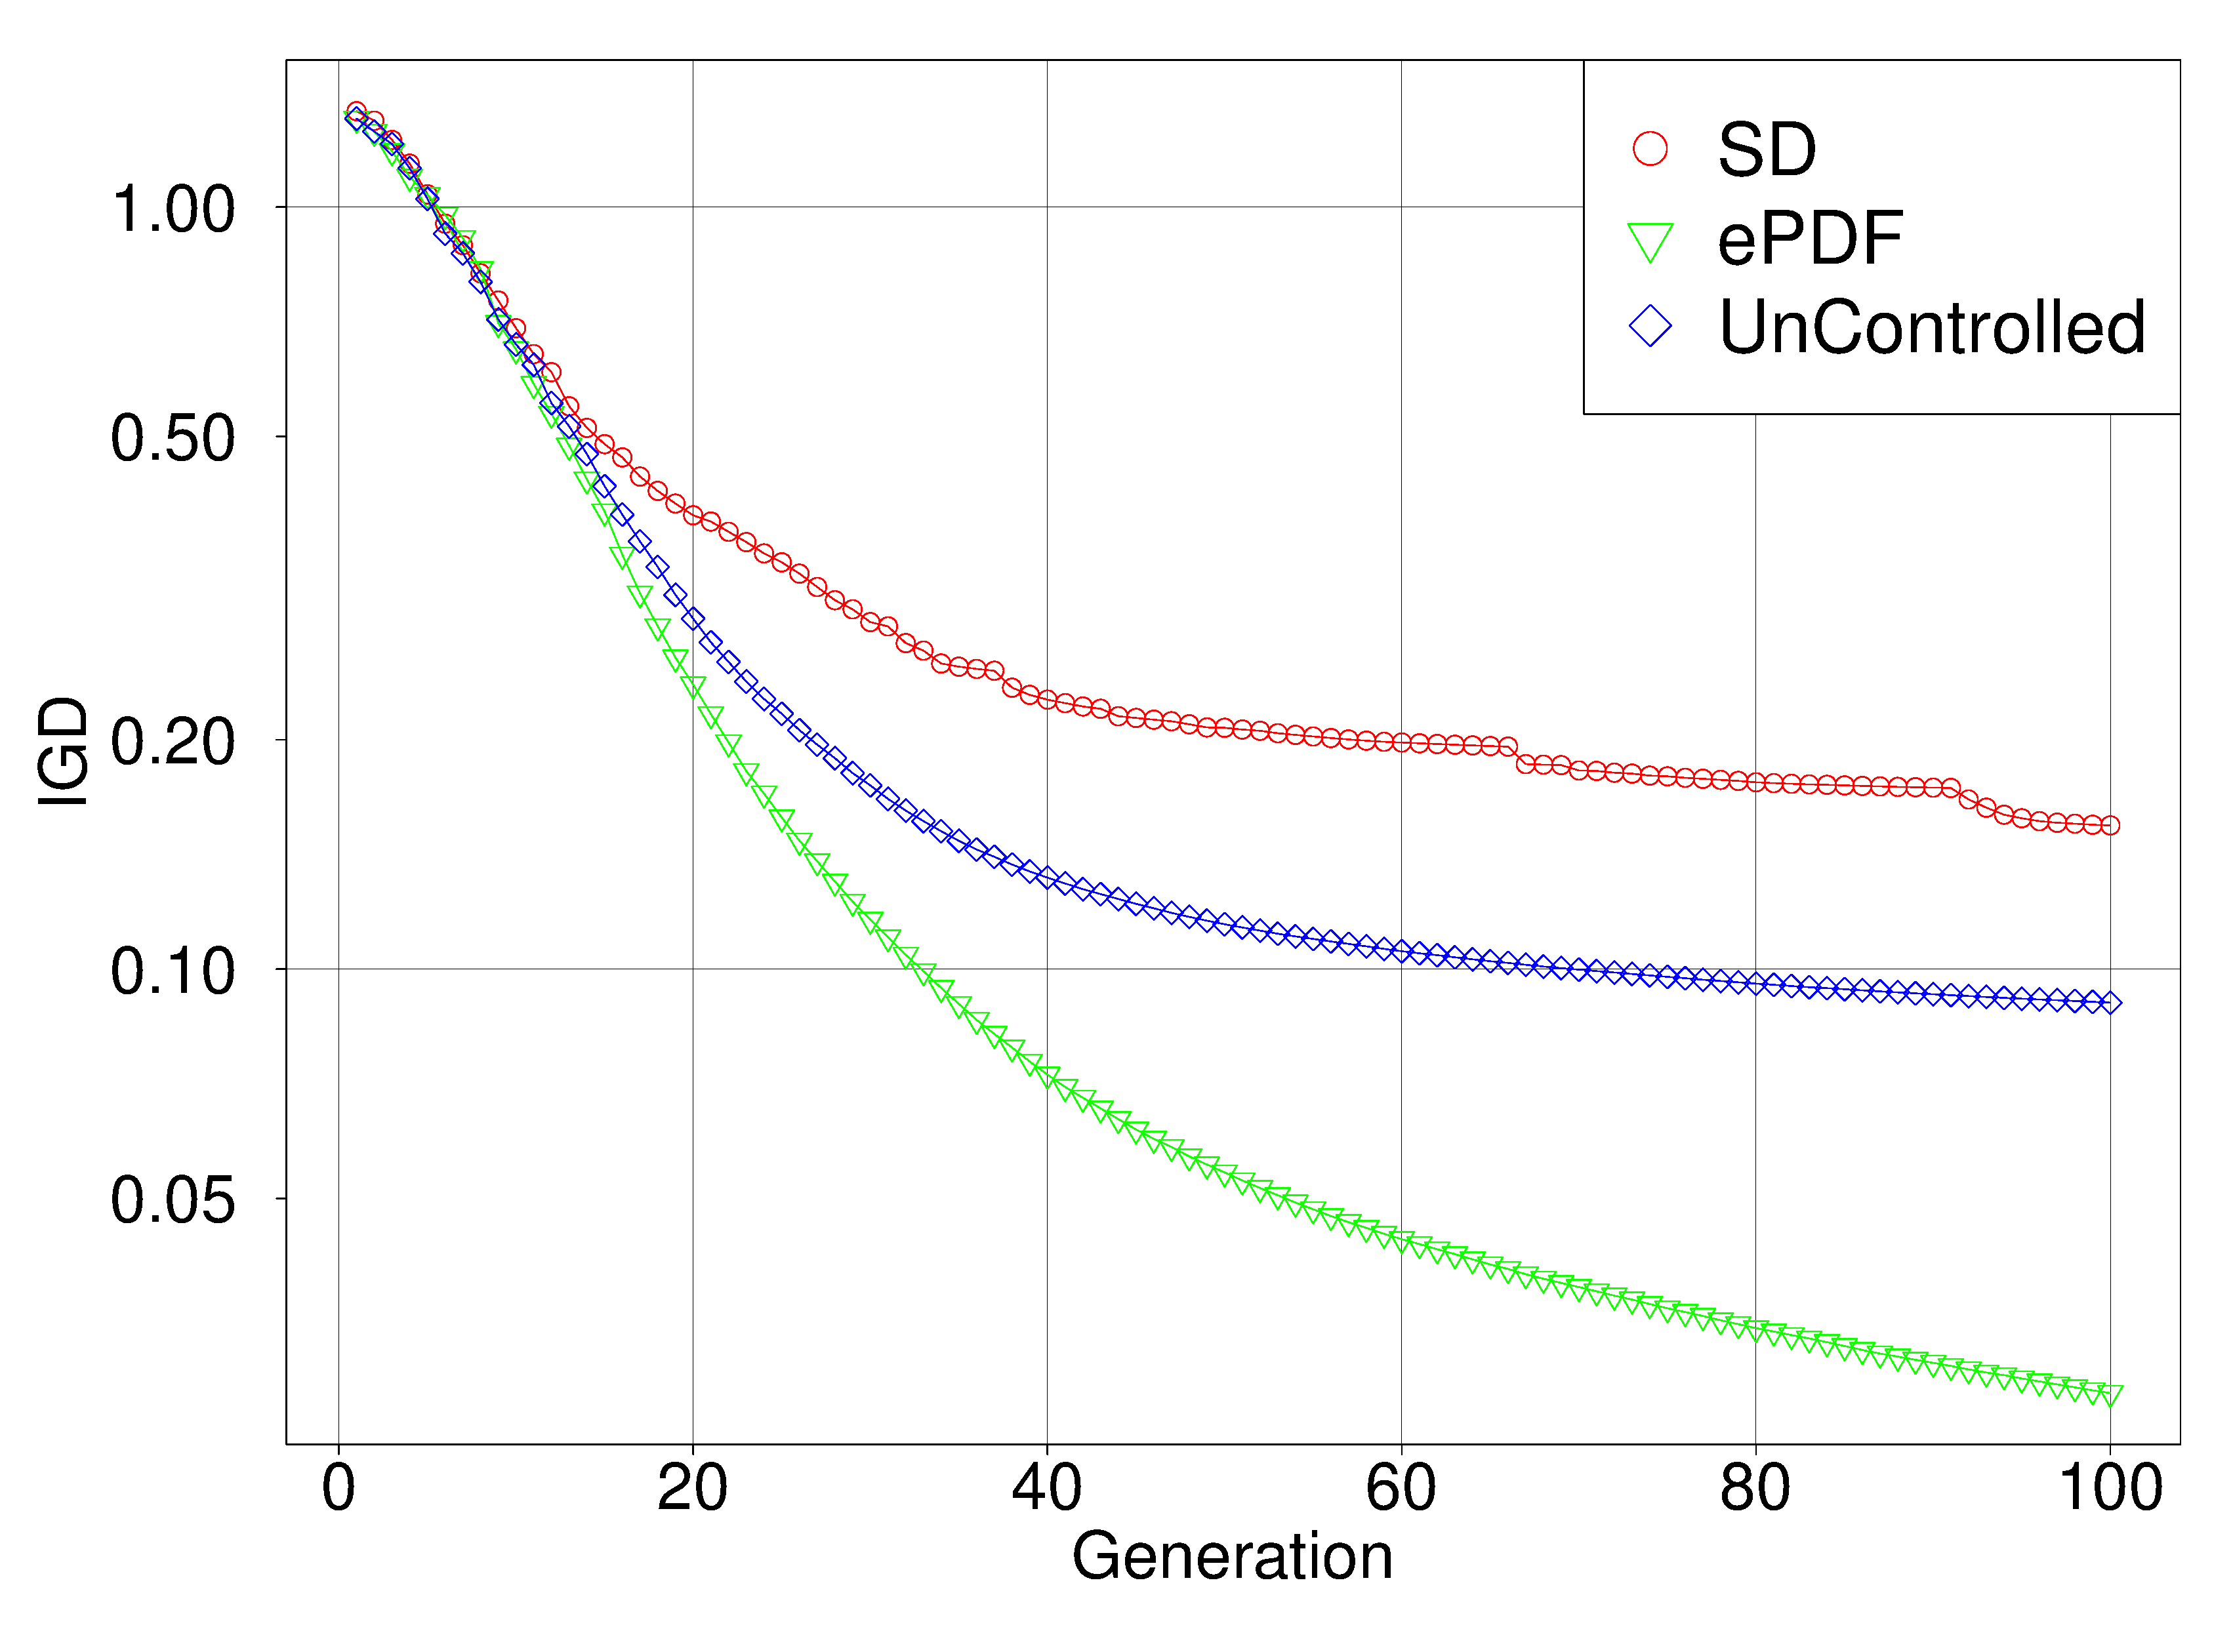
\includegraphics[width=1\linewidth]{../figures/multi_DTLZ4_IGD.eps}
\caption{適応的離散化手法を用いた場合と用いない場合のModified DTLZ4におけるIGDの推移}
\label{multidtlz4_igd_transition}
\end{minipage}
\end{tabular}
\end{figure*}

\begin{figure*}[htbp]
\begin{tabular}{cc}
\begin{minipage}{0.33\hsize}
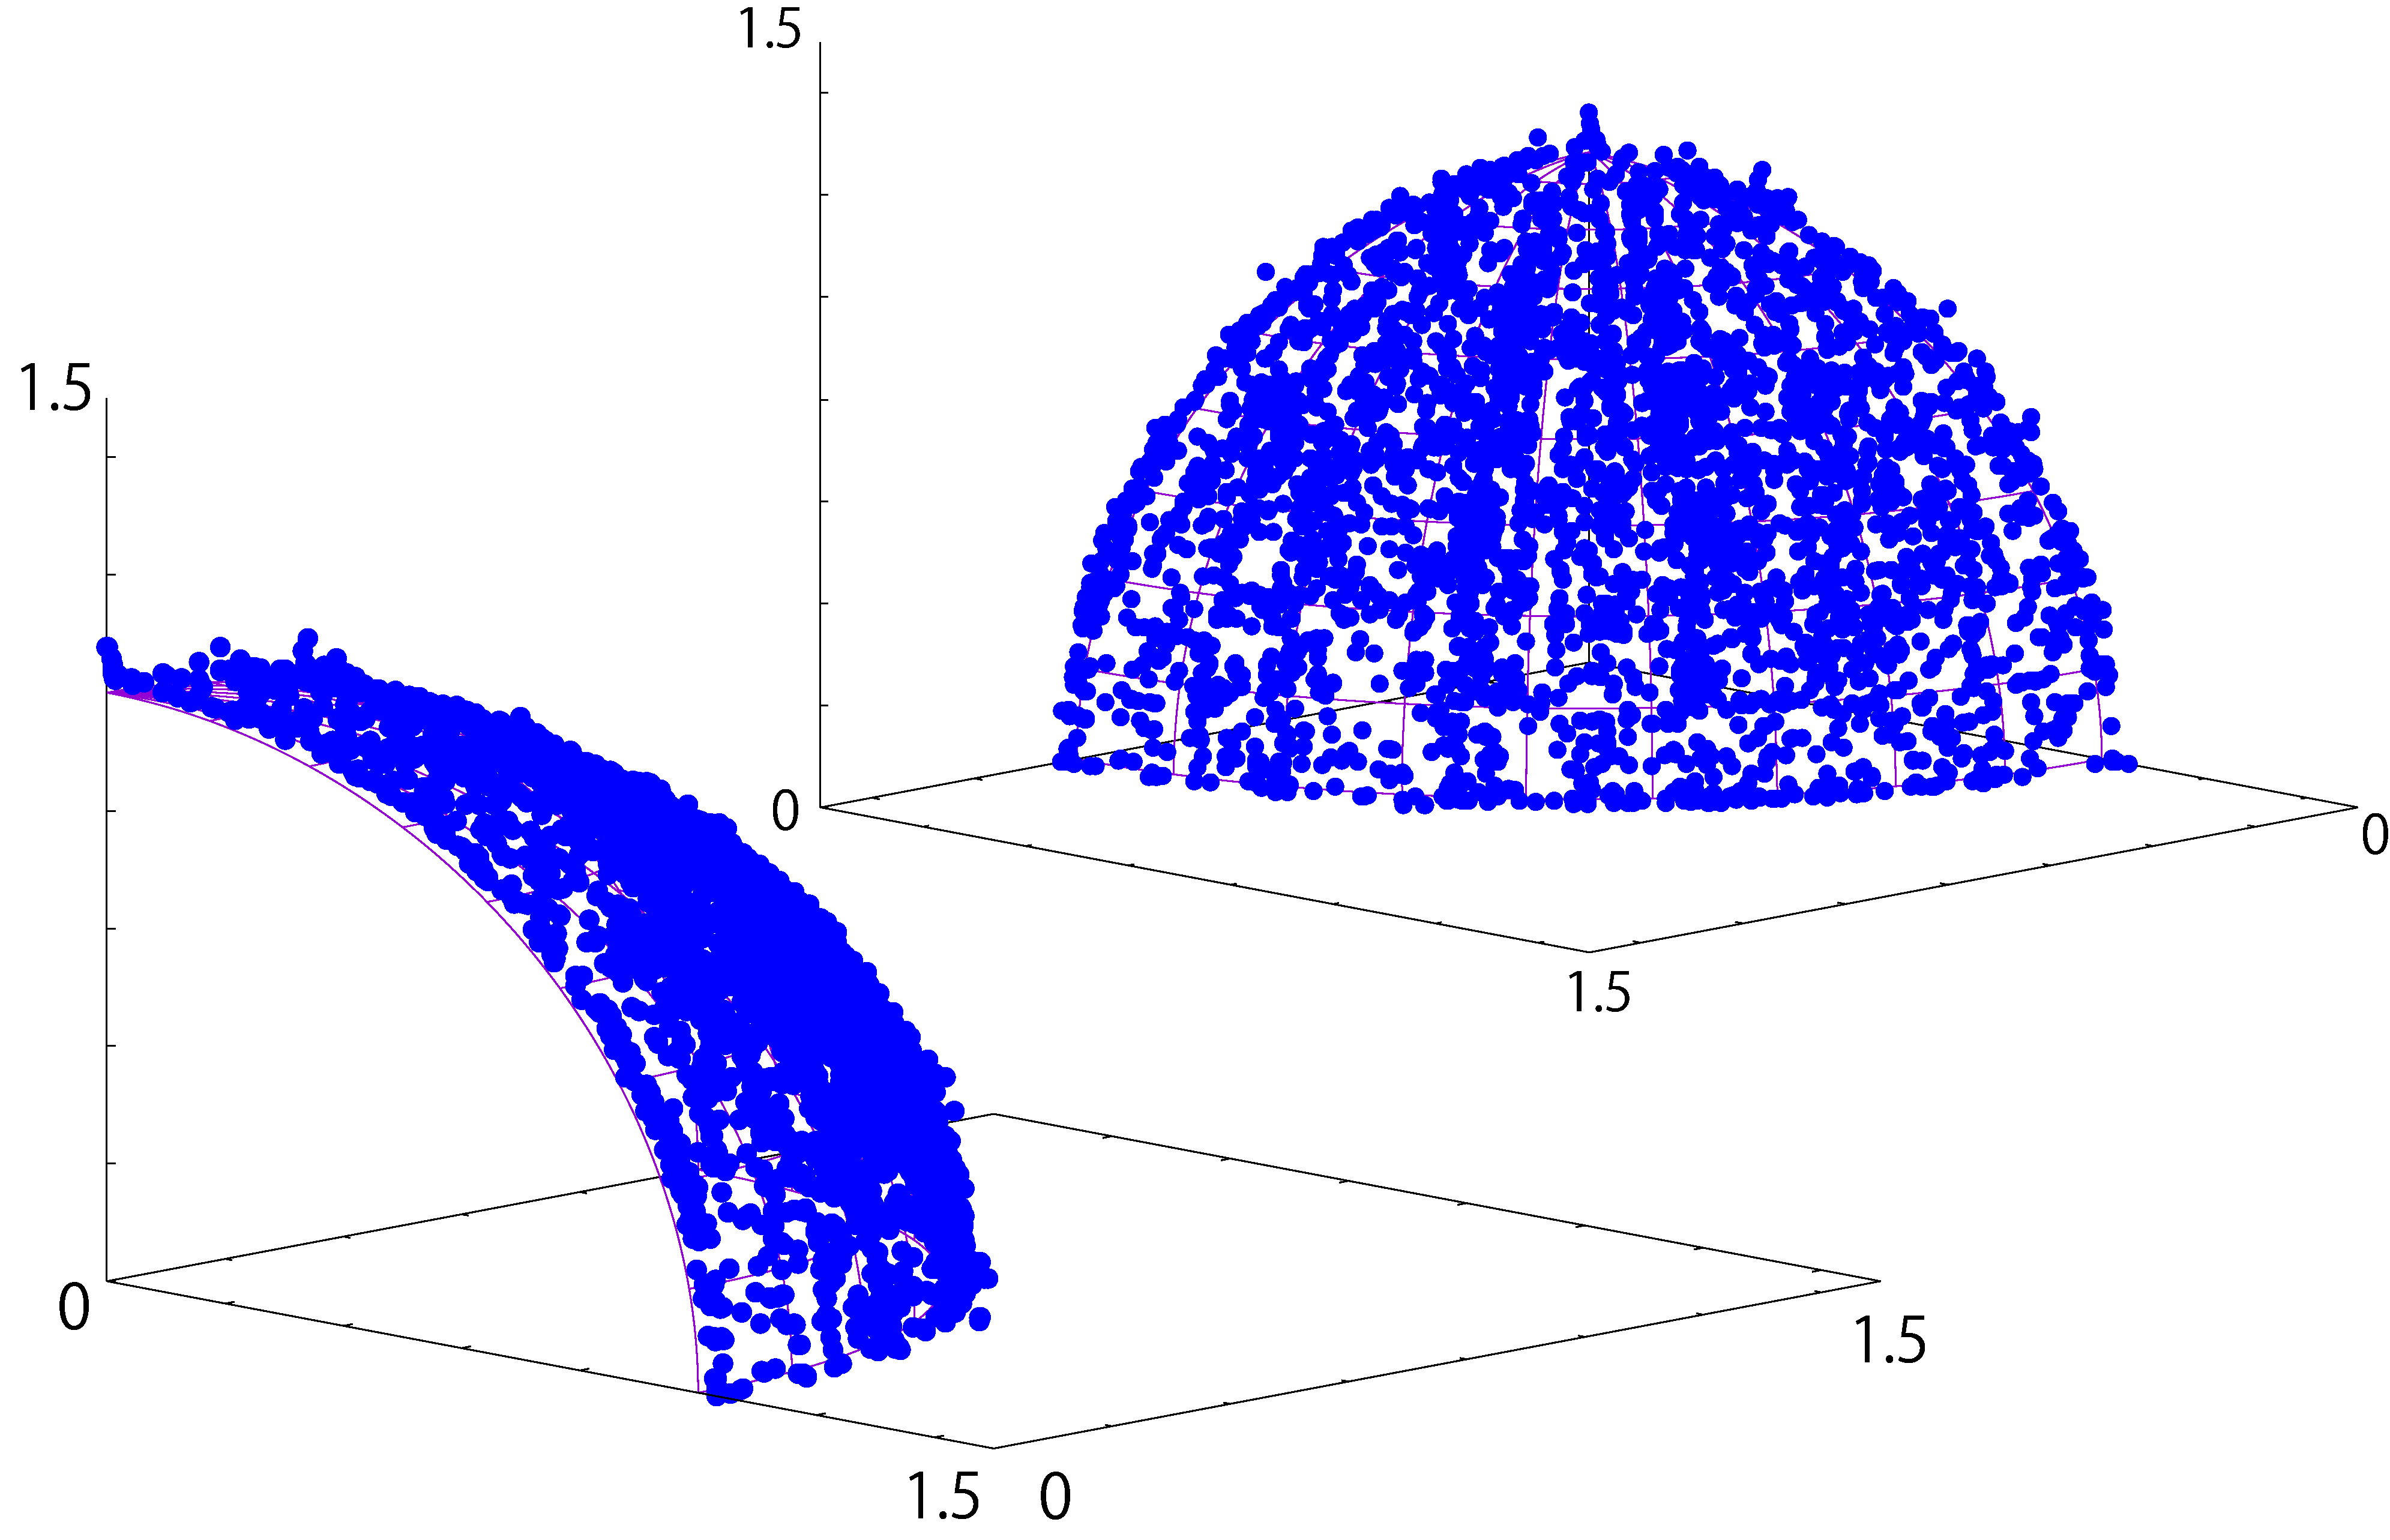
\includegraphics[width=1\linewidth]{../figures/multidtlz4_sd_double.pdf}
\begin{center}
{\footnotesize (a) SD}
\end{center}
\end{minipage}
\begin{minipage}{0.33\hsize}
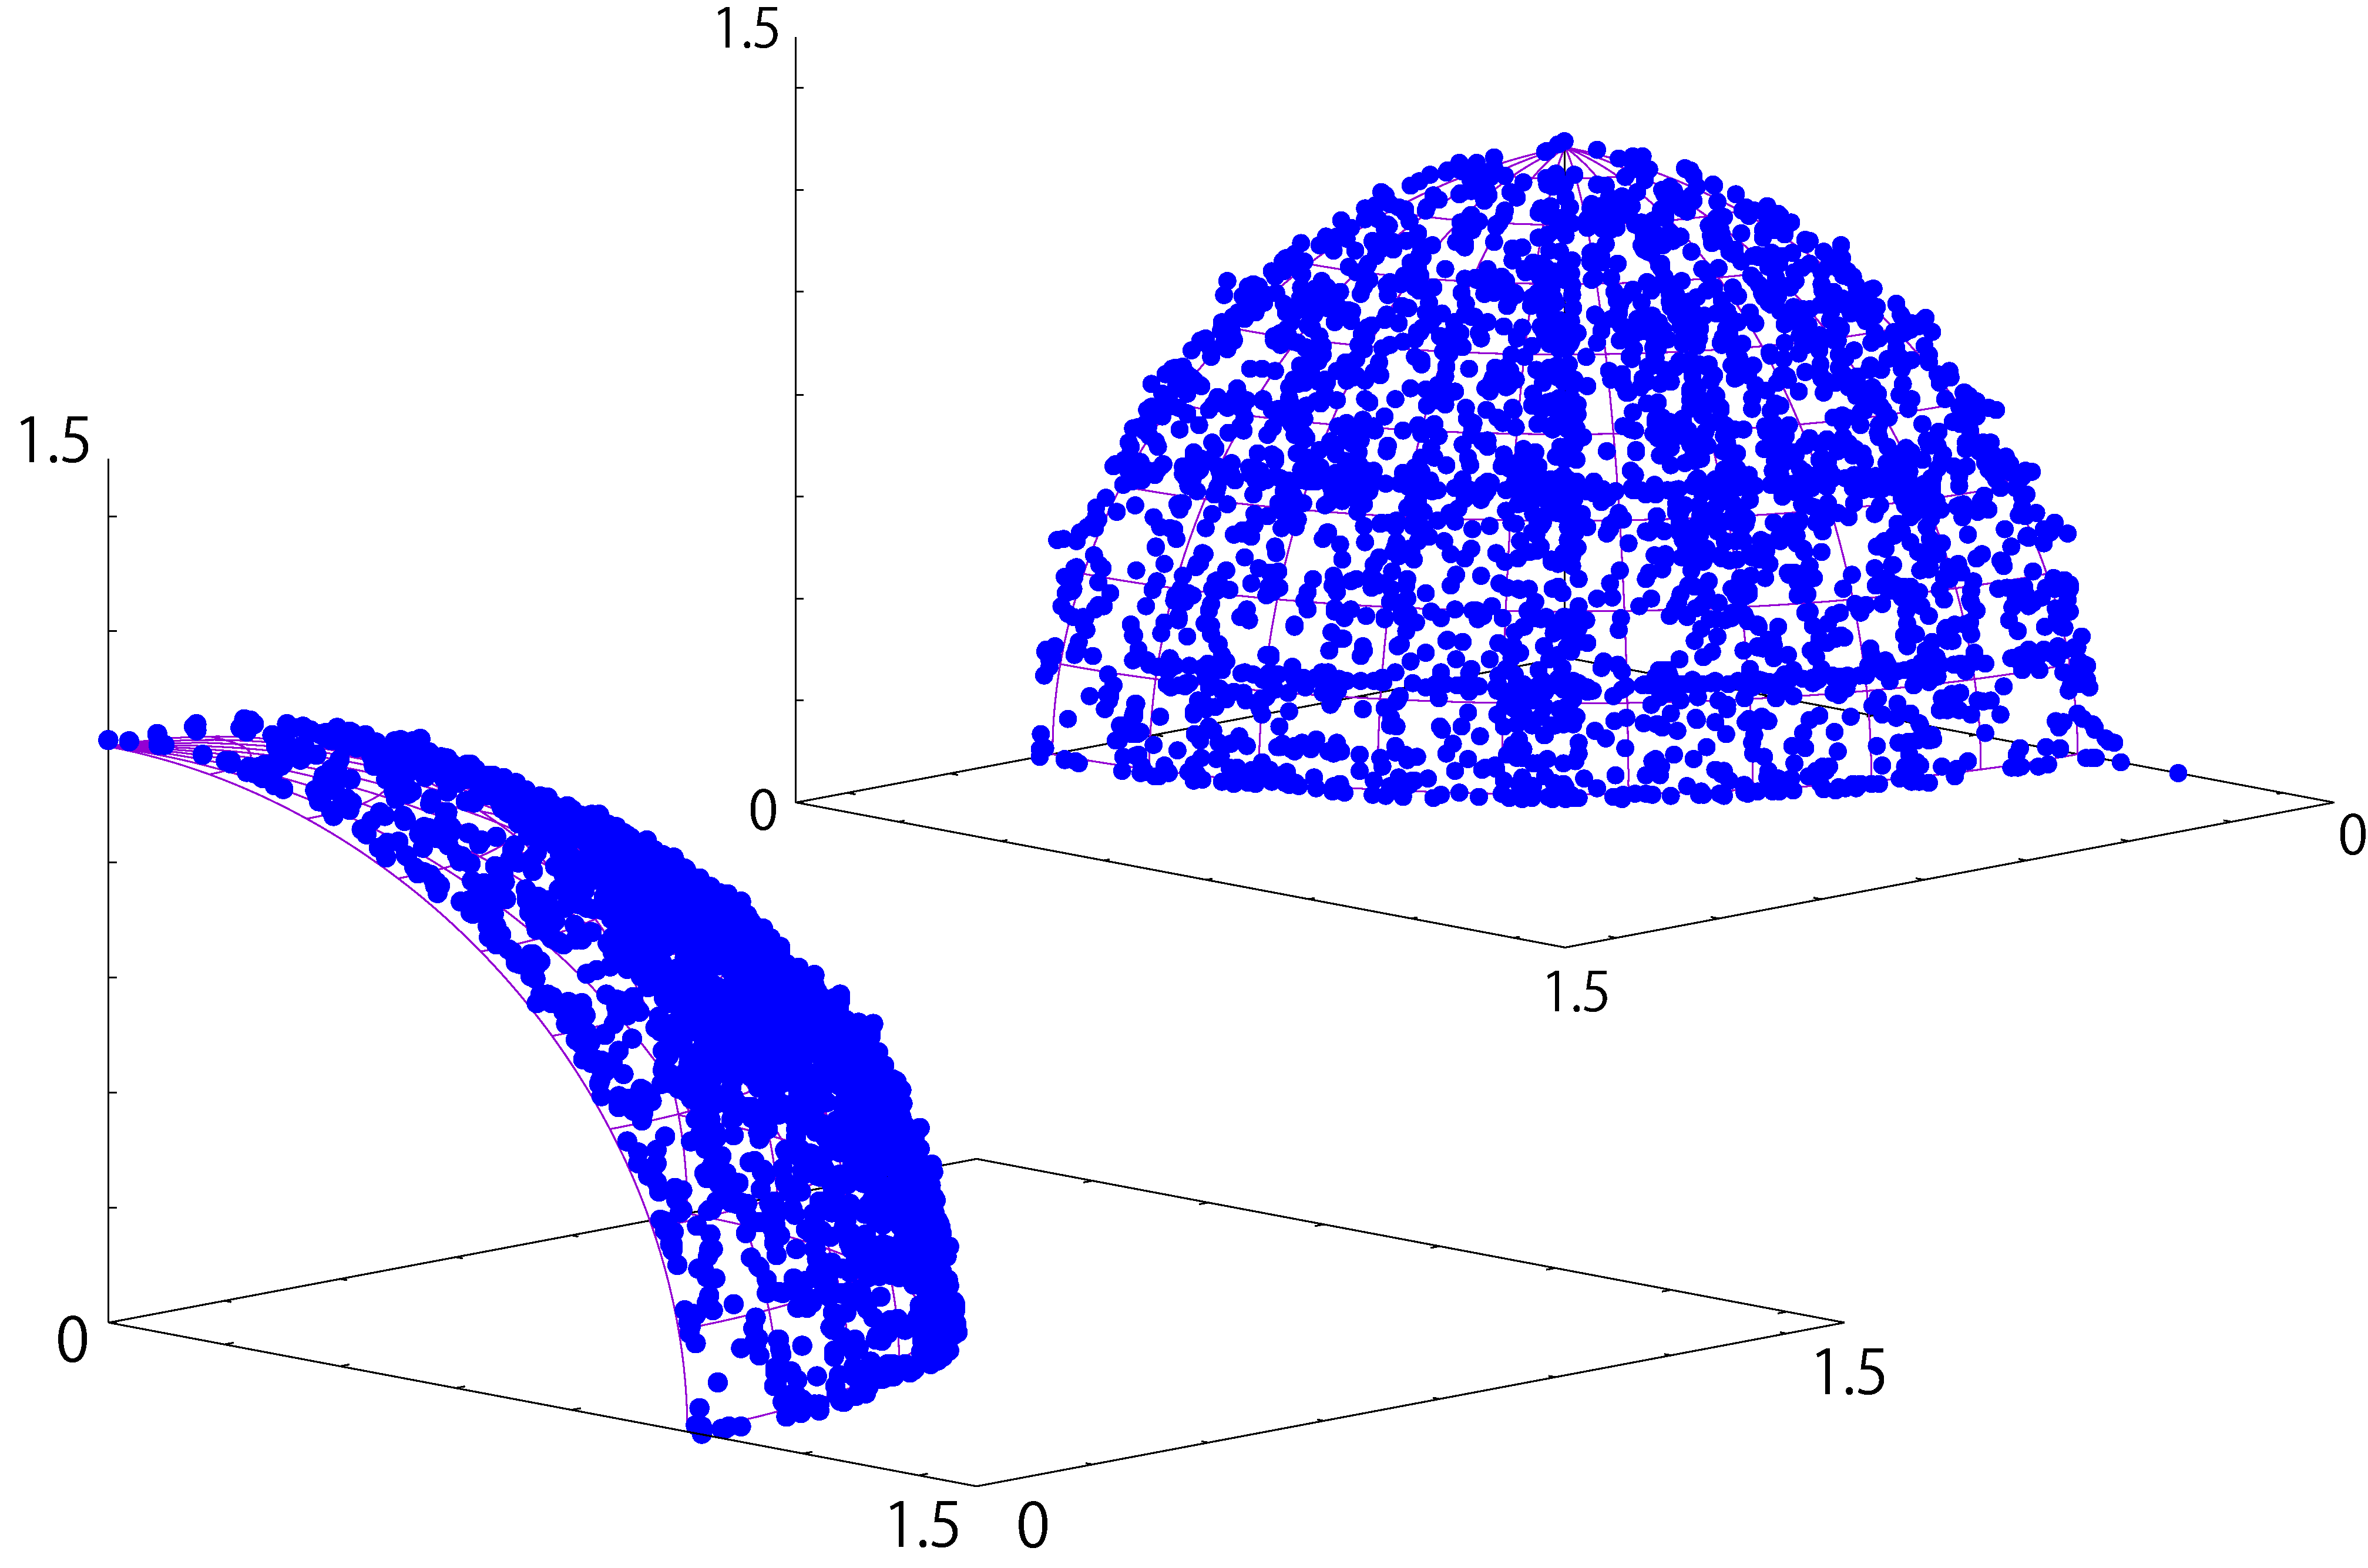
\includegraphics[width=1\linewidth]{../figures/multidtlz4_kde_double.pdf}
\begin{center}
{\footnotesize (b) ePDF}
\end{center}
\end{minipage}
\begin{minipage}{0.33\hsize}
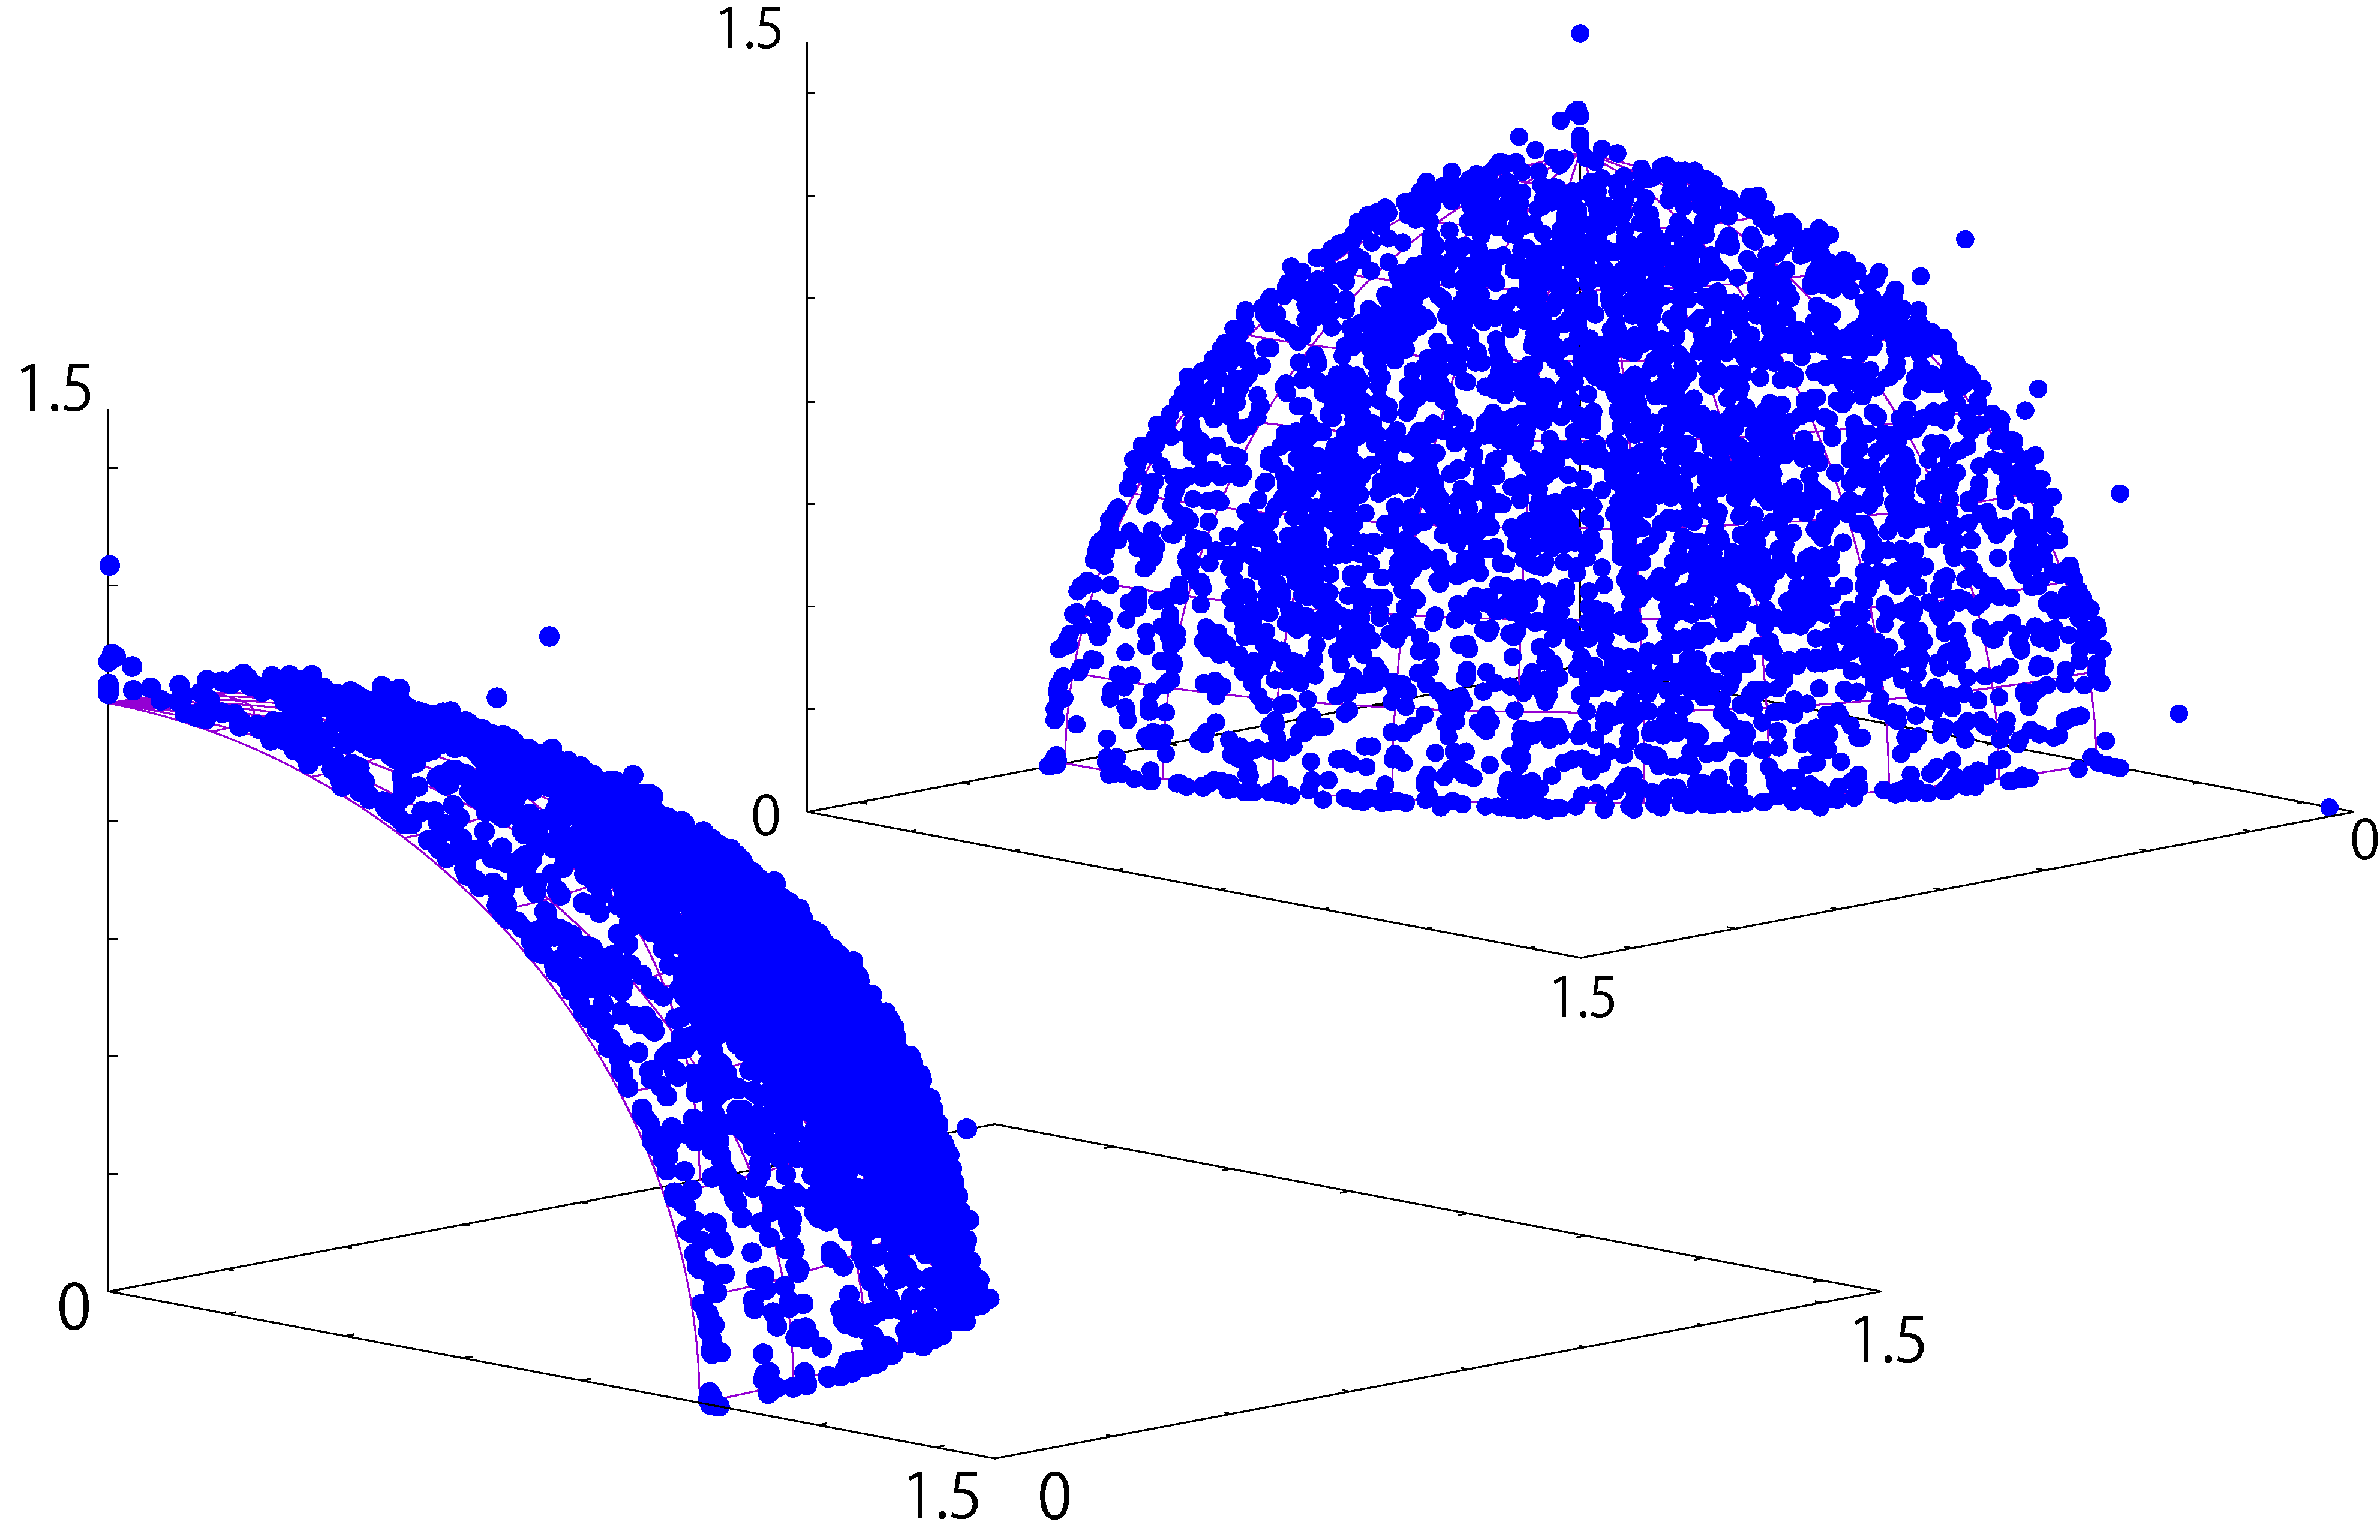
\includegraphics[width=1\linewidth]{../figures/multidtlz4_uc_double.pdf}
\begin{center}
{\footnotesize (c) 制御なし}
\end{center}
\end{minipage}
\end{tabular}
\caption{適応的離散化手法を用いた場合と用いない場合のModified DTLZ4における非劣解の分布}
\label{fig:nondoms_multidtlz4}
\end{figure*}

\begin{figure*}[!h]
\begin{minipage}{0.38\hsize}
\vspace{-0.2in}
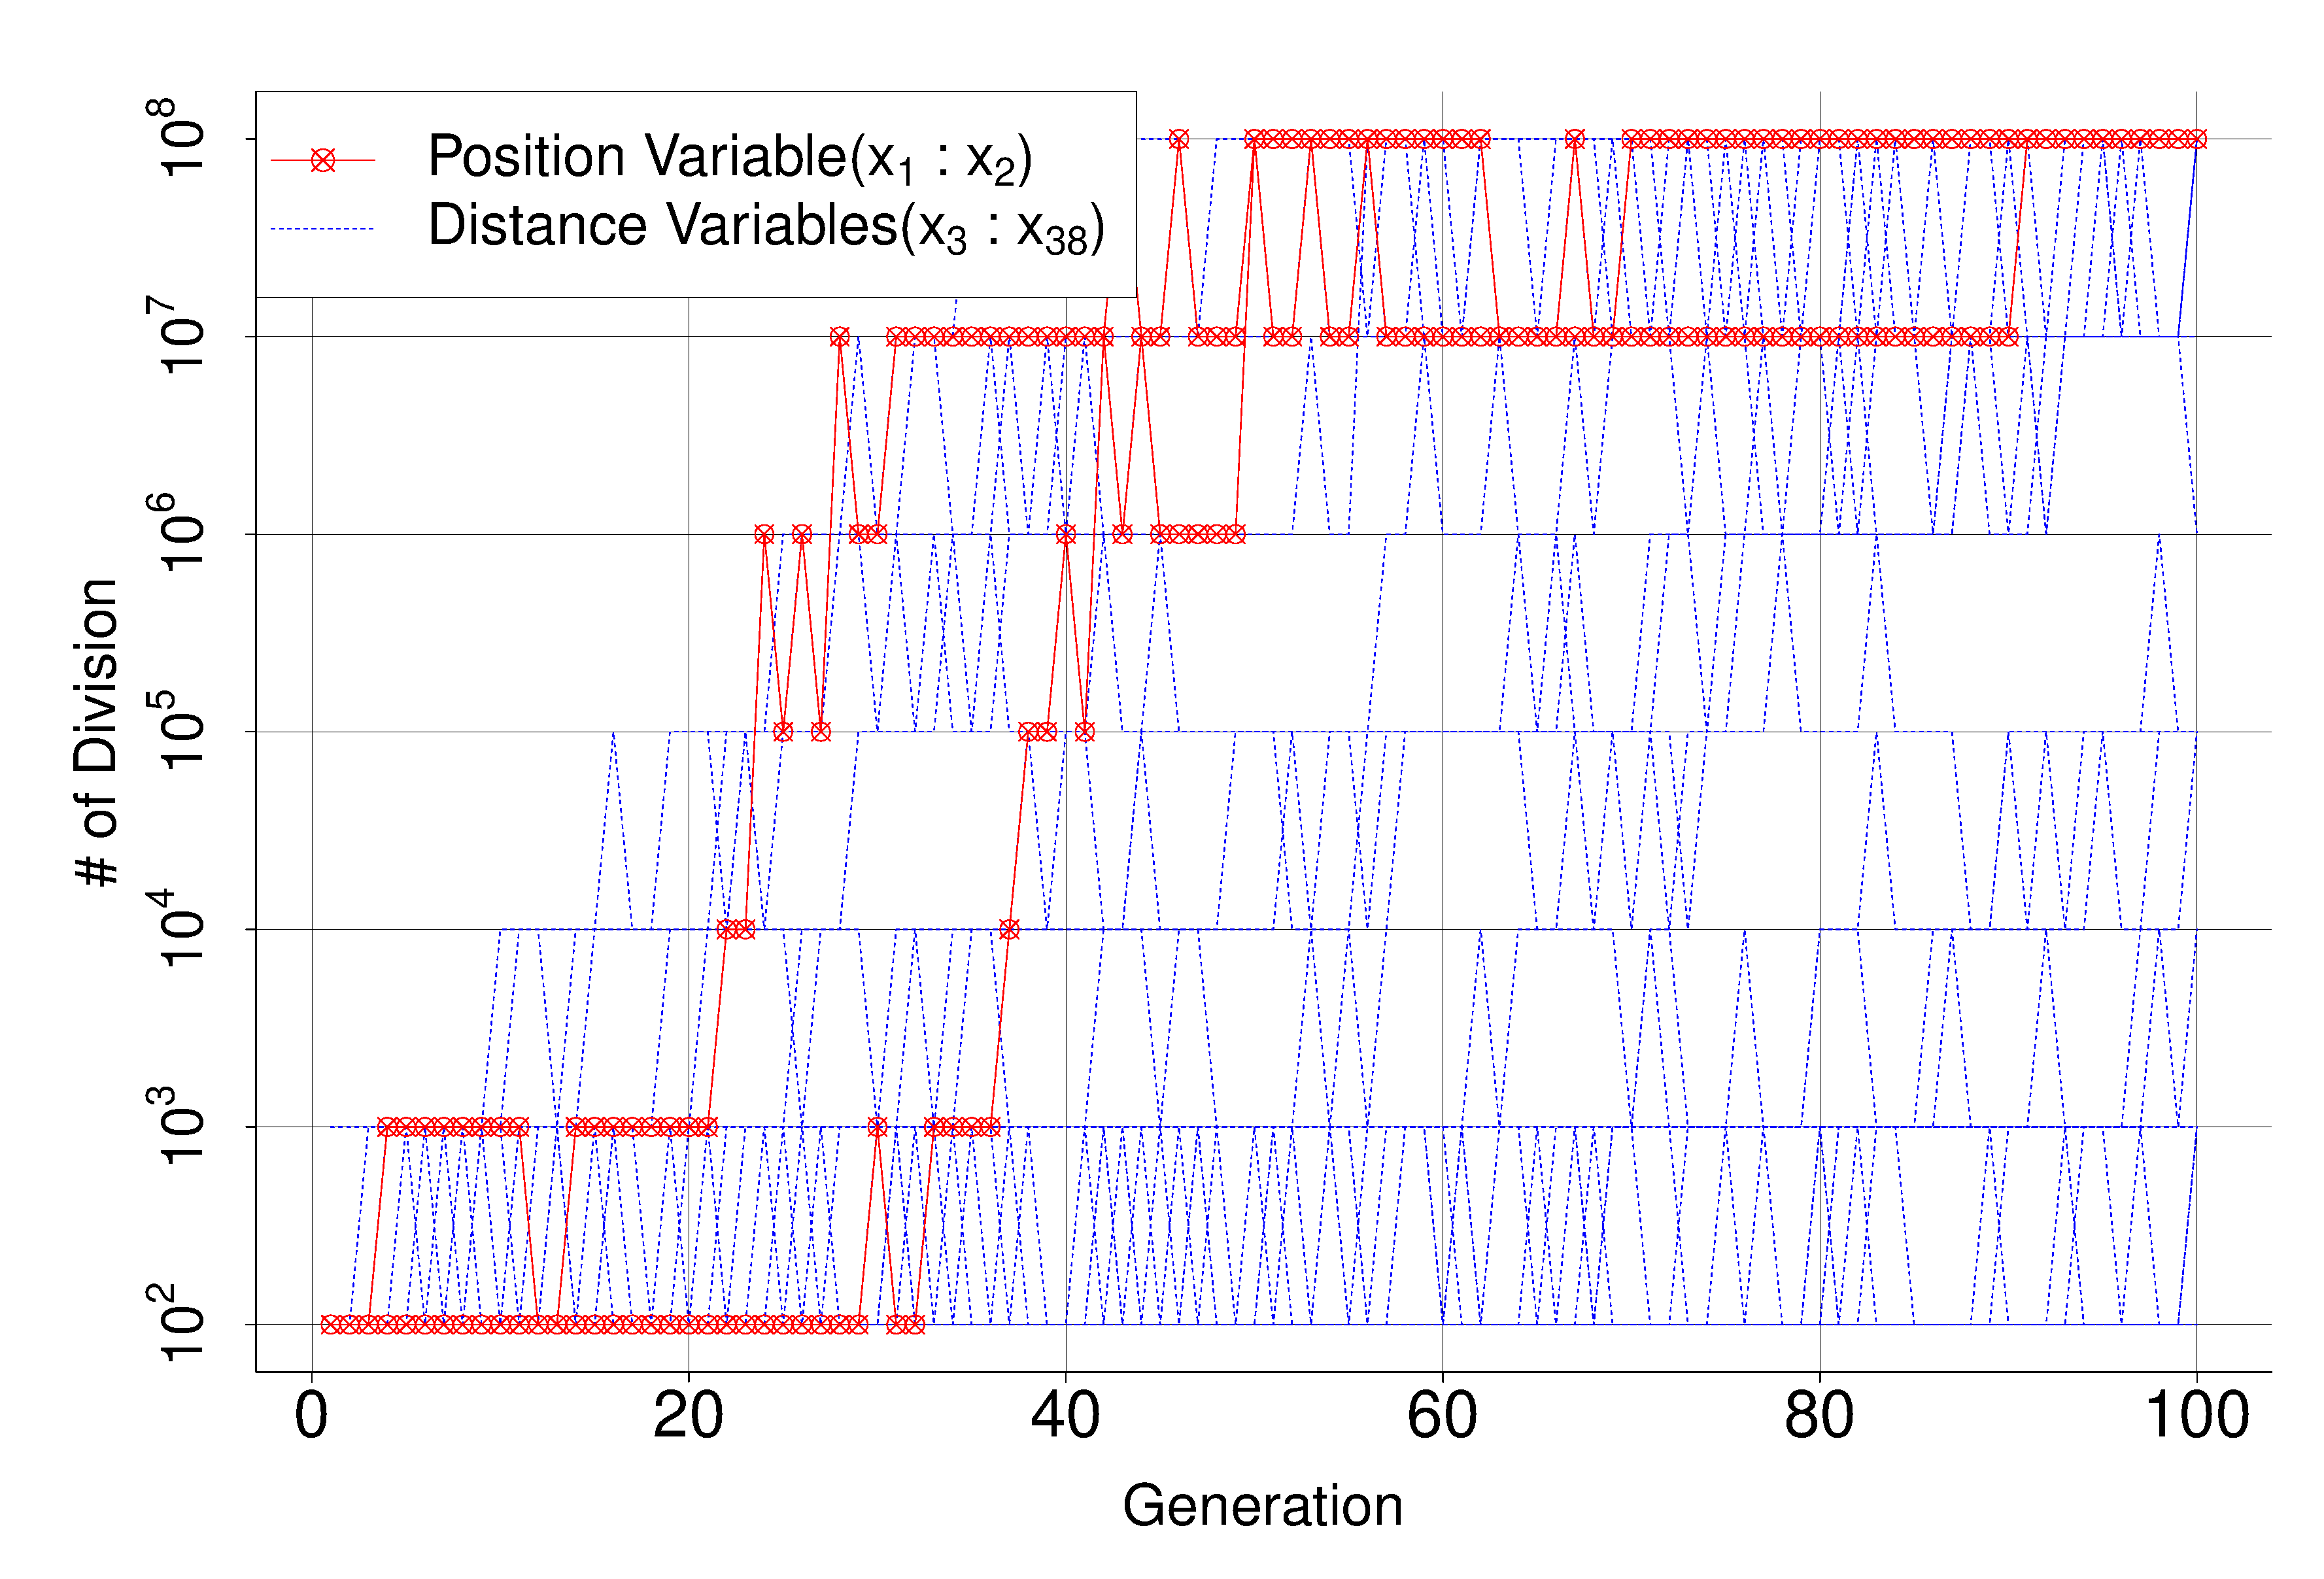
\includegraphics[width=1\linewidth]{../figures/multi_DTLZ4_digit_trend.eps}\\
\\
\caption{The transition of division number in WFG7.}
\label{digi_trans_multidtlz4}
\end{minipage}
\begin{minipage}{0.61\hsize}
\begin{minipage}{0.49\hsize}
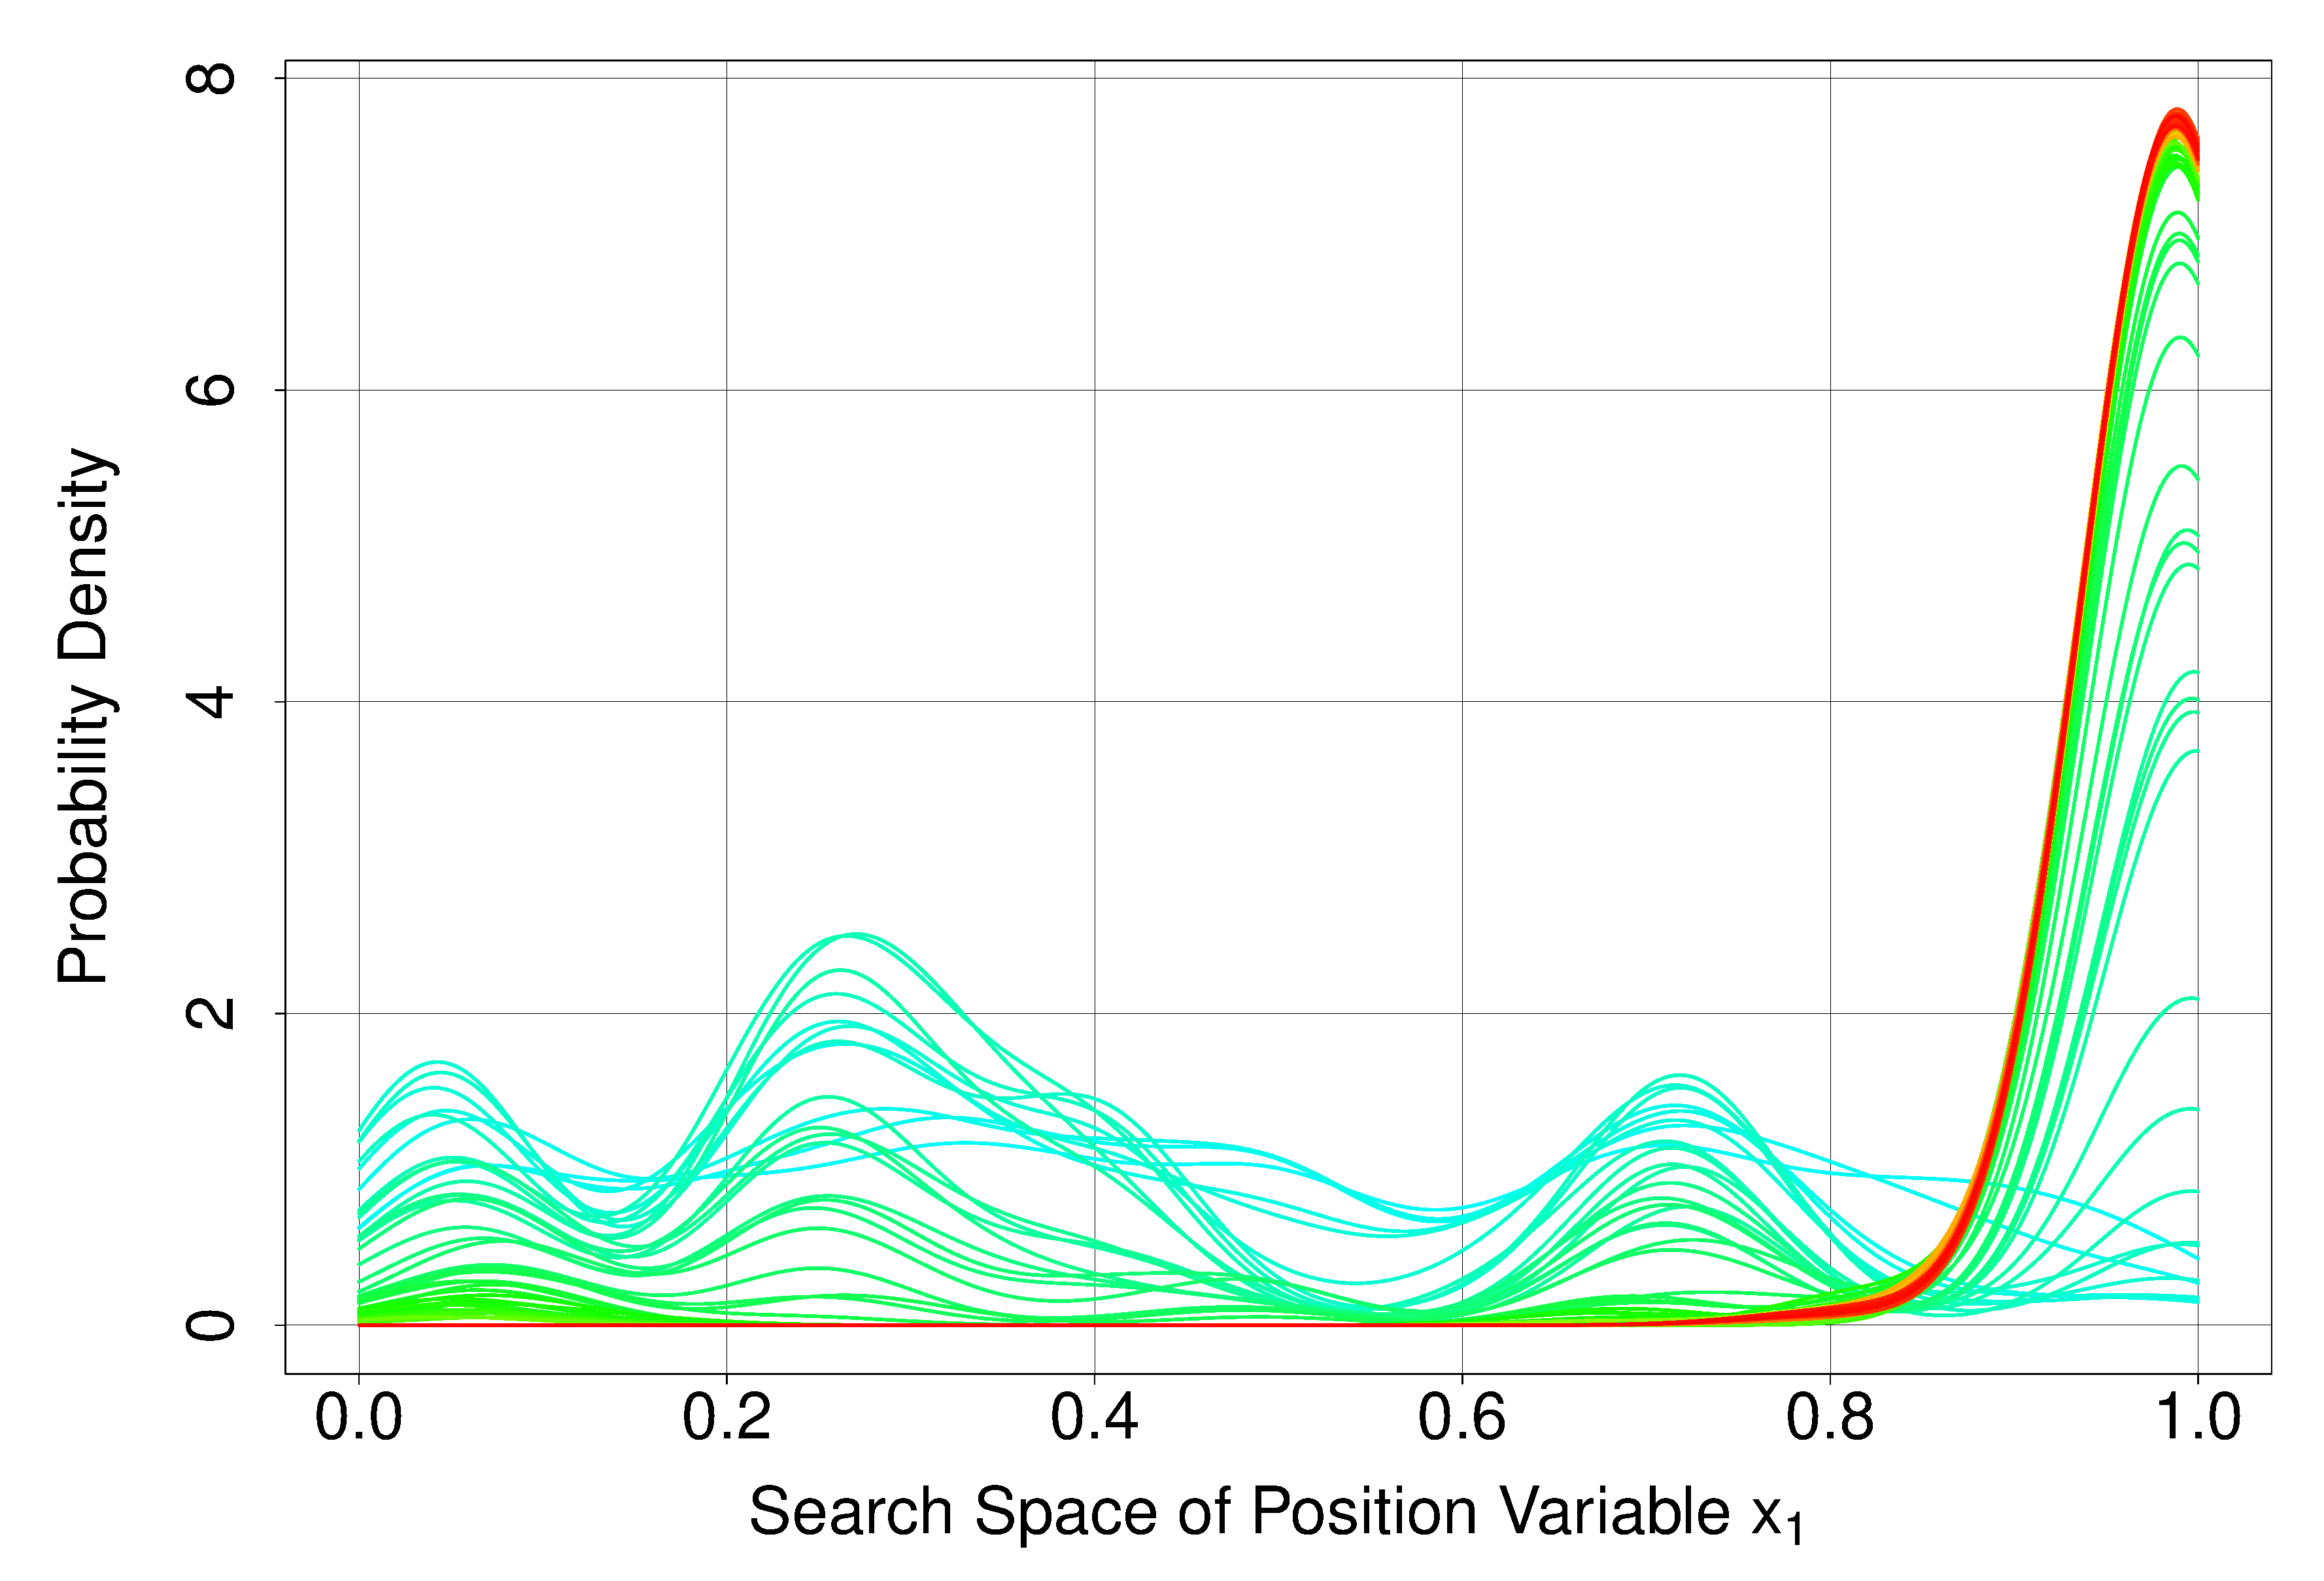
\includegraphics[width=1\linewidth]{../figures/multi_DTLZ4_var1_pdf_trend.eps}\\
\centering
\hspace{0.2in} \includegraphics[width=0.8\linewidth]{../figures/color_bar_100ver.eps}
\begin{center}
{\footnotesize (a) 位置変数$x_1$における推定された確率密度関数の推移}
\end{center}
\end{minipage}
\begin{minipage}{0.49\hsize}
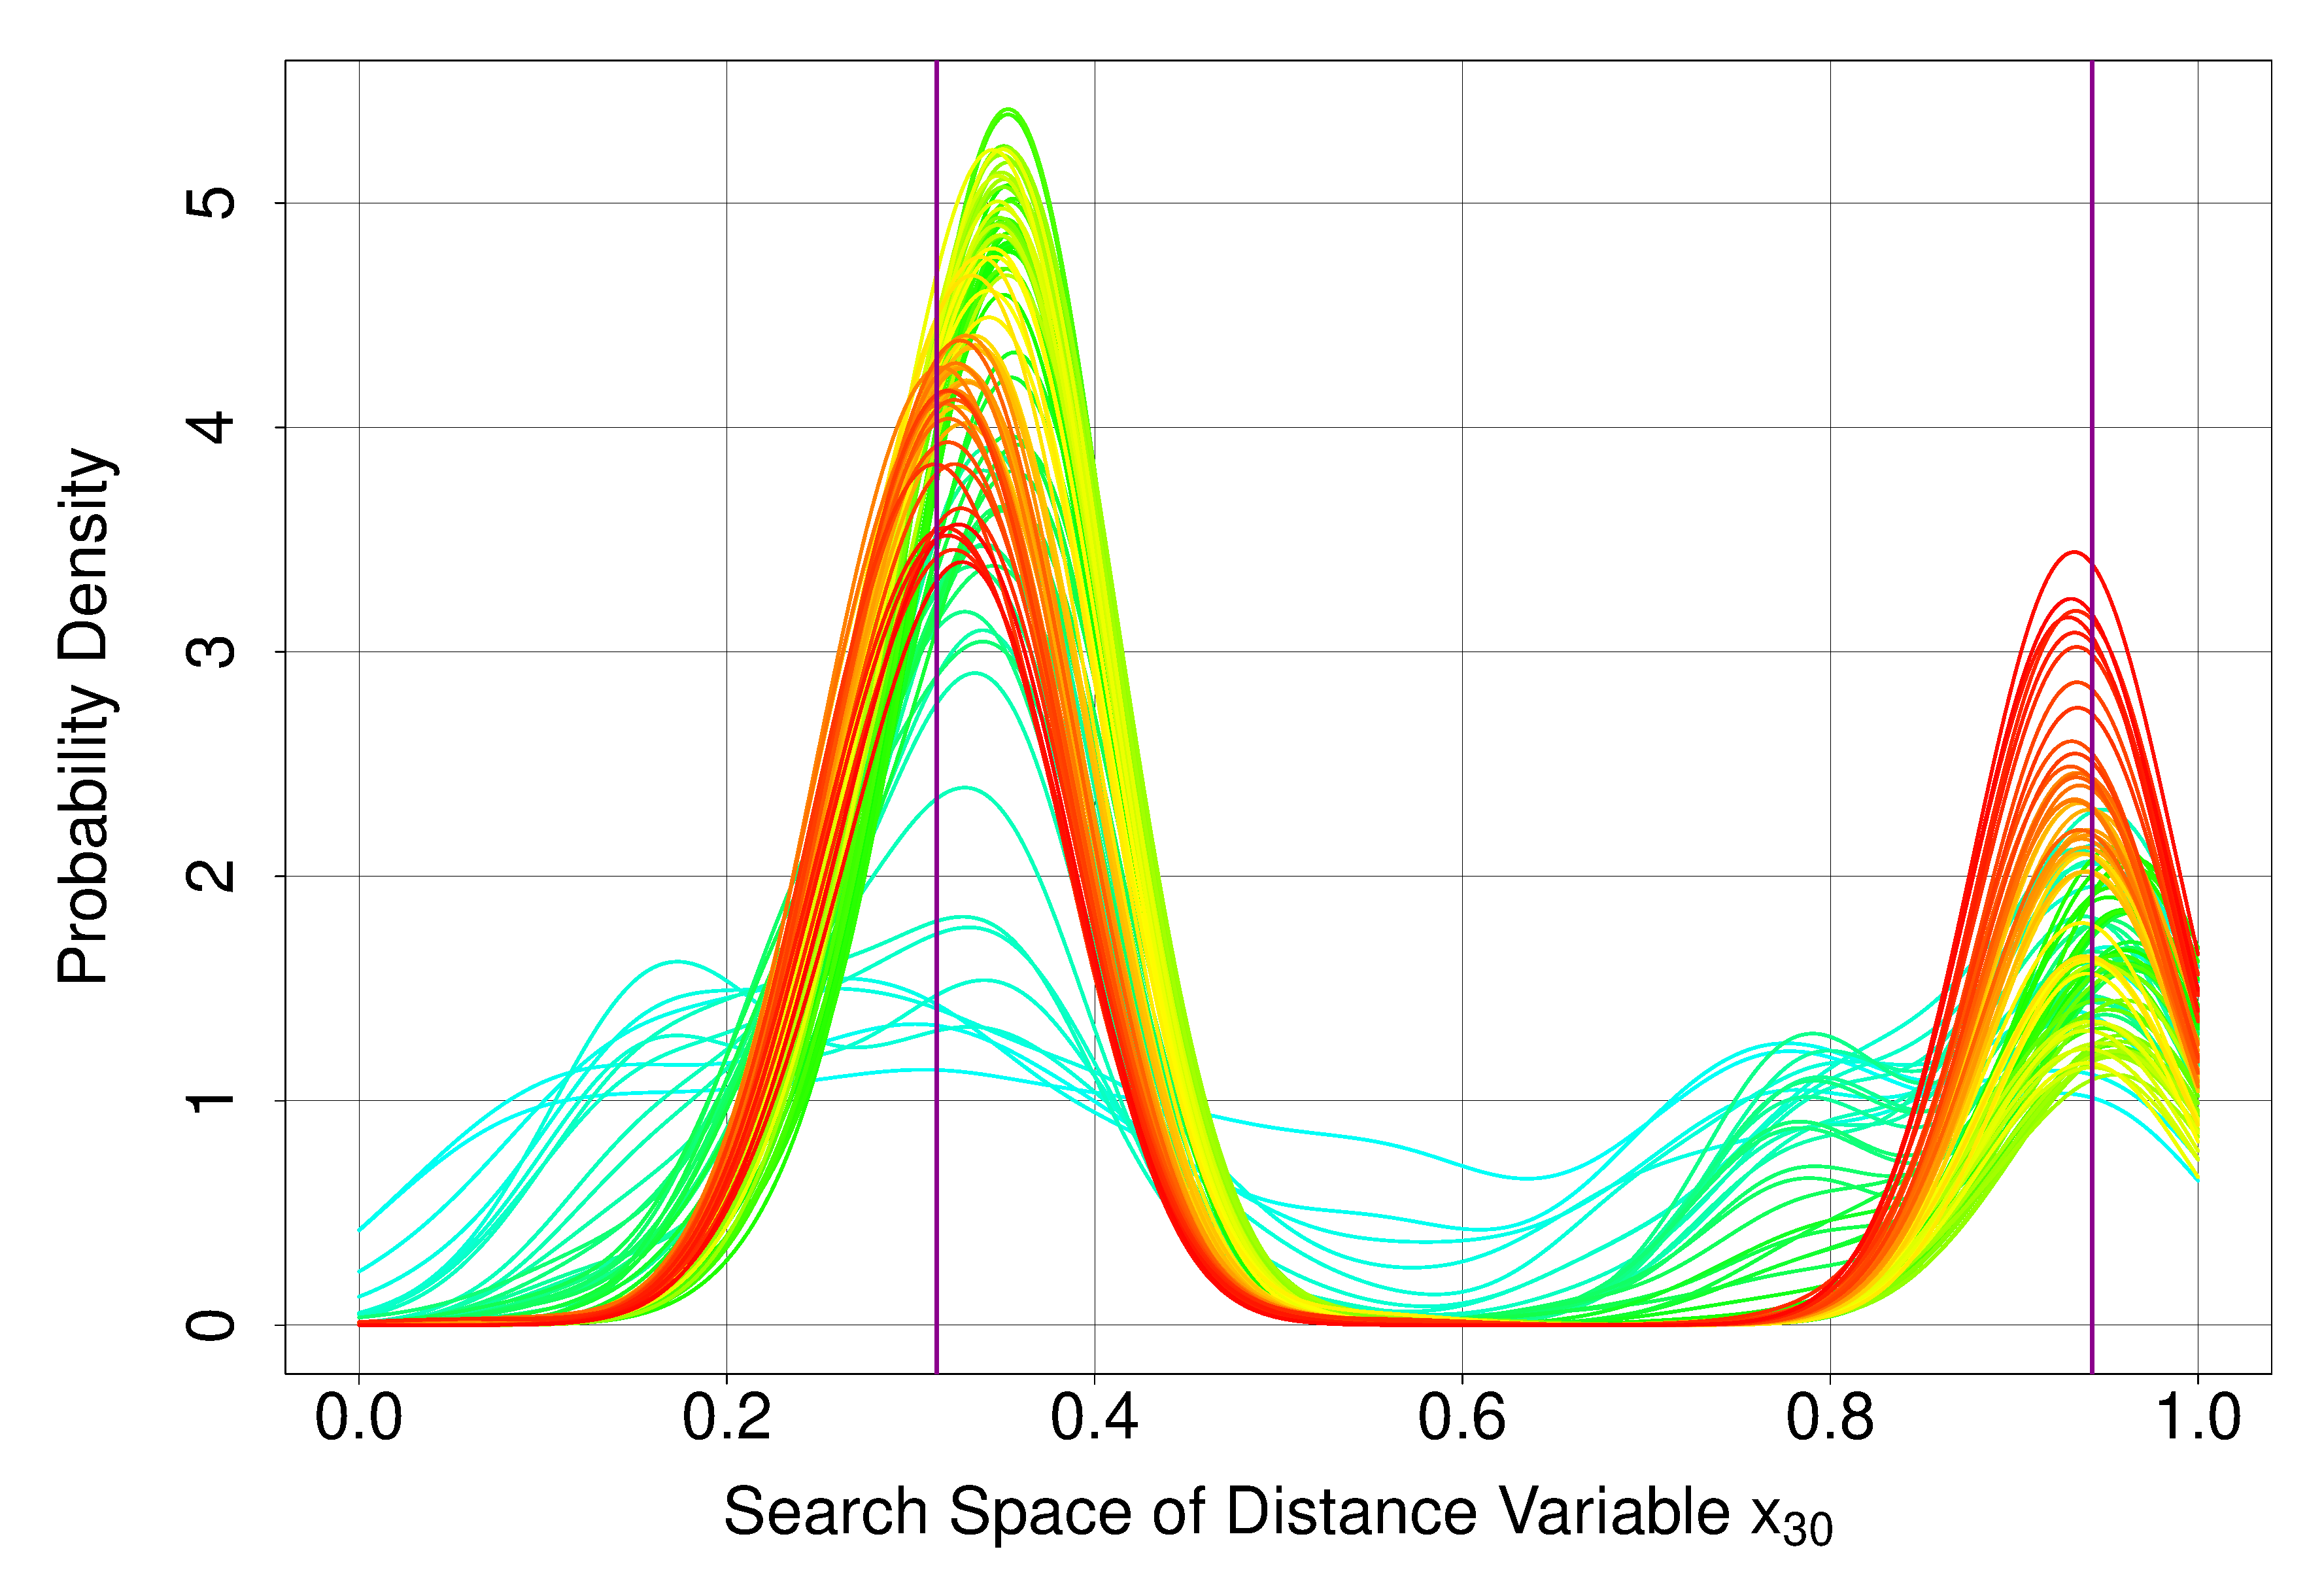
\includegraphics[width=1\linewidth]{../figures/multi_DTLZ4_var30_pdf_trend.eps}\\
\centering
\hspace{0.2in} \includegraphics[width=0.8\linewidth]{../figures/color_bar_100ver.eps}
\begin{center}
{\footnotesize (b) 距離変数$x_{10}$における推定された確率密度関数の推移}
\end{center}
\end{minipage}
\caption{ePDFを用いた場合のMulti DTLZ4における推定された確率密度関数の世代ごとの推移}
\label{pdf_trans_multidtlz4}
\end{minipage}
\label{fig:nondom_sol}
\end{figure*}

\clearpage

\Figref{pdf_trans_multidtlz4}は,ePDFを用いた場合に各世代におけるある設計変数空間の分布について推定された確率密度関数を示しており,(a)は位置変数である$x_1$,(b)は距離変数である$x_{30}$について得られた確率密度関数を示している.
縦軸は確率密度,横軸は設計変数空間を正規化空間に射影した際の探索空間を示しており[0,1]の範囲であり,確率密度関数の色は推定された世代を示している.
また,\Figref{pdf_trans}(b)における図中の紫の縦線は真の最適値を示している.
ePDFを用いた適応的離散化では,確率密度が高いほど細かく離散化が行われる.
\Figref{pdf_trans_multidtlz4}(a)より,位置変数$x_1$では世代を経るごとに1付近の確率密度が高い値となっていることから,1付近の解は細かく離散化されていることが分かる.
Multi DTLZ4は,先行研究の結果から0.9-1の間を細かい粒度で探索しなければ多様な解が得られないことが分かっている.
このことから,ePDFを用いた適応的離散化は細かい粒度を必要とする領域において適切に細かい探索に切り替えることができることが分かった.
また,このように離散化できたことにより,優れたIGDになったと考えられる.
\Figref{pdf_trans_multidtlz4}(b)より,距離変数$x_{30}$では世代を経るごとに0.3,0.9付近の確率密度が高い値となっていることから,これらの付近の解は細かく離散化されていることが分かる.
Multi DTLZ4は距離変数に最適値を二つ持つ問題であり,\Figref{pdf_trans_multidtlz4}(b)に紫の線で示した箇所に最適値が存在する.
ePDFではこれら二つの最適値周辺を細かく離散化することができており,設計の意図通りに機能していることが分かる.
しかし,Multi DTLZ4では,最適値のどちらか一方が得られれば収束するため,二つの解を同時に探索する必要はない.
そのため,このことが収束性向上にあまり影響していないことが分かる.
しかしながら,設計変数同士に相関関係があり,同一設計変数空間上において二つの解を同時に探索する必要のある問題では,効果的に探索を進めることができると考えられる.

さらに,\Figref{multidtlz4_igd_transition}の結果から,ePDFとその他で大きな差が見られるものの,\Figref{fig:nondoms_multidtlz4}では解の多様性に大きな差が見られない原因を探るため,各提案手法と離散制御なしで得られたIGD値の最大値と最小値の推移を比較する.
\Figref{fig:minmax}は,各提案手法と離散制御なしで得られたIGD値の最大値と最小値の世代ごとの推移を示しており,実線で示される推移は平均値の推移,塗りつぶされた領域は最大値と最小値に囲まれた領域を表す.
\Figref{fig:minmax}の結果から,SDと離散制御なしは最大値と最小値の差が大きいことが分かる.
このことから,SDと離散制御なしは初期集団の違い等,試行ごとに結果に偏りが生じやすいことが分かる.
一方で,ePDFの結果を見ると最大値と最小値の差が非常に小さいことが分かる.
ePDFは最大値と最小値の差が非常に小さいため,優れたIGD値の平均値となっていたことが分かった.
他のベンチマーク問題についても,ePDFは最大値と最小値の差が非常に小さい結果が得られている.
このことから,ePDFは試行ごとのばらつきを小さくする性能があることが示唆される.


\begin{figure*}[htbp]
\begin{tabular}{cc}
\begin{minipage}{0.33\hsize}
\includegraphics[width=1\linewidth]{../figures/multidtlz4_sd_minmax.png}
\begin{center}
{\footnotesize (a) SD}
\end{center}
\end{minipage}
\begin{minipage}{0.33\hsize}
\includegraphics[width=1\linewidth]{../figures/multidtlz4_epdf_minmax.png}
\begin{center}
{\footnotesize (b) ePDF}
\end{center}
\end{minipage}
\begin{minipage}{0.33\hsize}
\includegraphics[width=1\linewidth]{../figures/multidtlz4_uc_minmax.png}
\begin{center}
{\footnotesize (c) 制御なし}
\end{center}
\end{minipage}
\end{tabular}
\caption{適応的離散化手法を用いた場合と用いない場合のMulti DTLZ4におけるIGDの最大値と最小値の推移}
\label{fig:minmax}
\end{figure*}

\section{適応的離散化手法の性能評価のまとめ}
\quad 数値実験の結果から,適応的離散化手法を用いることで多くの問題において離散化を行わない場合と同等かそれ以上の収束性能を示すことがわかった.
また,適応的離散化を用いることでIGDが悪化してしまう問題も見られたが,同程度のオーダーのIGD値を得ることができた.
また,実際の非劣解の分布を確認すると離散化の制御をしないものに比べ多様性に大きな違いも見られなかった.
これらの結果から,適応的離散化を用いることで多様性をある程度維持しながらも収束性を向上させることができると考えられる.
さらに,SDを用いた離散化手法では,設計変数ごとに細かい粒度が必要な設計変数とそうでない設計変数を識別することができており,実際の設計問題においても有用な知見が得られる可能性があると考えられる.
ePDFを用いた離散化手法では,設計変数同士に相関を持つような問題や最適値を同時に複数個探索しなければならないような問題に対して,期待したメカニズムが有効に機能することが示唆された.
また,試行ごとのばらつきを抑える性能があることが示唆された.


\end{document}